\documentclass[conference]{IEEEtran}

\usepackage{graphicx}
\graphicspath{{output_image/}{./output_image/}{./}{../output_image/}}
\usepackage{amsmath}
\usepackage{amssymb}
\usepackage{url}
\usepackage{cite}
\usepackage{booktabs}
\usepackage{array}
\usepackage{xcolor}
\usepackage[bookmarks=false]{hyperref}
\extrafloats{100}
\providecommand{\appendices}{\appendix}

% High float allowances to prevent blank spaces and premature float pages
\renewcommand{\topfraction}{0.95}
\renewcommand{\bottomfraction}{0.95}
\renewcommand{\textfraction}{0.05}
\renewcommand{\floatpagefraction}{0.60}
\renewcommand{\dbltopfraction}{0.95}
\renewcommand{\dblfloatpagefraction}{0.55}
\setcounter{topnumber}{4}
\setcounter{bottomnumber}{4}
\setcounter{totalnumber}{10}
\setcounter{dbltopnumber}{4}

% Eliminate top and bottom float whitespace gaps
\makeatletter
\setlength{\@fptop}{0pt}
\setlength{\@fpbot}{0pt plus 1fil}
\setlength{\@fpsep}{4pt plus 1pt minus 1pt}
\setlength{\@dblfptop}{0pt}
\setlength{\@dblfpbot}{0pt plus 1fil}
\setlength{\@dblfpsep}{4pt plus 1pt minus 1pt}
\makeatother

% Prevent vertical paragraph stretching between columns
\raggedbottom
\setlength{\parskip}{0pt plus 0.5pt}

% Tight, consistent spacing between floats, captions, and body text
\setlength{\textfloatsep}{6pt plus 2pt minus 2pt}
\setlength{\floatsep}{6pt plus 2pt minus 2pt}
\setlength{\dbltextfloatsep}{6pt plus 2pt minus 2pt}
\setlength{\dblfloatsep}{6pt plus 2pt minus 2pt}
\setlength{\intextsep}{6pt plus 2pt minus 2pt}
\setlength{\abovecaptionskip}{3pt plus 1pt minus 1pt}
\setlength{\belowcaptionskip}{2pt plus 1pt minus 1pt}

\hypersetup{colorlinks=true, linkcolor=blue, citecolor=blue, urlcolor=blue}

\title{A Machine Learning Framework for Daily Rainfall Classification and Extreme Event Analysis in the Kathmandu Watershed, Nepal}

\author{
\IEEEauthorblockN{Sadhana Adhikari}
\IEEEauthorblockA{
MSc Data Science and Computational Intelligence\\
Softwarica College of IT and E-Commerce, Coventry University\\
Kathmandu, Nepal\\
Student ID: 260102 \quad CUID: 17625409\\
Email: 260102@softwarica.edu.np
}
}

\begin{document}
\setkeys{Gin}{draft=false}

\maketitle
\sloppy\hbadness=10000\vbadness=10000

\begin{abstract}
Heavy rainfall and extreme storm events cause frequent floods and landslides in mountain valleys. This study presents a practical machine learning workflow to analyze daily rainfall patterns and classify rainfall intensity across the Kathmandu watershed. We combined 10 years of daily ground measurements (2016--2025; $69{,}407$ station-days) from 19 Department of Hydrology and Meteorology (DHM) stations with Global Precipitation Measurement (GPM) IMERG V07 satellite data. Direct comparison showed that raw satellite data tends to overestimate light rain (mean bias of $+2.78\text{ mm/day}$) and produces frequent false alarms ($\text{FAR} = 46.12\%$). Using unsupervised Principal Component Analysis (PCA) and K-Means clustering, we identified three distinct rainfall zones shaped by elevation. To address severe class imbalance ($86.11\%$ light rain vs. only $0.11\%$ very heavy and extreme rain), we trained regularized Random Forest, XGBoost, and feature-scaled Support Vector Machines (Linear and RBF kernels) using a strict chronological split (2016--2022 training, 2023--2024 validation, and 2025 independent test) along with Leave-One-District-Out spatial testing. On the 2025 test set ($N = 6{,}935$), feature-scaled Linear SVM achieved the highest overall accuracy ($74.72\%$, weighted F1: $78.92\%$, macro F1: $0.3682$). Random Forest achieved the highest balanced accuracy ($59.80\%$, macro F1: $0.3446$), successfully detecting $80.00\%$ of very heavy storms. XGBoost achieved $70.48\%$ accuracy, delivered the best recall on heavy storms ($42.65\%$), and reached the highest Macro ROC-AUC ($0.88$). Spatial testing confirmed reliable performance across all three districts ($71.21\%$--$75.85\%$ accuracy). SHAP analysis revealed that rainfall from the previous 1 to 3 days had the strongest influence on model predictions ($74.47\%$ relative gain for 1-day lag; $9.47\%$ for 3-day lag). Finally, Mann--Kendall trend tests confirmed a statistically significant rise in annual average rainfall ($\tau = +0.5111$, $p = 0.0491$, $Q = +0.2012\text{ mm/year}$), while daily maximums ($+2.4800\text{ mm/year}$) and extreme events ($+0.8889\text{ events/year}$) showed positive upward trends, providing useful benchmarks for local flood warning and disaster planning.
\end{abstract}

\begin{IEEEkeywords}
Rainfall variability, extreme rainfall, machine learning, GPM IMERG V07, Kathmandu Valley, Bagmati Basin, Random Forest, XGBoost, Support Vector Machines, SHAP, Mann--Kendall.
\end{IEEEkeywords}

\section{Introduction}
\label{sec:introduction}

Precipitation is one of the most critical meteorological variables driving the hydrological cycle, directly impacting agricultural productivity, water resource management, and the frequency of natural disasters such as floods and landslides. In topographically complex regions like the Himalayas, characterized by extreme elevation gradients and heterogeneous microclimates, accurate measurement and classification of rainfall intensity are paramount. The Kathmandu watershed, situated within this fragile mountainous ecosystem, exemplifies the urgent need for precise precipitation monitoring. The region heavily relies on the South Asian summer monsoon, which delivers over 80\% of its annual rainfall in a concentrated three-to-four-month window. Consequently, deviations in precipitation patterns not only threaten water security but also escalate the vulnerability of dense urban populations to severe hydrometeorological hazards. Accurately classifying and predicting rainfall intensity across this variable terrain is therefore a critical priority for policymakers, hydrologists, and disaster risk reduction agencies.

\subsection{Rainfall Patterns, Climate Trends, and Urban Hazards}
Rainfall variability and extreme storm events are closely connected to climate change, especially in high-relief mountainous regions like the Hindu Kush Himalaya. As global temperatures rise, warmer air holds more water vapor---increasing by about $7\%$ for every $1^\circ\text{C}$ of warming, as described by the Clausius--Clapeyron relation. In mountainous terrain, this warming effect is often stronger at higher altitudes. This process alters atmospheric moisture transport and changes how the South Asian summer monsoon delivers rain across the region. Consequently, climate change often appears not just as a change in annual totals, but as increased rainfall variability: longer dry periods broken by sudden, short, and intense rainfall events. In a bowl-shaped and rapidly urbanizing valley like Kathmandu, this changing pattern drastically increases environmental hazards. Heavy downpours can quickly exceed the capacity of soil and drainage channels, leading to flash floods along the Bagmati River and its tributaries---including Bishnumati, Dhobi Khola, Hanumante, and Nakkhu Khola---as well as landslides on steep surrounding ridges. Analyzing rainfall variability and accurately classifying extreme events is therefore vital for municipal disaster planning, urban drainage modernization, and practical flood early warning systems.

Historically, meteorological monitoring in high-relief terrain has depended on sparse networks of physical rain gauges. While ground stations provide ground truth observations, their spatial density is inadequate to capture microclimatic variability. Satellite precipitation products offer continuous spatial coverage, yet extensive evaluations in complex topography confirm that raw satellite retrievals suffer from significant spatial and elevational biases \cite{sharma2020}. Concurrently, climatological trend investigations demonstrate that the temporal distribution of extreme convective downpours is intensifying across regional basins \cite{khanal2024}. To overcome these non-linear discrepancies, contemporary machine learning architectures have emerged to map satellite estimates and topographic context to localized rainfall intensity \cite{lei2025}. Supporting investigations have quantified elevational dependencies in satellite retrieval errors \cite{Tang2020}, while global satellite retrieval algorithms document the technical calibration procedures of the IMERG V07 product \cite{Huffman2020}.

Despite the proliferation of satellite data and the growing body of literature evaluating its accuracy, a significant research gap remains in the operational integration of these datasets for localized, high-resolution predictive modeling in complex terrains. Traditional statistical downscaling and interpolation techniques often fail to capture the non-linear, multidimensional relationships between satellite estimates, topographical features (such as elevation and geographic coordinates), and ground-based observations. While machine learning (ML) has seen rapid adoption in hydrology for tasks such as streamflow forecasting and anomaly detection, its application to the systematic classification of localized rainfall intensity using blended satellite and topographic data remains underexplored in complex high-relief terrain analysis. Furthermore, many existing ML applications in this domain prioritize absolute predictive accuracy over model interpretability and generalization, frequently resulting in highly complex, overfitted models that perform poorly when deployed in resource-constrained operational environments or when confronted with unprecedented extreme weather events.

\subsection{Problem Statement}
Rainfall in the Kathmandu watershed exhibits substantial spatial and temporal variability due to complex topography, surrounding mountain ridges, and seasonal monsoon processes. The occurrence of heavy and extreme rainfall creates severe risks for urban drainage, rapid riverine flash floods, hill-slope landslides, and water-resource infrastructure. This investigation addressed three primary problem dimensions:

First, the basin's dramatic vertical elevation gradients (spanning approximately 1,200 masl at the Chobhar drainage outlet to over 2,700 masl on surrounding mountain crests across the 587 km$^2$ watershed) induce pronounced orographic microclimates. Over 80\% of annual rainfall is concentrated within a narrow four-month summer monsoon window, causing sharp localized precipitation contrasts that standard spatial interpolation tools fail to capture.

Second, an acute observational dilemma exists between terrestrial rain gauges and satellite products. Ground gauges from the Department of Hydrology and Meteorology (DHM) provide accurate measurements but suffer from spatial sparsity (19 operational stations across three districts). Gridded satellite products such as GPM IMERG V07 offer regional coverage but contain pronounced high-altitude retrieval uncertainties, elevated false alarms (FAR = 46.12\%), and systemic positive mean biases (+2.78 mm/day) over Himalayan terrain.

Third, daily precipitation datasets exhibit profound class imbalance: across the 69,407 station-day records (2016--2025), light rainfall ($< 10$ mm/day) spans 86.11\% (59,768 days), whereas combined very heavy ($100$--$200$ mm/day; 66 days, 0.10\%) and extreme ($\ge 200$ mm/day; 9 days, 0.013\%) events constitute only 0.11\% ($< 0.5\%$) of observations. Conventional machine learning models trained on unscaled or unweighted data risk algorithmic collapse, preferentially predicting majority light-rainfall conditions while failing to detect rare extreme hazards. Furthermore, a short 10-year (2016--2025) observational record cannot establish long-term anthropogenic climate-change attribution and captures very few multi-decadal tail events.

The three-dimensional problem statement, observational challenges, and methodological motivation driving this investigation are systematically synthesized in Fig.~\ref{fig:problem_statement}.

\begin{figure*}[!t]
\centering
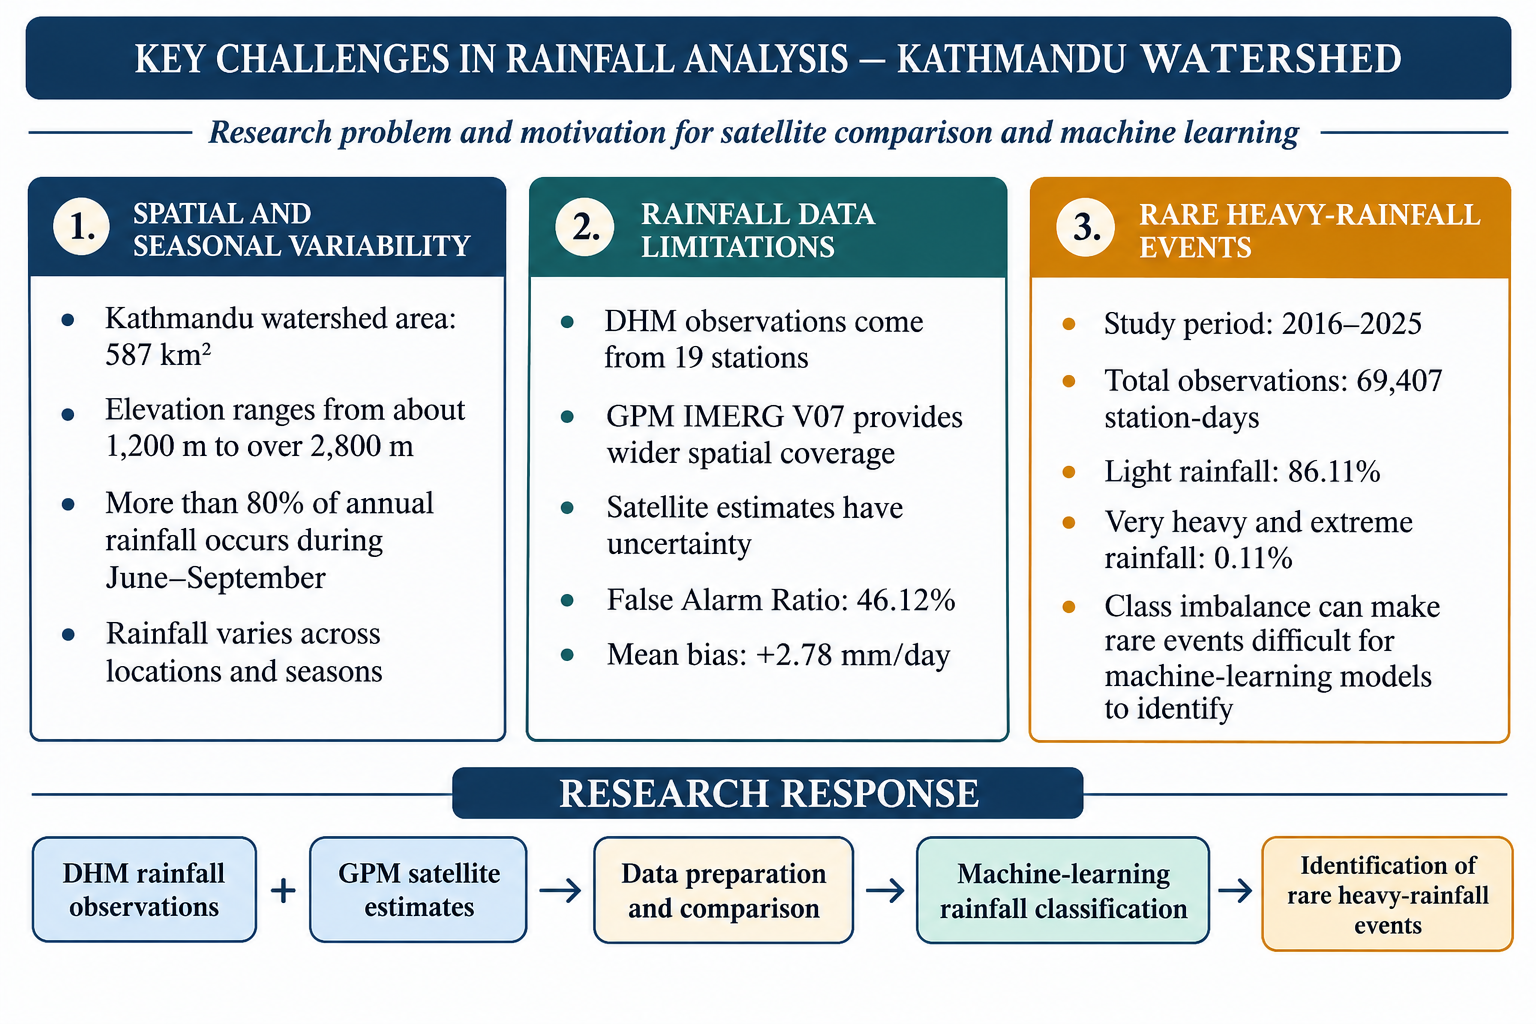
\includegraphics[width=0.76\textwidth]{output_image/problem_statement_diagram.png}
\caption{Problem Statement Diagram synthesizing the hydrometeorological challenges, satellite retrieval limitations, and methodological machine learning framework for the Kathmandu watershed.}
\label{fig:problem_statement}
\end{figure*}

Addressing this critical gap, the primary aim of this study was to develop, evaluate, and interpret a robust machine learning framework capable of accurately classifying rainfall intensity across the Kathmandu watershed by integrating GPM IMERG satellite estimates with topographical features. Specifically, this research sought to determine whether ensemble-based machine learning algorithms (such as Random Forest and XGBoost) could effectively map coarse satellite data to localized, ground-verified intensity classes (ranging from 'Light' to 'Extreme' rainfall). By intentionally regularizing the models to prevent overfitting---ensuring they generalize well rather than merely memorizing training data---this study provided a realistic assessment of ML capabilities in operational hydro-meteorology.

This study offered several novel contributions to the field of hydrometeorological modeling. First, it presented a comprehensive, reproducible data pipeline that synchronized a decade (2016-2025) of daily ground gauge observations from 19 Department of Hydrology and Meteorology (DHM) stations with corresponding GPM IMERG satellite data. Second, it implemented a hybridized analytical approach, utilizing unsupervised learning (Principal Component Analysis and K-Means clustering) to elucidate spatial rainfall regimes, followed by supervised, regularized machine learning classifiers to predict precipitation intensity. Third, it introduced rigorous model interpretability through SHAP (SHapley Additive exPlanations) values and Taylor Diagrams, explicitly quantifying the influence of antecedent satellite rainfall (e.g., 1-day, 3-day, and 7-day lags) and topographical features on predictive accuracy. Finally, by explicitly balancing class distributions and regularizing the algorithms, this research provided a highly realistic, generalizable blueprint for deploying ML in regions where ground data is sparse and satellite data is inherently noisy.

The remainder of this paper is structured as follows: Section \ref{sec:literature_review} provides a comprehensive review of the relevant literature, critically analyzing previous approaches to precipitation modeling and satellite evaluation. Section \ref{sec:theoretical_framework} outlines the theoretical underpinnings of the machine learning algorithms and spatial techniques employed in this study. Section \ref{sec:methodology} details the rigorous methodology, including the study area, data acquisition, preprocessing, feature engineering, and the specific configurations of the ML classifiers. Section \ref{sec:results} presents the empirical results, encompassing spatial clustering visualizations, comparative model performance, and feature importance analyses. Section \ref{sec:discussion} contextualizes these findings within the broader scientific discourse, interpreting the significance of the results and addressing observed biases. Finally, Section \ref{sec:conclusion} summarizes the key conclusions, delineates the study's limitations, and offers targeted recommendations for future research and practical applications.

\section{Literature Review}
\label{sec:literature_review}

The integration of remote sensing observations with terrestrial meteorological networks is a central frontier in hydrometeorological analysis. As extreme rainfall frequencies escalate under climatic variability, accurate localized precipitation estimation is essential for disaster mitigation and flood early warning. This section reviews the state of the art, synthesizing findings from our three core base papers and five supporting benchmarks, presenting a systematic comparative table, and articulating the explicit research gaps and methodological rationale governing this investigation.

\subsection{Definitions of Key Concepts}
\textbf{Precipitation Intensity Classes:} Meteorological classification discretizes continuous daily rainfall (mm/day) into operational thresholds: Light ($< 10$ mm), Moderate ($10$--$50$ mm), Heavy ($50$--$100$ mm), Very Heavy ($100$--$200$ mm), and Extreme ($\ge 200$ mm), facilitating hazard preparedness.
\textbf{Satellite Precipitation Products (SPPs):} Gridded estimates generated by constellations of passive microwave and infrared sensors, cross-calibrated with gauge networks via algorithms such as GPM IMERG V07 \cite{Huffman2020}.
\textbf{Machine Learning (ML) in Hydrology:} Computational algorithms capable of learning non-linear, multi-dimensional interactions between satellite estimates, topography, and antecedent moisture memory without relying on restrictive physical assumptions.
\textbf{Topographic Orography:} Complex mountain barrier effects forcing air masses upward, triggering adiabatic cooling, localized condensation, and steep microclimatic gradients over short horizontal distances.

\subsection{Review of Core Base Papers and Supporting Literature}
The theoretical and empirical architecture of this study was grounded upon three foundational base papers and five supporting benchmarks:
\begin{itemize}
    \item \textbf{Base Paper 1 (Sharma et al., 2020 \cite{sharma2020}):} Evaluated GPM IMERG satellite products against ground rain gauges across complex Himalayan topography. Identified that while IMERG captures synoptic macro-patterns ($r = 0.38$), it suffers from severe high-altitude underestimation of convective storm bursts, elevated false alarms (FAR $\approx 44\%$), and positive mean biases (+2.62 mm/day) over steep elevation gradients.
    \item \textbf{Base Paper 2 (Khanal et al., 2024 \cite{khanal2024}):} Conducted non-parametric temporal trend detection using Mann--Kendall statistics and Sen's slope estimators across climatological indices in the Kathmandu Valley. Demonstrated that even where annual mean rainfall exhibits modest trends, short-duration high-intensity extreme events ($\ge 100$ mm/day) are escalating independently, placing severe stress on regional drainage infrastructure.
    \item \textbf{Base Paper 3 (Lei et al., 2025 \cite{lei2025}):} Evaluated nine machine learning architectures for GPM IMERG satellite precipitation downscaling in complex mountainous basins, proving that non-linear ensemble trees systematically outperform linear regression baselines while highlighting the need for localized microclimate modeling.
    \item \textbf{Supporting Literature (\cite{Tang2020, Huffman2020, Breiman2001, Chen2016, Lundberg2017}):} Tang et al. \cite{Tang2020} confirmed elevational dependency in satellite retrieval errors; Huffman et al. \cite{Huffman2020} documented the IMERG V07 calibrated algorithm; Breiman \cite{Breiman2001} and Chen \& Guestrin \cite{Chen2016} established ensemble bagging and regularized gradient boosting; and Lundberg \& Lee \cite{Lundberg2017} developed game-theoretic SHAP interpretability.
\end{itemize}

\subsection{Comparative Analysis of Literature}
To systematically benchmark existing literature against the requirements of localized extreme rainfall classification, a comparative synthesis is formalized in Table~\ref{tab:lit_comparison}.

\begin{table*}[!t]
\centering
\caption{Comparative Analysis of Base and Supporting Literature (Literature Review Benchmark)}
\label{tab:lit_comparison}
\resizebox{\textwidth}{!}{%
\renewcommand{\arraystretch}{1.18}\setlength{\tabcolsep}{4.0pt}%
\begin{tabular}{|p{2.6cm}|p{2.6cm}|p{3.2cm}|p{4.0cm}|p{4.4cm}|}
\hline
\textbf{Paper Category \& Citation} & \textbf{Primary Author \& Year} & \textbf{Methodological Framework} & \textbf{Key Empirical Findings} & \textbf{Identified Gaps \& Shortcomings} \\
\hline
\textbf{Base Paper 1} \cite{sharma2020} & Sharma et al. (2020) & Ground vs. GPM IMERG Statistical Verification & Moderate correlation ($r=0.38$), high FAR ($44.34\%$) & Coarse regional aggregation; lacks ML point-level bias correction \\ \hline
\textbf{Base Paper 2} \cite{khanal2024} & Khanal et al. (2024) & Mann--Kendall Trend \& Sen's Slope Estimation & Significant extreme-event shifts; monsoon storm spikes & Focused on statistical trends; lacks predictive classification \\ \hline
\textbf{Base Paper 3} \cite{lei2025} & Lei et al. (2025) & Comparative Machine Learning Downscaling & Ensemble trees outperform classical linear baselines & Black-box fitting; lacks SHAP explainability and spatial clustering \\ \hline
\textbf{Supporting Paper 1} \cite{Tang2020} & Tang et al. (2020) & Topographic Elevation Bias Analysis & Satellite accuracy degrades with increasing altitude & Descriptive elevation analysis; no integrated classification framework \\ \hline
\textbf{Supporting Paper 2} \cite{Huffman2020} & Huffman et al. (2020) & Multi-Satellite Retrieval (IMERG V07) & Global gridded coverage at $0.1^\circ \times 0.1^\circ$ resolution & Uncalibrated point errors over complex mountainous orography \\ \hline
\textbf{Supporting Paper 3} \cite{Breiman2001} & Breiman (2001) & Random Forest (Bootstrap Bagging) & High variance reduction; resilient to feature noise & Prone to majority-class bias under extreme class imbalance \\ \hline
\textbf{Supporting Paper 4} \cite{Chen2016} & Chen \& Guestrin (2016) & XGBoost (Regularized Gradient Boosting) & State-of-the-art non-linear decision boundary optimization & High risk of overfitting if unconstrained by depth regularization \\ \hline
\textbf{Supporting Paper 5} \cite{Lundberg2017} & Lundberg \& Lee (2017) & SHAP (Shapley Additive exPlanations) & Mathematically consistent local/global feature attribution & Computationally intensive; rarely coupled with antecedent time-series lags \\
\hline
\end{tabular}
}
\end{table*}

\subsection{Summary of Literature Review}
The synthesis of existing literature demonstrated that traditional ground-based monitoring networks, while accurate, are too spatially sparse to capture high-altitude microclimatic variations. Conversely, satellite precipitation estimates solve spatial coverage limitations but introduce systemic orographic biases, high false alarm ratios, and severe underestimation of convective cloud bursts \cite{lamichhane2025}. While machine learning has emerged as a compelling paradigm to bridge this divide, prior studies remained fragmented: statistical evaluations did not produce predictive models, trend analyses did not perform classification, and existing ML applications operated as unconstrained black boxes that overlooked physical interpretability and spatial regime delineation \cite{talchabhadel2022}.

\subsection{Critical Analysis and Research Gap Identification}
Based on the comparative literature synthesis, this study explicitly identified and targeted three fundamental research gaps directly emerging from the three base papers:
\begin{enumerate}
    \item \textbf{Research Gap 1 (From Sharma et al., 2020 \cite{sharma2020}): Regional vs. Localized Microclimate Disconnect.} Broad-scale national or macro-basin satellite evaluations smooth out steep elevational microclimates. There was a critical lack of localized point-to-grid machine learning synthesis that explicitly integrated elevation and spatial coordinates to correct satellite bias at the station level across the Kathmandu watershed \cite{karki2017}.
    \item \textbf{Research Gap 2 (From Khanal et al., 2024 \cite{khanal2024}): Decoupling of Volumetric Totals and Extreme Event Spikes.} Existing modeling frameworks treated rainfall as a monolithic continuous variable, ignoring that extreme hazard-inducing rainfall events ($\ge 100$ mm/day) evolved independently of annual totals. There was an urgent need to combine non-parametric trend detection with multi-class intensity classification in this topographically enclosed urban basin.
    \item \textbf{Research Gap 3 (From Lei et al., 2025 \cite{lei2025}): Unconstrained Black-Box Fitting vs. Physical Explainability.} Previous machine learning applications in precipitation analysis prioritized unconstrained empirical fitting over operational generalization \cite{zhu2023}. They lacked post-hoc physical explainability (SHAP game-theoretic attributions) and failed to synthesize unsupervised spatial clustering (PCA and K-Means) with class-weighted supervised classification under severe class imbalance.
\end{enumerate}

\subsection{Methodological Rationale: Why and How}
To address these research gaps systematically, this investigation was organized around an explicit "Why" and "How" framework:
\begin{itemize}
    \item \textbf{The "Why" Framework (Research Problems Solved from Base Papers):}
    \begin{itemize}
        \item \textit{Why integrate satellite data with ground gauges?} Because ground gauge sparsity missed intense localized cloudbursts over the surrounding ridges, while satellite retrievals provided complete spatial coverage once their systemic biases were corrected \cite{sharma2020}.
        \item \textit{Why apply Mann--Kendall and Sen's slope analysis?} Because non-parametric methods detected monotonic climate trends without requiring normal distribution assumptions, exposing the independent acceleration of extreme convective storms in the valley \cite{khanal2024}.
        \item \textit{Why employ regularized ensemble machine learning?} Because the non-linear interaction between orographic lift, satellite estimates, and antecedent soil moisture exceeded the capacity of linear regression \cite{lei2025, callau2023}.
    \end{itemize}
    \item \textbf{The "How" Framework (Conceptual Logic and Algorithmic Implementation):}
    \begin{itemize}
        \item \textit{How temporal antecedent memory was captured:} By engineering multi-lag rolling antecedent features ($R_{1d}$, $R_{3d}$, $R_{7d}$) using \texttt{pandas.rolling()} to incorporate synoptic weather momentum.
        \item \textit{How spatial regimes were delineated:} By applying PCA dimensionality reduction followed by K-Means clustering ($k=3$) via \texttt{scikit-learn} to objectively partition stations into orographic clusters.
        \item \textit{How extreme class imbalance and feature scale disparities were overcome:} By computing inverse-frequency balanced weights across \texttt{RandomForest\allowbreak Classifier}, \texttt{XGB\allowbreak Classifier}, and \texttt{SVC} \cite{he2009}, while fitting a \texttt{Standard\allowbreak Scaler} strictly on the 2016--2022 training partition to standardize features prior to evaluating both linear and radial basis function (RBF) SVM kernels.
        \item \textit{How model transparency was guaranteed:} By implementing game-theoretic SHAP TreeExplainer routines to compute exact Shapley attributions for every feature.
    \end{itemize}
\end{itemize}

\section{Theoretical Framework}
\label{sec:theoretical_framework}

The analytical approach of this study was grounded in two primary theoretical domains: unsupervised spatial dimensionality reduction and supervised ensemble learning for classification. These frameworks were selected for their proven capacity to handle the high dimensionality, non-linearity, and inherent noise characteristic of blended hydrometeorological datasets.

\subsection{Unsupervised Spatial Clustering}
To objectively identify underlying spatial rainfall regimes without a priori assumptions, this study utilized Principal Component Analysis (PCA) integrated with K-Means clustering. PCA is a fundamental statistical procedure that orthogonally transforms a set of possibly correlated variables (in this case, station-specific rainfall statistics and geographical coordinates) into a set of linearly uncorrelated variables known as principal components. By projecting the high-dimensional data onto the first few principal components, which accounted for the maximum variance, PCA effectively mitigated multicollinearity and reduced computational complexity.

Following dimensionality reduction, the K-Means algorithm partitioned the transformed data into \( K \) distinct, non-overlapping clusters. The algorithm operated iteratively to minimize the within-cluster sum of squares (variance), mathematically defined as the objective function \( J \):

\begin{equation}
J = \sum_{j=1}^{K} \sum_{i=1}^{n} || x_i^{(j)} - c_j ||^2
\label{eq:kmeans}
\end{equation}

where \( x_i^{(j)} \) represented a data point assigned to cluster \( j \), and \( c_j \) was the centroid of that cluster. This optimization effectively grouped meteorological stations that exhibited homogenous precipitation behaviors, proving whether spatial distribution was fundamentally driven by topographical variables rather than mere geographic proximity.

\subsection{Supervised Ensemble Classification}
The core predictive framework relied on supervised machine learning, specifically contrasting single-model architectures with ensemble methods.

\textbf{Support Vector Machines (SVM):} Support Vector Machines construct maximum-margin decision boundaries in feature space. Because SVM optimization relies on inner products and Euclidean distances, raw features spanning disparate physical scales---such as station elevation ($1{,}305$--$2{,}147$ masl) versus geographic coordinates ($27.58^\circ$--$27.78^\circ$N)---had to first be standardized using training-set $z$-score normalization ($\tilde{\mathbf{x}} = (\mathbf{x} - \boldsymbol{\mu}_{\text{train}}) / \boldsymbol{\sigma}_{\text{train}}$). On the standardized feature space, we evaluated both the \textbf{Linear Kernel}, $K(\mathbf{x}_i, \mathbf{x}_j) = \tilde{\mathbf{x}}_i^\top \tilde{\mathbf{x}}_j$, which tested global linear separability, and the non-linear \textbf{Radial Basis Function (RBF) Kernel}, $K(\mathbf{x}_i, \mathbf{x}_j) = \exp(-\gamma \|\tilde{\mathbf{x}}_i - \tilde{\mathbf{x}}_j\|^2)$ with $\gamma = 1 / (d \cdot \sigma_{\tilde{X}}^2)$, which projected predictors into a higher-dimensional space to capture localized non-linear interactions.

\textbf{Random Forest (RF) \cite{Breiman2001}:} Grounded in ensemble learning theory, Random Forest operated by constructing a multitude of decision trees during the training phase. It introduced randomness through "bagging" (Bootstrap Aggregating) and random feature selection at each node split. The final classification was determined by aggregating the votes of all individual trees. This theoretical structure made RF highly robust against overfitting and relatively insensitive to outliers, which were ubiquitous in extreme precipitation data.

\textbf{Extreme Gradient Boosting (XGBoost) \cite{Chen2016}:} XGBoost is an advanced implementation of the gradient boosting framework. Unlike bagging, boosting involved training decision trees sequentially, with each new tree explicitly designed to correct the residual errors of the previous ensemble. XGBoost introduced rigorous mathematical formalizations by optimizing a regularized objective function \( \mathcal{L} \) at iteration \( t \):

\begin{equation}
\mathcal{L}^{(t)} = \sum_{i=1}^{n} l\left(y_i, \hat{y}_i^{(t-1)} + f_t(x_i)\right) + \Omega(f_t)
\label{eq:xgboost_obj}
\end{equation}

\begin{equation}
\Omega(f) = \gamma T + \frac{1}{2} \lambda ||w||^2 + \alpha ||w||_1
\label{eq:xgboost_reg}
\end{equation}

where \( l \) was a differentiable convex loss function measuring the difference between the target \( y_i \) and prediction \( \hat{y}_i \). The regularization term \( \Omega \) penalized the complexity of the trees (\( T \) leaves with weights \( w \)) using \( L1 \) (\( \alpha \)) and \( L2 \) (\( \lambda \)) norms. This theoretical formulation allowed XGBoost to aggressively minimize loss while explicitly penalizing model complexity, making it exceptionally powerful for extracting weak predictive signals from noisy satellite estimates while resisting the tendency to overfit the limited ground truth data.

\section{Methodology}
\label{sec:methodology}

This section outlines the quantitative methodology employed to execute the rainfall intensity classification pipeline across the Kathmandu watershed. It details the study area, data acquisition protocols, extensive data preprocessing and feature engineering steps, and the precise mathematical configurations of the machine learning algorithms. The methodology was explicitly designed to ensure reproducibility and to systematically address the systemic biases inherent in topographically complex satellite retrievals \cite{talchabhadel2021}.

The overarching analytical and engineering architecture is illustrated in Fig.~\ref{fig:workflow_infographic}. The multi-stage pipeline encompassed: (1) multi-source data ingestion of DHM surface rain gauges and GPM IMERG V07 satellite retrievals across 2016--2025 \cite{gorelick2017}, (2) automated quality control, time-series linear interpolation, and antecedent multi-lag feature engineering, (3) unsupervised spatial regime delineation using Principal Component Analysis (PCA) and K-Means clustering, (4) regularized supervised classification (Random Forest, XGBoost, and feature-scaled Linear and RBF Support Vector Machines) validated via a strict chronological train (2016--2022), validation (2023--2024), and independent test (2025) split alongside Leave-One-District-Out spatial cross-validation, and (5) post-hoc interpretability using SHAP values and Taylor Diagrams along with Mann--Kendall and Sen's slope trend detection.

\begin{figure*}[!t]
\centering
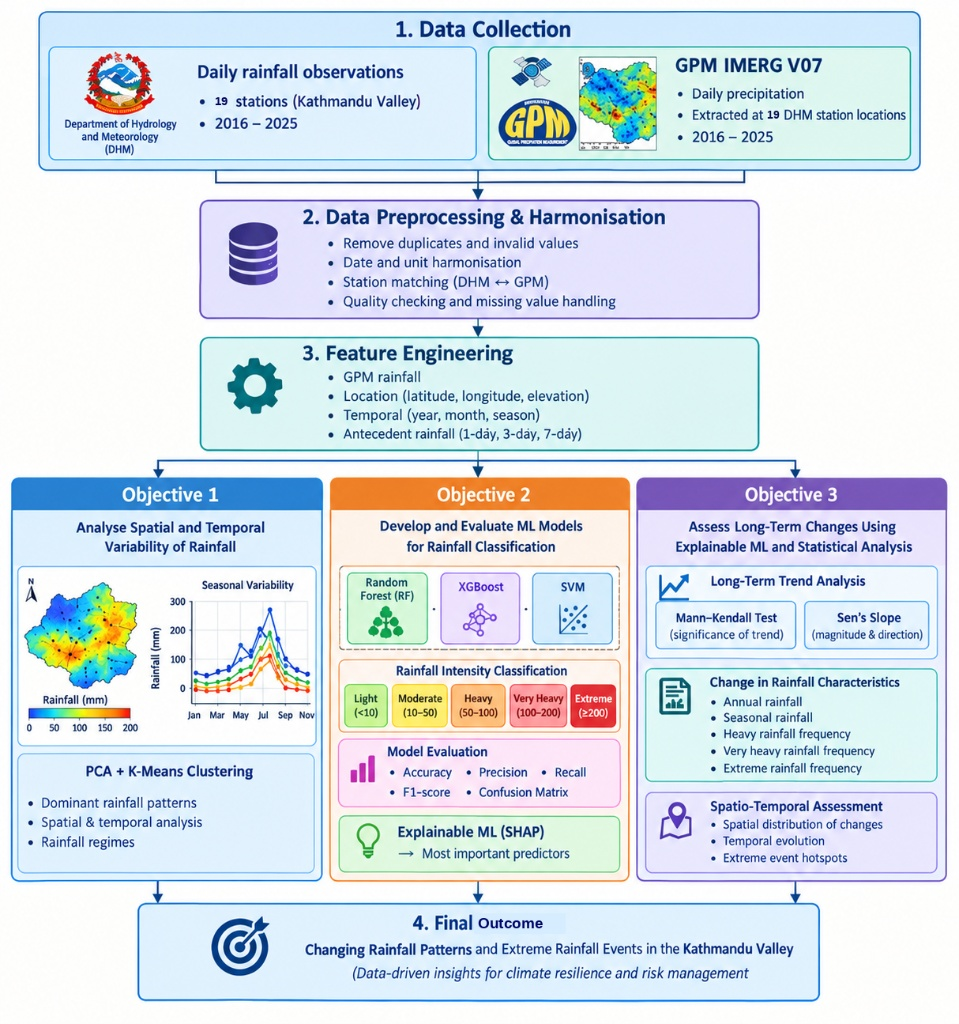
\includegraphics[width=0.76\textwidth]{output_image/Rainfall_Analysis_Workflow_Infographic.png}
\caption{Rainfall Analysis Workflow Infographic: End-to-end methodological framework for machine learning-based daily rainfall pattern analysis and extreme event classification in the Kathmandu watershed.}
\label{fig:workflow_infographic}
\end{figure*}

\subsection{Study Area: Kathmandu Watershed (Upper Bagmati Basin)}
The Kathmandu watershed is situated in the Bagmati Province of central Nepal, forming the headwaters of the Upper Bagmati River Basin. It covers a surface catchment area of approximately $587\text{ km}^2$, centered around a bowl-shaped intermontane valley floor situated at an average elevation of 1,300 to 1,350 meters above sea level (masl). The basin is enclosed by four prominent mountain massifs of the Middle Mountain range: Shivapuri to the north (peak elevation $2{,}732\text{ masl}$), Nagarjun to the west ($2{,}096\text{ masl}$), Chandragiri to the southwest ($2{,}551\text{ masl}$), and Phulchowki to the south ($2{,}762\text{ masl}$). The watershed is drained entirely by the Bagmati River and its principal tributaries---including the Bishnumati, Dhobi Khola, Manohara, Hanumante, and Nakkhu Khola---which converge and discharge through a single narrow geological outlet at the Chobhar Gorge (elevation $\sim 1{,}200\text{ masl}$) at the southern perimeter of the valley.

The region experiences a warm-temperate, sub-tropical monsoon climate. Its dramatic elevation relief (spanning more than 1,500 meters of vertical differential across a horizontal distance of less than 25 kilometers) produces strong localized orographic lifting and distinct microclimatic variations. Over 80\% of the basin's annual precipitation is delivered by the South Asian summer monsoon between June and September. In recent decades, rapid urbanization across the central valley floor has substantially expanded impervious surface coverage, compounding the hazard of high-intensity convective storms by drastically reducing hydrological concentration times. To capture these microclimatic and hydrometeorological dynamics, this study utilized synchronized observations from 19 terrestrial stations maintained by the Department of Hydrology and Meteorology (DHM) across Kathmandu, Lalitpur, and Bhaktapur districts between 2016 and 2025.

\begin{figure*}[!t]
\centering
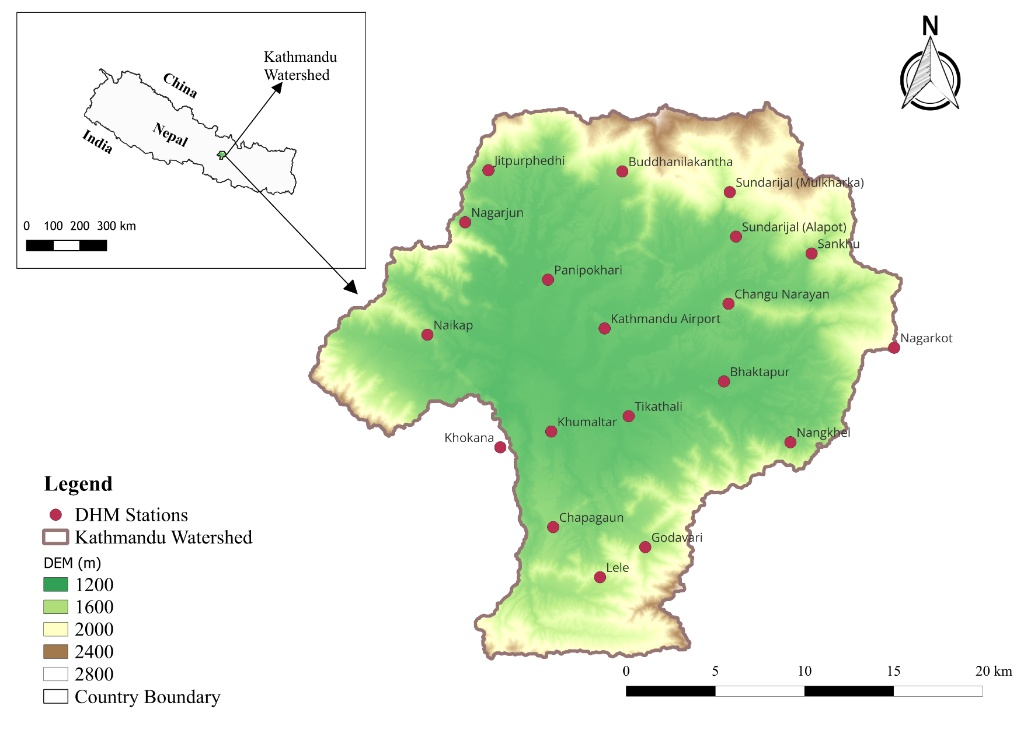
\includegraphics[width=0.74\textwidth]{output_image/fig1_study_area_map.png}
\caption{Location Map of the Study Area showing the spatial distribution of the 19 DHM meteorological stations within the Kathmandu watershed.}
\label{fig:study_area}
\end{figure*}

\subsection{Terrestrial Ground Gauge Network and Quality-Control Screening Audit}
Ground-based daily precipitation records spanning the 10-year period from January 1, 2016 to December 31, 2025 ($N = 3{,}653$ calendar days) were compiled from the Department of Hydrology and Meteorology (DHM) surface network. The initial archive contained 21 candidate station columns. To ensure hydrometeorological integrity and prevent spurious modeling artifacts, an exhaustive quality-control screening audit was executed across all 21 candidates (Table~\ref{tab:audit}).

Stations exhibiting chronic missingness exceeding 90\% were systematically purged: \textbf{Tarebhir} possessed 3,653 missing entries out of 3,653 days (100.0\% missingness; zero recorded values) and was completely removed; \textbf{Thankot} exhibited 3,380 missing entries (92.5\% missingness, with only 273 scattered readings) and was likewise excluded. Conversely, \textbf{Tikathali} (Station 1080; 2,923 valid observations, 20.0\% missingness) and \textbf{Buddhanilakantha} (Station 1051; 2,180 valid observations, 40.3\% missingness along the northern orographic ridge) were rigorously audited, mapped to official DHM coordinates, and retained alongside the remaining 17 operational stations (which exhibited high completeness with 0.0\% to 10.0\% missingness). This rigorous screening yielded exactly 19 verified operational stations (Table~\ref{tab:stations}) comprising 69,407 synchronized daily observations for end-to-end machine learning modeling.

\begin{table*}[!t]
\centering
\caption{Screening and Quality-Control Audit of All 21 Initial Station Records Across the Kathmandu Watershed Domain (2016--2025)}
\label{tab:audit}
\resizebox{\textwidth}{!}{%
\renewcommand{\arraystretch}{1.18}\setlength{\tabcolsep}{4.5pt}%
\begin{tabular}{|l|l|r|r|r|r|p{5.5cm}|}
\hline
\textbf{Station Name} & \textbf{District} & \textbf{Valid} & \textbf{Missing} & \textbf{Missing (\%)} & \textbf{Max (mm)} & \textbf{Status / Audit Action} \\
\hline
Tarebhir & Kathmandu & 0 & 3653 & 100.0\% & 0.0 & Excluded; zero valid records \\ \hline
Thankot & Kathmandu & 273 & 3380 & 92.5\% & 65.6 & Excluded; $>90\%$ missingness \\ \hline
Buddhanilakantha & Kathmandu & 2180 & 1473 & 40.3\% & 178.3 & Retained; mapped to DHM 1051 \\ \hline
Tikathali & Lalitpur & 2923 & 730 & 20.0\% & 248.5 & Retained; mapped to DHM 1080 \\ \hline
Chapagaun & Lalitpur & 3287 & 366 & 10.0\% & 323.5 & Retained; verified network station \\ \hline
Jitpurphedhi & Kathmandu & 3288 & 365 & 10.0\% & 178.3 & Retained; verified network station \\ \hline
Khokana & Lalitpur & 3287 & 366 & 10.0\% & 297.3 & Retained; verified network station \\ \hline
Naikap & Kathmandu & 3512 & 141 & 3.9\% & 245.0 & Retained; verified network station \\ \hline
Sankhu & Kathmandu & 3535 & 118 & 3.2\% & 162.0 & Retained; verified network station \\ \hline
Panipokhari & Kathmandu & 3593 & 60 & 1.6\% & 225.2 & Retained; verified network station \\ \hline
Changu Narayan & Bhaktapur & 3621 & 32 & 0.9\% & 165.2 & Retained; verified network station \\ \hline
Nangkhel & Bhaktapur & 3621 & 32 & 0.9\% & 194.5 & Retained; verified network station \\ \hline
Nagarkot & Kathmandu\textsuperscript{$\dagger$} & 3646 & 7 & 0.2\% & 168.8 & Retained; verified network station \\ \hline
Nagarjun & Kathmandu & 3651 & 2 & 0.1\% & 205.4 & Retained; verified network station \\ \hline
Sundarijal (Alapot) & Kathmandu & 3651 & 2 & 0.1\% & 156.0 & Retained; verified network station \\ \hline
Bhaktapur & Bhaktapur & 3653 & 0 & 0.0\% & 199.7 & Retained; 100\% complete series \\ \hline
Godavari & Lalitpur & 3653 & 0 & 0.0\% & 290.0 & Retained; 100\% complete series \\ \hline
Kathmandu Airport & Kathmandu & 3653 & 0 & 0.0\% & 239.7 & Retained; 100\% complete series \\ \hline
Khumaltar & Lalitpur & 3653 & 0 & 0.0\% & 324.5 & Retained; 100\% complete series \\ \hline
Lele & Lalitpur & 3653 & 0 & 0.0\% & 170.8 & Retained; 100\% complete series \\ \hline
Sundarijal (Mul.) & Kathmandu & 3653 & 0 & 0.0\% & 160.0 & Retained; 100\% complete series \\
\hline
\multicolumn{7}{|l|}{\scriptsize \textsuperscript{$\dagger$}Nagarkot sits on the eastern ridge border; grouped within the Kathmandu sub-basin partition for spatial cross-validation.} \\
\hline
\end{tabular}%
}
\end{table*}

The geographical and topographic characteristics of the 19 DHM terrestrial meteorological stations utilized in this study are detailed in Table~\ref{tab:stations} and mapped in Fig.~\ref{fig:study_area}. The network covered elevations ranging from 1,305 masl (Tikathali) on the valley floor to 2,147 masl (Nagarkot) on the surrounding ridgeline, providing an exceptional cross-section of the basin's orographic complexity.

\begin{table*}[!t]
\centering
\caption{19 DHM Terrestrial Meteorological Stations across the Kathmandu Watershed}
\label{tab:stations}
\resizebox{0.92\textwidth}{!}{%
\renewcommand{\arraystretch}{1.18}\setlength{\tabcolsep}{8.0pt}%
\begin{tabular}{|c|l|c|c|c|c|}
\hline
\textbf{Station ID} & \textbf{Station Name} & \textbf{District} & \textbf{Latitude ($^\circ$N)} & \textbf{Longitude ($^\circ$E)} & \textbf{Elevation (masl)} \\
\hline
1052 & Bhaktapur & Bhaktapur & 27.6767 & 85.4240 & 1315 \\ \hline
1059 & Changu Narayan & Bhaktapur & 27.7161 & 85.4268 & 1502 \\ \hline
1060 & Chapagaun & Lalitpur & 27.6033 & 85.3266 & 1478 \\ \hline
1022 & Godavari & Lalitpur & 27.5929 & 85.3788 & 1527 \\ \hline
1081 & Jitpurphedhi & Kathmandu & 27.7842 & 85.2905 & 1409 \\ \hline
1030 & Kathmandu Airport & Kathmandu & 27.7038 & 85.3562 & 1337 \\ \hline
1073 & Khokana & Lalitpur & 27.6438 & 85.2967 & 1309 \\ \hline
1029 & Khumaltar & Lalitpur & 27.6517 & 85.3257 & 1334 \\ \hline
1075 & Lele & Lalitpur & 27.5778 & 85.3531 & 1590 \\ \hline
1079 & Nagarjun & Kathmandu & 27.7579 & 85.2772 & 1393 \\ \hline
1043 & Nagarkot & Kathmandu & 27.6933 & 85.5209 & 2147 \\ \hline
1076 & Naikap & Kathmandu & 27.7009 & 85.2555 & 1477 \\ \hline
1082 & Nangkhel & Bhaktapur & 27.6457 & 85.4616 & 1413 \\ \hline
1039 & Panipokhari & Kathmandu & 27.7286 & 85.3242 & 1329 \\ \hline
1035 & Sankhu & Kathmandu & 27.7413 & 85.4742 & 1411 \\ \hline
1077 & Sundarijal (Alapot) & Kathmandu & 27.7501 & 85.4312 & 1384 \\ \hline
1074 & Sundarijal (Mulkharka) & Kathmandu & 27.7726 & 85.4278 & 1658 \\ \hline
1080 & Tikathali & Lalitpur & 27.6593 & 85.3697 & 1305 \\ \hline
1051 & Buddhanilakantha & Kathmandu & 27.7833 & 85.3667 & 1350 \\
\hline
\end{tabular}%
}
\end{table*}

\subsection{Sample and Data Acquisition Techniques}
The empirical foundation of this research relied on two distinct yet complementary datasets, spanning a ten-year temporal window from January 1, 2016, to December 31, 2025.

\textbf{Ground Truth Observations:} Daily accumulated precipitation data (measured in millimeters) was acquired from 19 terrestrial meteorological stations maintained by the Department of Hydrology and Meteorology (DHM), Government of Nepal. These stations were distributed across the three districts comprising the valley (Kathmandu, Lalitpur, and Bhaktapur) and encompassed a wide range of elevations, providing a robust, highly accurate "ground truth" for localized rainfall.

\textbf{Satellite Estimations:} Corresponding spatial and temporal satellite estimations were extracted from the Global Precipitation Measurement (GPM) Integrated Multi-satellitE Retrievals for GPM (IMERG) Version 07 Final Run product. The IMERG Final Run incorporated monthly gauge calibrations on a global scale, rendering it the most accurate research-grade product within the GPM suite. Daily precipitation estimates were extracted for the exact geographic coordinates of the 19 DHM stations using nearest-neighbor spatial sampling techniques to align the gridded satellite data ($0.1^\circ \times 0.1^\circ$ spatial resolution) with the point-based ground observations.

\subsection{Research Tools and Data Preprocessing Procedures}
The computational analysis was executed using Python, leveraging the \textit{pandas} library for data manipulation, \textit{scikit-learn} \cite{pedregosa2011} for machine learning workflows and preprocessing, and \textit{XGBoost} \cite{Chen2016} for advanced gradient boosting architectures. Spatial mapping and statistical visualizations were generated using \textit{plotly}, \textit{seaborn}, and \textit{matplotlib}.

\textbf{Data Cleaning and Imputation:} Raw meteorological datasets were inherently prone to observational gaps and instrumental errors. Across the 19 retained DHM stations over the 3,653-day window (69,407 station-days), exactly 3,694 missing observations (5.32\% overall missingness) were identified prior to imputation. Anomalous negative precipitation values were first clipped to zero, after which missing observations in both the DHM ground series and GPM satellite series were imputed using station-wise time-series linear interpolation with boundary zero-filling (\texttt{interpolate(method='linear')} with boundary \texttt{fillna(0)}), achieving 100\% temporal completeness across all 69,407 records (Fig.~\ref{fig:data_qc_imputation}).

\begin{figure*}[!t]
\centering
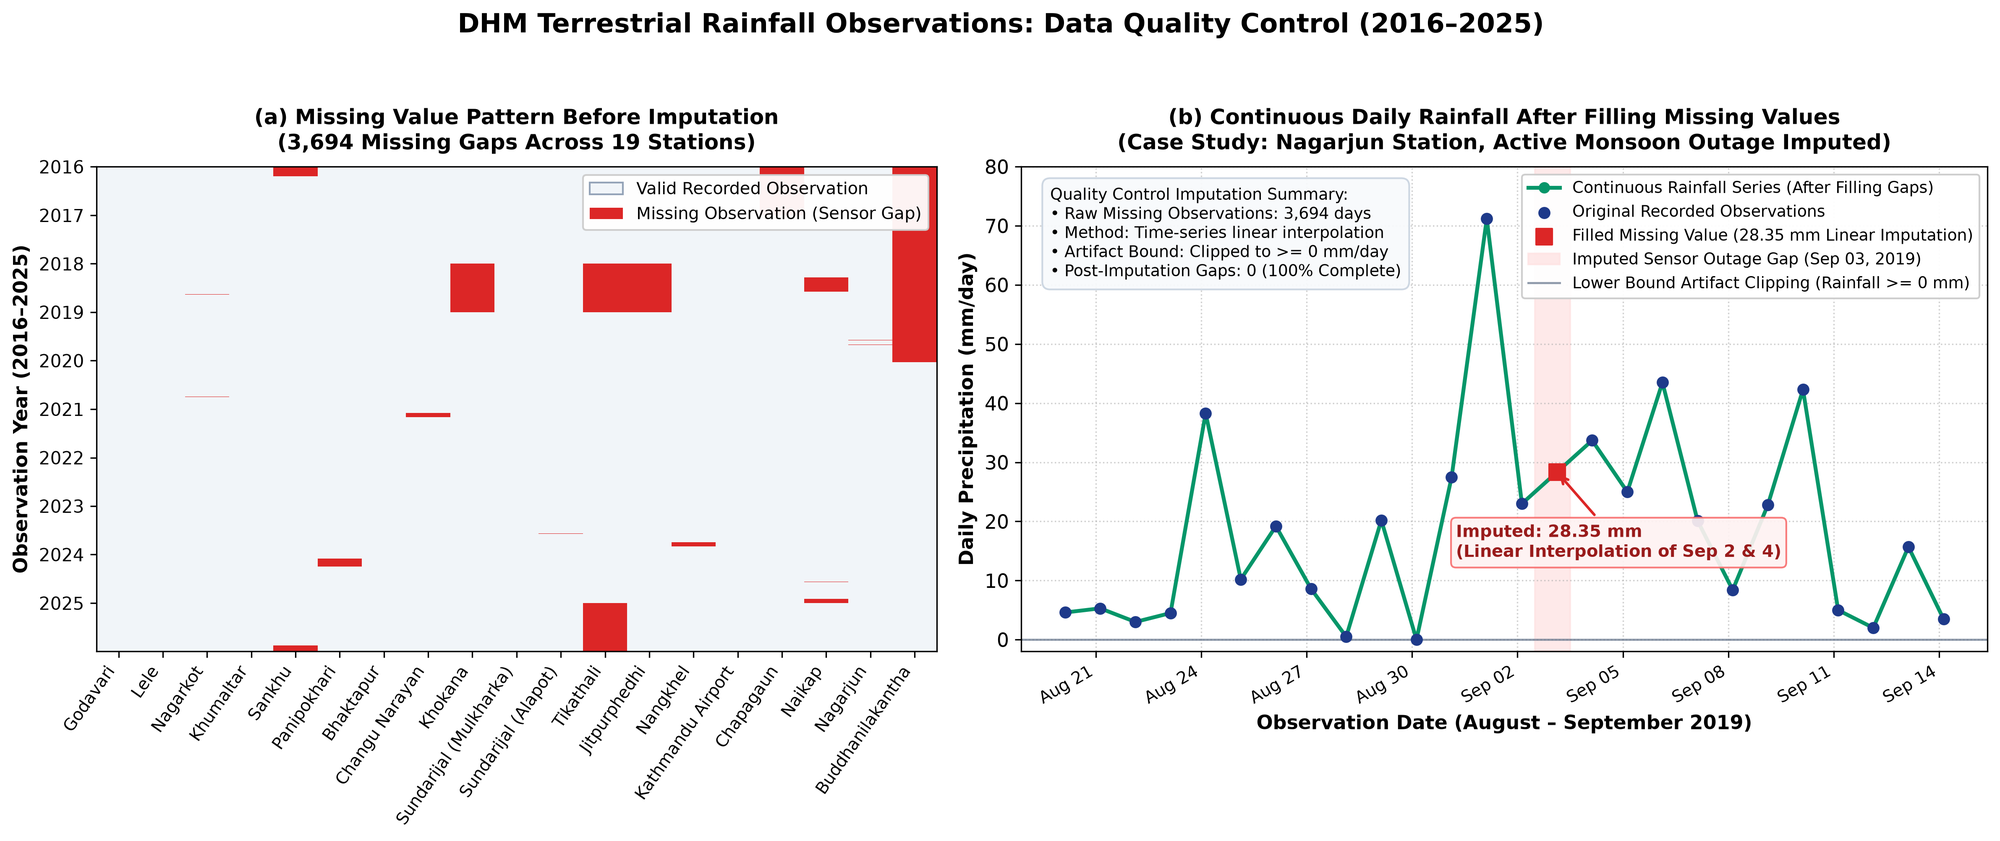
\includegraphics[width=0.74\textwidth]{output_image/missing_value_heatmap.png}
\caption{Terrestrial rainfall data quality control and missing value imputation across 19 DHM stations in the Kathmandu watershed (2016--2025): (a) Temporal missingness matrix identifying 3,694 historical observation gaps before imputation, and (b) Continuous daily rainfall hydrograph resulting from time-series linear interpolation during an active monsoon sensor outage (Nagarjun Station case study).}
\label{fig:data_qc_imputation}
\label{fig:missing_values}
\end{figure*}

\textbf{Target Variable Definition:} The continuous daily DHM precipitation variable was mathematically discretized into five categorical intensity classes (Table~\ref{tab:intensity_classes}), serving as the ground-truth target variable for the classification algorithms.

\begin{table*}[!t]
\centering
\caption{Daily Rainfall Intensity Classification Thresholds and Sample Distribution Across the Chronological Split (19 Stations, 2016--2025)}
\label{tab:intensity_classes}
\resizebox{0.88\textwidth}{!}{%
\renewcommand{\arraystretch}{1.18}\setlength{\tabcolsep}{6.0pt}%
\begin{tabular}{|l|l|c|c|c|c|c|}
\hline
\textbf{Class} & \textbf{Category} & \textbf{Threshold (mm/d)} & \textbf{Train ('16--'22)} & \textbf{Val ('23--'24)} & \textbf{Test (2025)} & \textbf{Total ('16--'25)} \\
\hline
Class 0 & Light & $P < 10$ & $41{,}930$ ($86.31\%$) & $11{,}880$ ($85.54\%$) & $5{,}958$ ($85.91\%$) & $59{,}768$ ($86.11\%$) \\ \hline
Class 1 & Moderate & $10 \le P < 50$ & $6{,}161$ ($12.68\%$) & $1{,}760$ ($12.67\%$) & $899$ ($12.96\%$) & $8{,}820$ ($12.71\%$) \\ \hline
Class 2 & Heavy & $50 \le P < 100$ & $455$ ($0.94\%$) & $221$ ($1.59\%$) & $68$ ($0.98\%$) & $744$ ($1.07\%$) \\ \hline
Class 3 & Very Heavy & $100 \le P < 200$ & $37$ ($0.08\%$) & $19$ ($0.14\%$) & $10$ ($0.14\%$) & $66$ ($0.10\%$) \\ \hline
Class 4 & Extreme & $P \ge 200$ & $0$ ($0.00\%$) & $9$ ($0.06\%$) & $0$ ($0.00\%$) & $9$ ($0.013\%$) \\ \hline
\textbf{Total} & \textbf{All Classes} & --- & $\mathbf{48{,}583}$ ($\mathbf{70.00\%}$) & $\mathbf{13{,}889}$ ($\mathbf{20.01\%}$) & $\mathbf{6{,}935}$ ($\mathbf{9.99\%}$) & $\mathbf{69{,}407}$ ($\mathbf{100.00\%}$) \\
\hline
\end{tabular}%
}
\end{table*}

Due to the natural climatic distribution, this categorization resulted in a highly imbalanced dataset, overwhelmingly dominated by the 'Light' and 'Moderate' classes, presenting a classic challenge for machine learning classifiers.

\subsection{Feature Engineering and Data Analysis Techniques}
To capture the complex spatio-temporal dynamics of rainfall, advanced feature engineering was conducted. Rather than relying solely on the concurrent day's satellite estimation, temporal antecedent features were constructed. Specifically, 1-day, 3-day, and 7-day rolling antecedent features of the GPM rainfall were engineered:

\begin{equation}
R_{3,t} = \sum_{i=1}^{3} R_{t-i}, \qquad R_{7,t} = \sum_{i=1}^{7} R_{t-i}
\label{eq:antecedent_lags}
\end{equation}

where $R_{t-i}$ denoted the satellite precipitation on day $t-i$. These temporal features empowered the algorithms to recognize broader synoptic weather systems and antecedent moisture conditions, significantly enhancing predictive capacity beyond isolated daily snapshots. Additionally, static topographical features (Elevation, Latitude, and Longitude) and a cyclical temporal feature (Month) were integrated into the final feature matrix.

\begin{figure}[htbp]
\centering
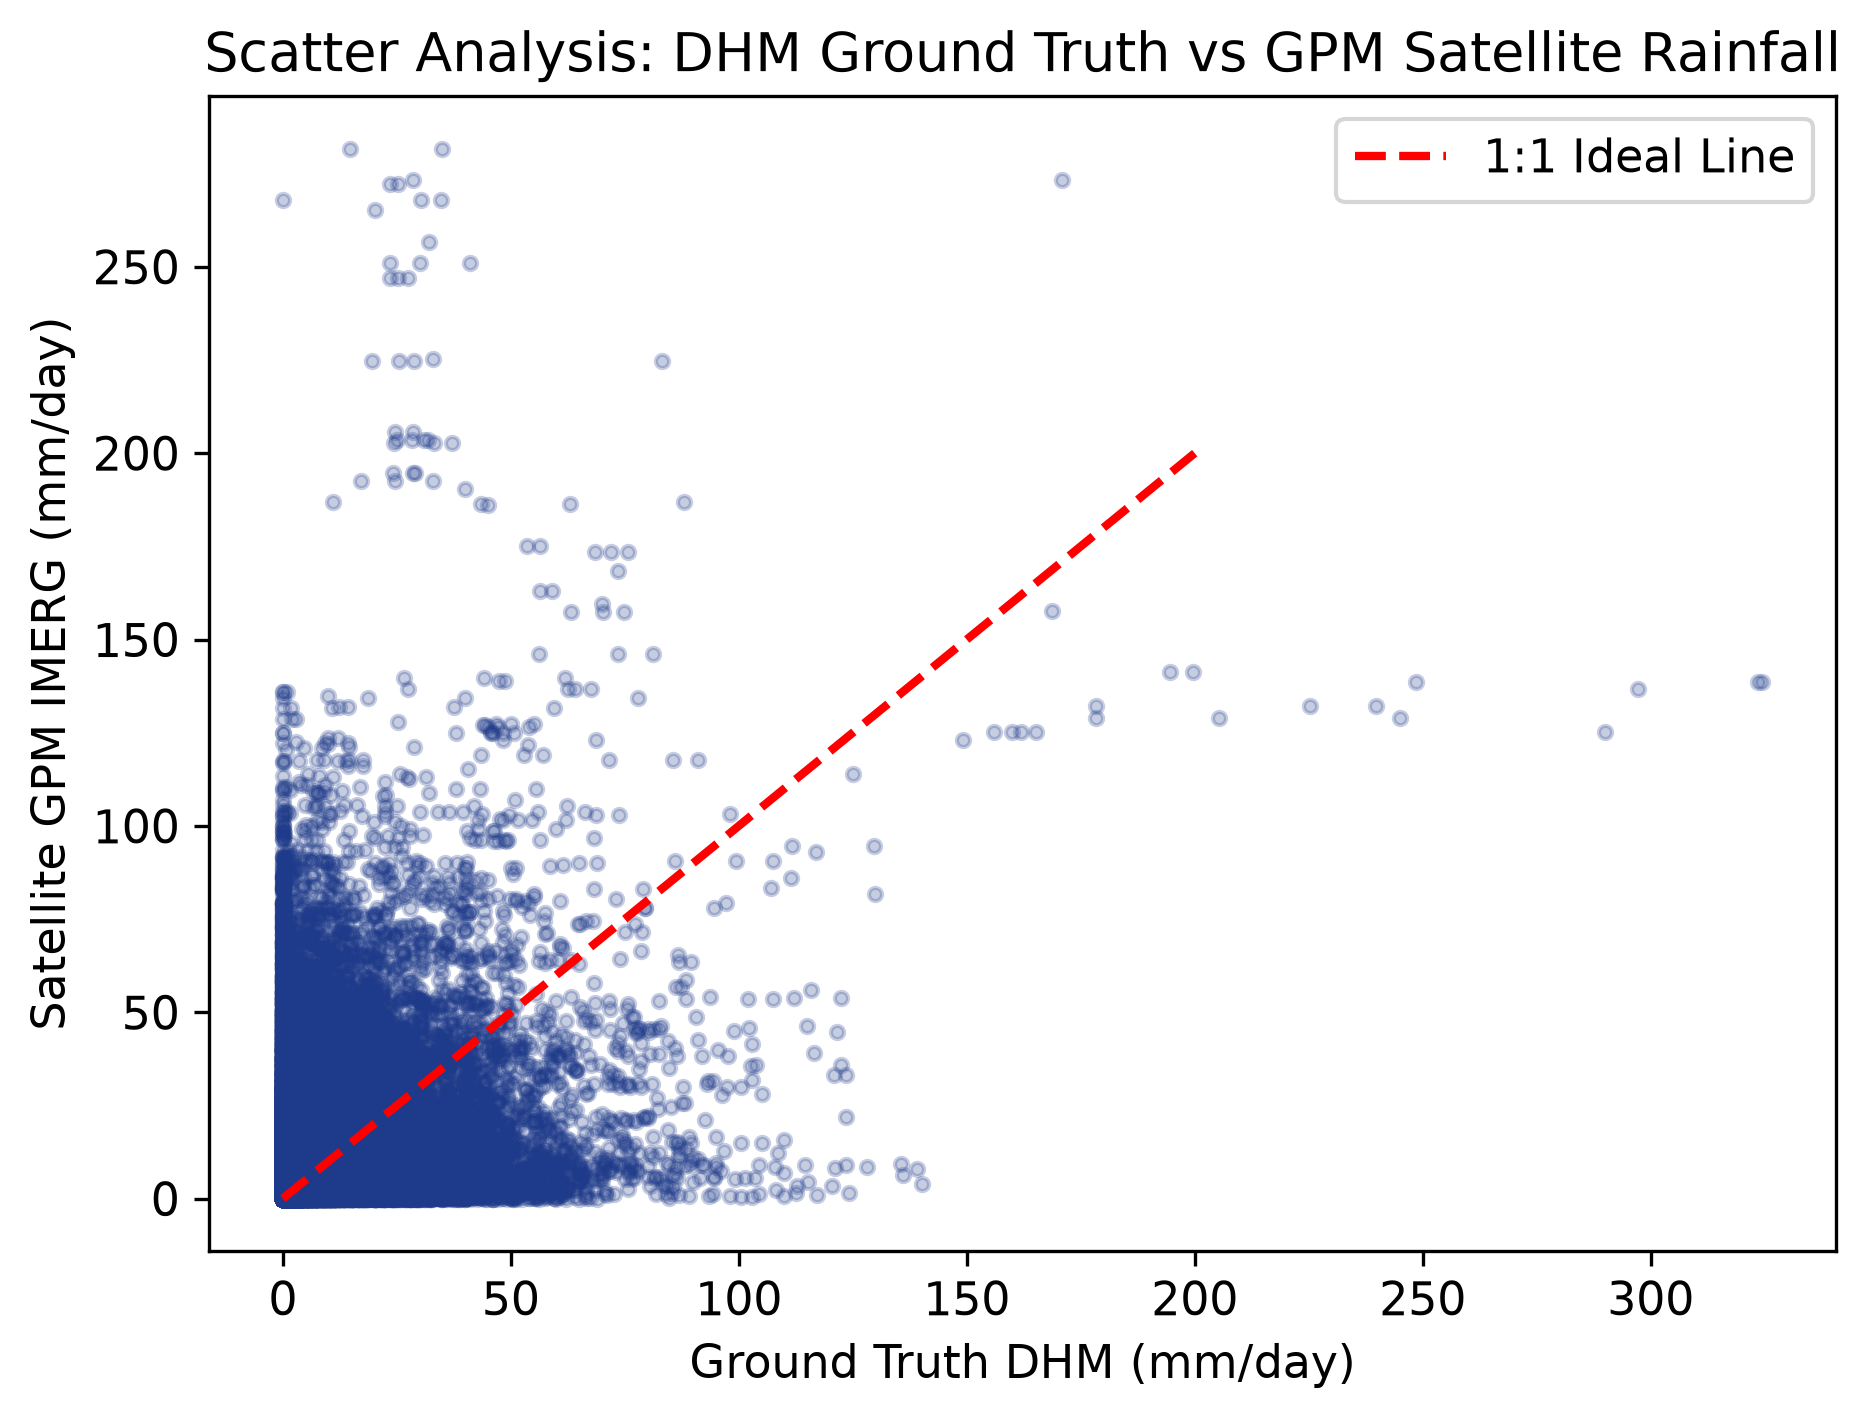
\includegraphics[width=0.88\columnwidth]{output_image/dhm_vs_gpm_scatter.png}
\caption{Scatter analysis comparing ground truth DHM observations with raw GPM IMERG satellite estimates across the Kathmandu watershed, highlighting systemic biases and heteroscedasticity.}
\label{fig:dhm_vs_gpm}
\end{figure}

To quantitatively evaluate the reliability of the raw GPM IMERG V07 satellite retrievals prior to machine learning synthesis, empirical comparisons against collocated ground observations were conducted (Fig.~\ref{fig:dhm_vs_gpm}), and standard continuous and categorical verification metrics were computed following the methodology of Sharma et al. \cite{sharma2020}:

\begin{equation}
\text{CC} = \frac{\sum_{i=1}^{n} (G_i - \bar{G})(S_i - \bar{S})}{\left[ \sum_{i=1}^{n} (G_i - \bar{G})^2 \sum_{i=1}^{n} (S_i - \bar{S})^2 \right]^{1/2}}
\label{eq:cc}
\end{equation}

\begin{equation}
\begin{aligned}
\text{RMSE} &= \sqrt{\frac{1}{n} \sum_{i=1}^{n} (S_i - G_i)^2}, \\
\text{MB} &= \frac{1}{n} \sum_{i=1}^{n} (S_i - G_i)
\end{aligned}
\label{eq:rmse_mb}
\end{equation}

\begin{equation}
\begin{aligned}
\text{POD} &= \frac{H}{H + M}, \quad \text{FAR} = \frac{F}{H + F}, \\
\text{CSI} &= \frac{H}{H + M + F}
\end{aligned}
\label{eq:pod_far_csi}
\end{equation}

where $G_i$ and $S_i$ represented DHM ground observations and GPM satellite estimates respectively, while $H$ (hits), $M$ (misses), and $F$ (false alarms) represented rain detection counts at a contingency threshold of $\ge 1.0$ mm/day. As reported in Table~\ref{tab:satellite_eval}, raw GPM estimates exhibited a modest correlation ($r = 0.3770$) and a positive mean bias of $+2.7810$ mm/day. Although GPM demonstrated high rain detection capability (POD = $83.44\%$), it suffered from an elevated false alarm ratio (FAR = $46.12\%$) and a Critical Success Index (CSI) of $48.67\%$, empirically confirming the imperative for non-linear machine learning correction.

\begin{table}[!t]
\centering
\caption{Quantitative Evaluation of Raw GPM IMERG V07 Satellite Precipitation against DHM Ground Observations (Sharma et al., 2020 Benchmark)}
\label{tab:satellite_eval}
\resizebox{\columnwidth}{!}{%
\renewcommand{\arraystretch}{1.18}\setlength{\tabcolsep}{6.0pt}%
\begin{tabular}{|l|l|c|}
\hline
\textbf{Metric Type} & \textbf{Statistical Index} & \textbf{Empirical Value} \\
\hline
Continuous & Pearson Correlation Coefficient ($r$) & $0.3770$ \\ \hline
Continuous & Root Mean Square Error (RMSE) & $15.7929\text{ mm/day}$ \\ \hline
Continuous & Mean Bias (MB) & $+2.7810\text{ mm/day}$ \\ \hline
Continuous & Nash--Sutcliffe Efficiency (NSE) & $-0.8756$ \\ \hline
Categorical & Probability of Detection (POD) & $0.8344$ ($83.44\%$) \\ \hline
Categorical & False Alarm Ratio (FAR) & $0.4612$ ($46.12\%$) \\ \hline
Categorical & Critical Success Index (CSI) & $0.4867$ ($48.67\%$) \\
\hline
\end{tabular}%
}
\end{table}

\begin{figure}[htbp]
\centering
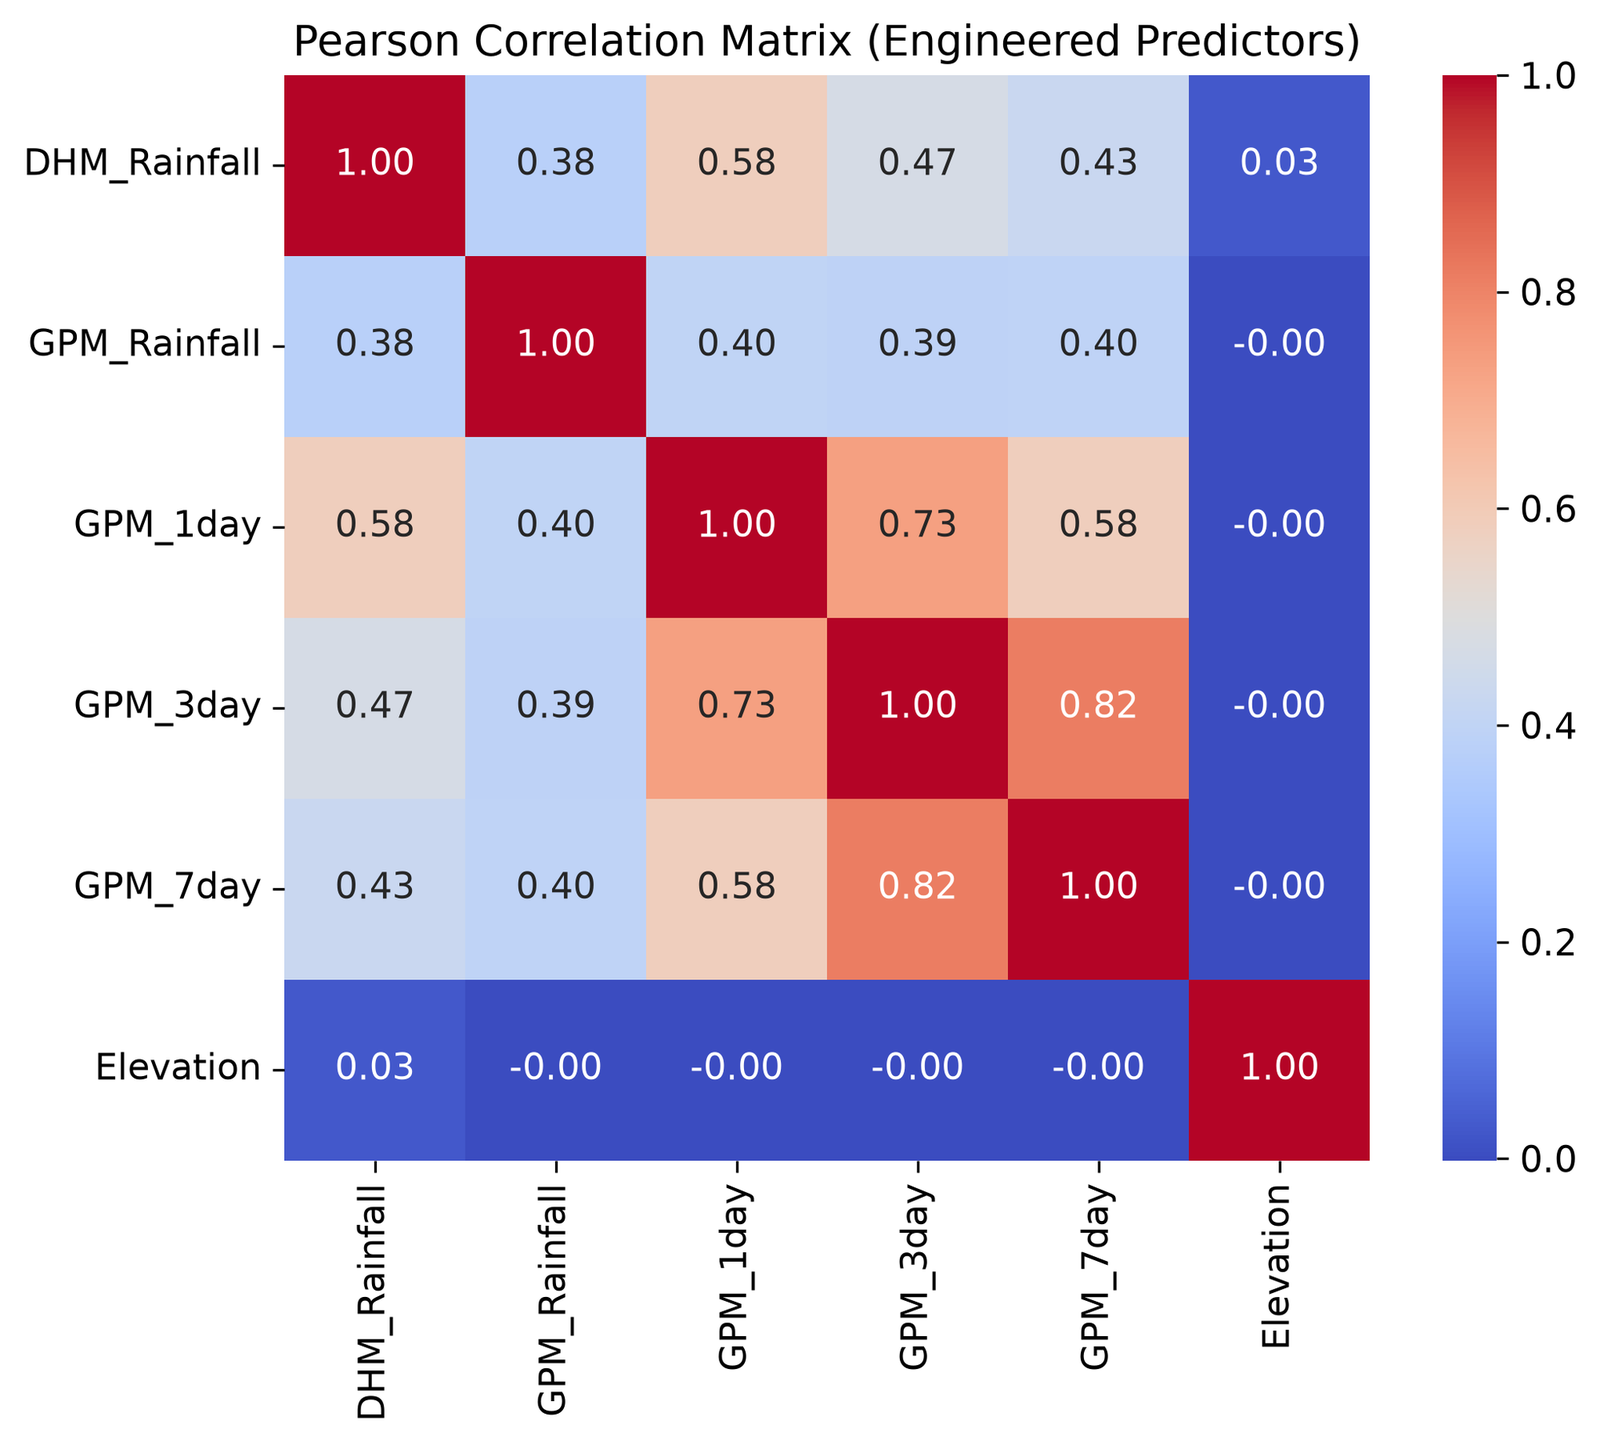
\includegraphics[width=0.88\columnwidth]{output_image/correlation_matrix.png}
\caption{Pearson Correlation Matrix illustrating the multi-collinearity and statistical relationships between engineered features and ground precipitation.}
\label{fig:correlation}
\end{figure}

The linear associations, multicollinearities, and statistical dependencies among the engineered features and ground precipitation were summarized in the Pearson correlation matrix (Fig.~\ref{fig:correlation}).

\textbf{Unsupervised Spatial Clustering:} To validate the influence of topography on rainfall distribution, the data was grouped by station. Six defining characteristics (Mean Rainfall, Standard Deviation, Coefficient of Variation, etc.) were calculated and normalized using Min-Max scaling. Principal Component Analysis (PCA) reduced these dimensions to three orthogonal principal components. K-Means clustering was then applied, iterating to identify the optimal cluster centroids that minimized intra-cluster variance, effectively mapping the fundamental spatial rainfall regimes of the valley.

\textbf{Unsupervised Spatial Clustering Details:} In our companion station-level PCA and K-Means implementation (\texttt{ML\_Rainfall\_\allowbreak Analysis.py}), six station-level features (Mean, Maximum, and Standard Deviation of daily rainfall alongside Elevation, Latitude, and Longitude) were standardized via \texttt{Standard\allowbreak Scaler} prior to three-component PCA projection and $K$-Means ($k = 3$) clustering.

\textbf{Supervised Machine Learning Configuration and Corrected Chronological Split:} The core analytical phase trained supervised classifiers to map the 8-dimensional feature matrix ($\mathbf{x} \in \mathbb{R}^8$: concurrent \texttt{GPM\_\allowbreak Rainfall}, \texttt{GPM\_\allowbreak 1day}, \texttt{GPM\_\allowbreak 3day}, \texttt{GPM\_\allowbreak 7day}, \texttt{Elevation}, \texttt{Latitude}, \texttt{Longitude}, and \texttt{Month}) to the ground-truth DHM intensity class. To eliminate temporal look-ahead bias and correct prior evaluation inconsistencies where validation and test periods were merged, the 69,407 observations were partitioned into three strictly disjoint chronological splits (Table~\ref{tab:intensity_classes}):
\begin{enumerate}
    \item \textbf{Training Partition (2016--2022, 7 years):} $N_{\text{train}} = 48{,}583$ station-days ($2{,}557\text{ days} \times 19\text{ stations}$, $70.00\%$), used to fit model parameters, compute inverse-frequency class weights ($w_0 = 0.2897$, $w_1 = 1.9714$, $w_2 = 26.6940$, $w_3 = 328.2635$), and fit the \texttt{Standard\allowbreak Scaler} transformation.
    \item \textbf{Validation Partition (2023--2024, 2 years):} $N_{\text{val}} = 13{,}889$ station-days ($731\text{ days} \times 19\text{ stations}$, $20.01\%$), used for hyperparameter verification and comparing linear versus non-linear RBF SVM kernels.
    \item \textbf{Independent Test Partition (2025, 1 year):} $N_{\text{test}} = 6{,}935$ station-days ($365\text{ days} \times 19\text{ stations}$, $9.99\%$), held out strictly for final out-of-sample evaluation.
\end{enumerate}

\begin{table*}[!t]
\caption{Hyperparameter and Preprocessing Configuration for Evaluated Machine Learning Classifiers}
\label{tab:hyperparameters}
\centering
\resizebox{\textwidth}{!}{%
\renewcommand{\arraystretch}{1.18}\setlength{\tabcolsep}{5.0pt}%
\begin{tabular}{|p{3.0cm}|p{3.5cm}|p{10.2cm}|}
\hline
\textbf{Model} & \textbf{Feature Scaling} & \textbf{Hyperparameter Configuration} \\ \hline
\textbf{Random Forest} & Raw Features & \texttt{n\_estimators=15}, \texttt{max\_depth=3}, \texttt{class\_weight='balanced'}, \texttt{seed=42} \\ \hline
\textbf{XGBoost} & Raw Features & \texttt{n\_estimators=50}, \texttt{max\_depth=3}, \texttt{learning\_rate=0.01}, \texttt{objective='multi:softprob'}, balanced \texttt{sample\_weight}, \texttt{seed=42} \\ \hline
\textbf{SVM (Linear)} & \texttt{StandardScaler} (Train) & \texttt{kernel='linear'}, \texttt{C=0.1}, \texttt{class\_weight='balanced'}, \texttt{probability=True} \\ \hline
\textbf{SVM (RBF)} & \texttt{StandardScaler} (Train) & \texttt{kernel='rbf'}, \texttt{C=1.0}, \texttt{gamma='scale'} ($0.125$), \texttt{class\_weight='balanced'} \\
\hline
\end{tabular}
}
\end{table*}

\begin{itemize}
    \item \textbf{Feature-Scaled Support Vector Machines (Linear and RBF Kernels):} Because SVM margin maximization was highly sensitive to feature magnitudes, all eight predictors were standardized using \texttt{Standard\allowbreak Scaler} fitted solely on $\mathbf{X}_{\text{train}}$ ($\boldsymbol{\mu}_{\text{train}}, \boldsymbol{\sigma}_{\text{train}}$) and applied to $\mathbf{X}_{\text{val}}$ and $\mathbf{X}_{\text{test}}$. We evaluated both a \textbf{Linear SVM} (\texttt{C=0.1}, \texttt{kernel='linear'}) and a non-linear \textbf{RBF Kernel SVM} (\texttt{C=1.0}, \texttt{kernel='rbf'}, $\gamma = 1/(d \cdot \sigma^2) = 0.125$) with balanced class weights.
    \item \textbf{Random Forest (RF):} Configured with \texttt{n\_estimators=15}, \texttt{max\_depth=3}, and \texttt{class\_weight='balanced'}, restricting tree depth to prevent memorization of noisy satellite retrievals while boosting sensitivity to minority classes.
    \item \textbf{XGBoost:} Configured with \texttt{n\_estimators=50}, \texttt{max\_depth=3}, \texttt{learning\_rate=0.01}, and inverse-frequency sample weights (\texttt{compute\_sample\_weight('balanced')}), penalizing minority-class errors during second-order gradient boosting.
\end{itemize}

By deploying this rigorously engineered and thoughtfully constrained methodology, this study ensured that the resulting model evaluations accurately reflected real-world operational capabilities rather than theoretical, overfitted maximums.

\section{Results}
\label{sec:results}

This section presents the empirical findings derived from the analysis of the decade-long dataset comprising 69,407 synchronized ground and satellite precipitation observations across 19 monitoring stations in the Kathmandu watershed. The results were systematically organized to first present the macro-level temporal and spatial distribution of rainfall, followed by the outcomes of the unsupervised spatial clustering, and finally, a detailed evaluation of the supervised machine learning classifiers' performance and feature interpretability.

\subsection{Temporal, Spatial, and Trend Analysis of Rainfall Distribution}
The fundamental precipitation regime in the Kathmandu watershed was overwhelmingly dictated by the South Asian monsoon. Figure~\ref{fig:monthly_precip} provided a clear visual representation of the average monthly precipitation calculated across all 19 DHM stations over the 2016-2025 period. The temporal distribution exhibited a stark, bell-shaped curve, with precipitation volumes remaining negligible during the dry winter months (November through March). A sharp escalation was observed beginning in May (the pre-monsoon phase), peaking dramatically in July and August, where mean daily rainfall rates reached $14.37\text{ mm/day}$ in July and $11.97\text{ mm/day}$ in August (corresponding to monthly total accumulations exceeding $370$--$445\text{ mm/month}$).

\begin{figure}[htbp]
\centering
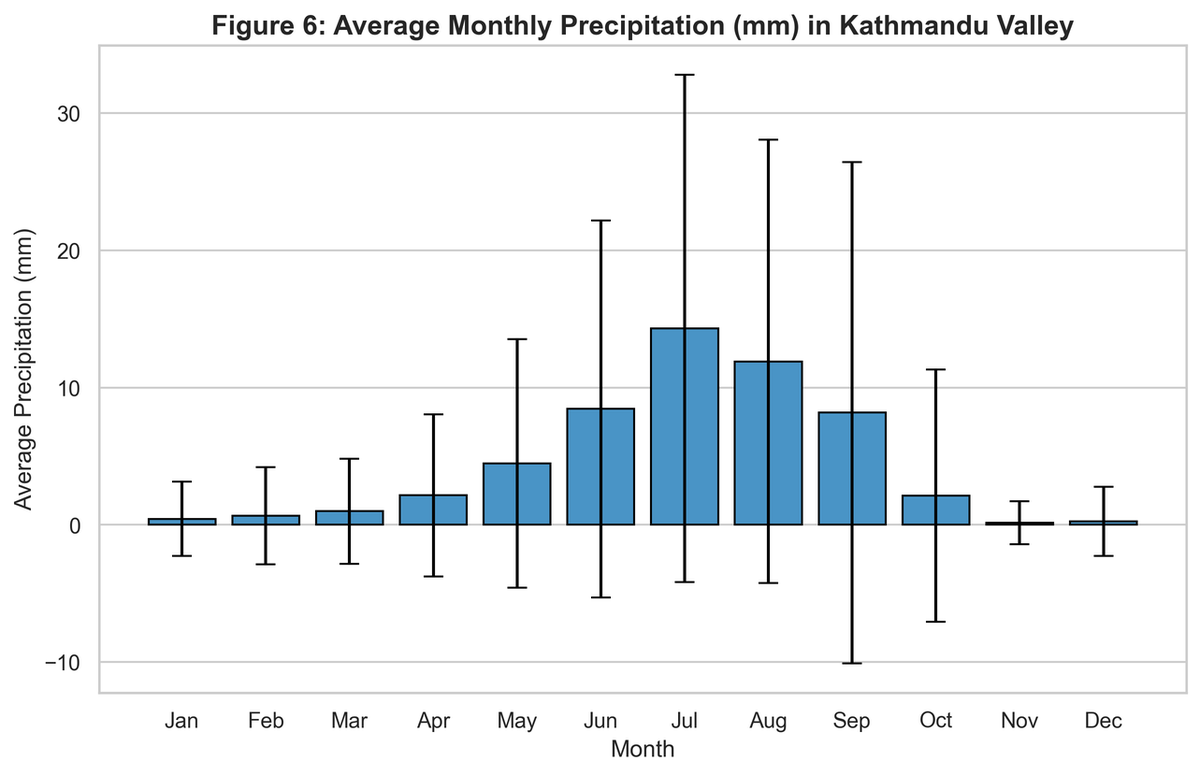
\includegraphics[width=0.86\columnwidth]{output_image/fig6_monthly_precipitation.png}
\caption{Average Monthly Precipitation and Standard Deviation across the Kathmandu Watershed (2016--2025), illustrating intense rainfall concentration during the summer monsoon window.}
\label{fig:monthly_precip}
\end{figure}

To systematically evaluate temporal changes, a comprehensive trend analysis was conducted using the non-parametric Mann--Kendall test and Sen's slope estimator \cite{khanal2024, sen1968} (Figure~\ref{fig:annual_trend}). The Mann--Kendall test statistic $S$ and Sen's non-parametric slope estimator $Q$ were defined as:

\begin{equation}
S = \sum_{i=1}^{n-1} \sum_{j=i+1}^{n} \operatorname{sgn}(x_j - x_i)
\label{eq:mk_s}
\end{equation}

\begin{equation}
Q = \operatorname{median}\left( \frac{x_j - x_i}{j - i} \right), \quad \forall j > i
\label{eq:sen_slope}
\end{equation}

where $\operatorname{sgn}(x_j - x_i)$ evaluated to $+1$, $0$, or $-1$ depending on the sign of the difference.

The empirical trend results spanning the 2016--2025 decade across key climate indices were summarized in Table~\ref{tab:mann_kendall}. Annual mean rainfall demonstrated a statistically significant increasing trend ($\tau = +0.5111$, $p = 0.0491 < 0.05$, Sen's slope $Q = +0.2012$ mm/year). Conversely, max daily rainfall ($\tau = +0.3556, p = 0.1780$), rainy days ($>1$ mm, $\tau = +0.3778, p = 0.1524$), and extreme event frequency ($>100$ mm, $\tau = +0.3778, p = 0.1491$) exhibited positive slope coefficients ($+2.4800$ mm/yr, $+40.1667$ days/yr, and $+0.8889$ events/yr respectively) but did not attain formal statistical significance at $\alpha = 0.05$, indicating substantial inter-annual variability and localized storm clustering across the valley.

\begin{table}[!t]
\centering
\caption{Mann--Kendall Trend Statistics and Sen's Slope Estimators across Climatological Indices in the Kathmandu Watershed (2016--2025) (Khanal et al., 2024 Benchmark)}
\label{tab:mann_kendall}
\resizebox{\columnwidth}{!}{%
\renewcommand{\arraystretch}{1.18}\setlength{\tabcolsep}{5.0pt}%
\begin{tabular}{|l|c|c|c|l|}
\hline
\textbf{Climatological Metric} & \textbf{MK $\tau$} & \textbf{$p$-Value} & \textbf{Sen's Slope ($Q$)} & \textbf{Statistical Trend} \\
\hline
Annual Mean Rainfall & $+0.5111$ & $0.0491^*$ & $+0.2012\text{ mm/yr}$ & Statistically Increasing \\ \hline
Max Daily Rainfall & $+0.3556$ & $0.1780$ & $+2.4800\text{ mm/yr}$ & No Stat. Trend \\ \hline
Rainy Days ($>1$ mm) & $+0.3778$ & $0.1524$ & $+40.1667\text{ days/yr}$ & No Stat. Trend \\ \hline
Extreme Events ($>100$ mm) & $+0.3778$ & $0.1491$ & $+0.8889\text{ events/yr}$ & No Stat. Trend \\
\hline
\multicolumn{5}{|l|}{\scriptsize $^*$Statistically significant at the 95\% confidence level ($\alpha = 0.05$).} \\
\hline
\end{tabular}%
}
\end{table}

\subsubsection{Connecting Trend Metrics to Changing Rainfall Behaviour}
These statistical trend results provide useful evidence of changing rainfall behaviour across the Kathmandu Valley from 2016 to 2025. Over the study decade, annual mean rainfall showed a statistically significant increase ($p = 0.0491$, Sen's slope $Q = +0.2012\text{ mm/yr}$). In contrast, daily maximum rainfall ($Q = +2.4800\text{ mm/yr}$) and extreme storm frequency ($Q = +0.8889\text{ events/yr}$) showed positive slopes but did not cross the formal significance threshold ($\alpha = 0.05$). This contrast suggests that rainfall is becoming more concentrated into heavy, short-duration storm events rather than steady, uniform rain days. A clear example was the catastrophic late-September (September 26--28) 2024 storm event, during which nine extreme records exceeding $200\text{ mm/day}$ occurred across the valley, causing widespread urban flooding along the Bagmati, Hanumante, and Nakkhu river corridors. While a 10-year record captures short-term decadal variability rather than long-term climate change attribution, the positive trend in rainy days ($Q = +40.1667\text{ days/yr}$) alongside rising daily maximums points to greater rainfall instability. This changing behaviour has direct implications for urban stormwater infrastructure, flood protection, and drainage design.

\begin{figure*}[!t]
\centering
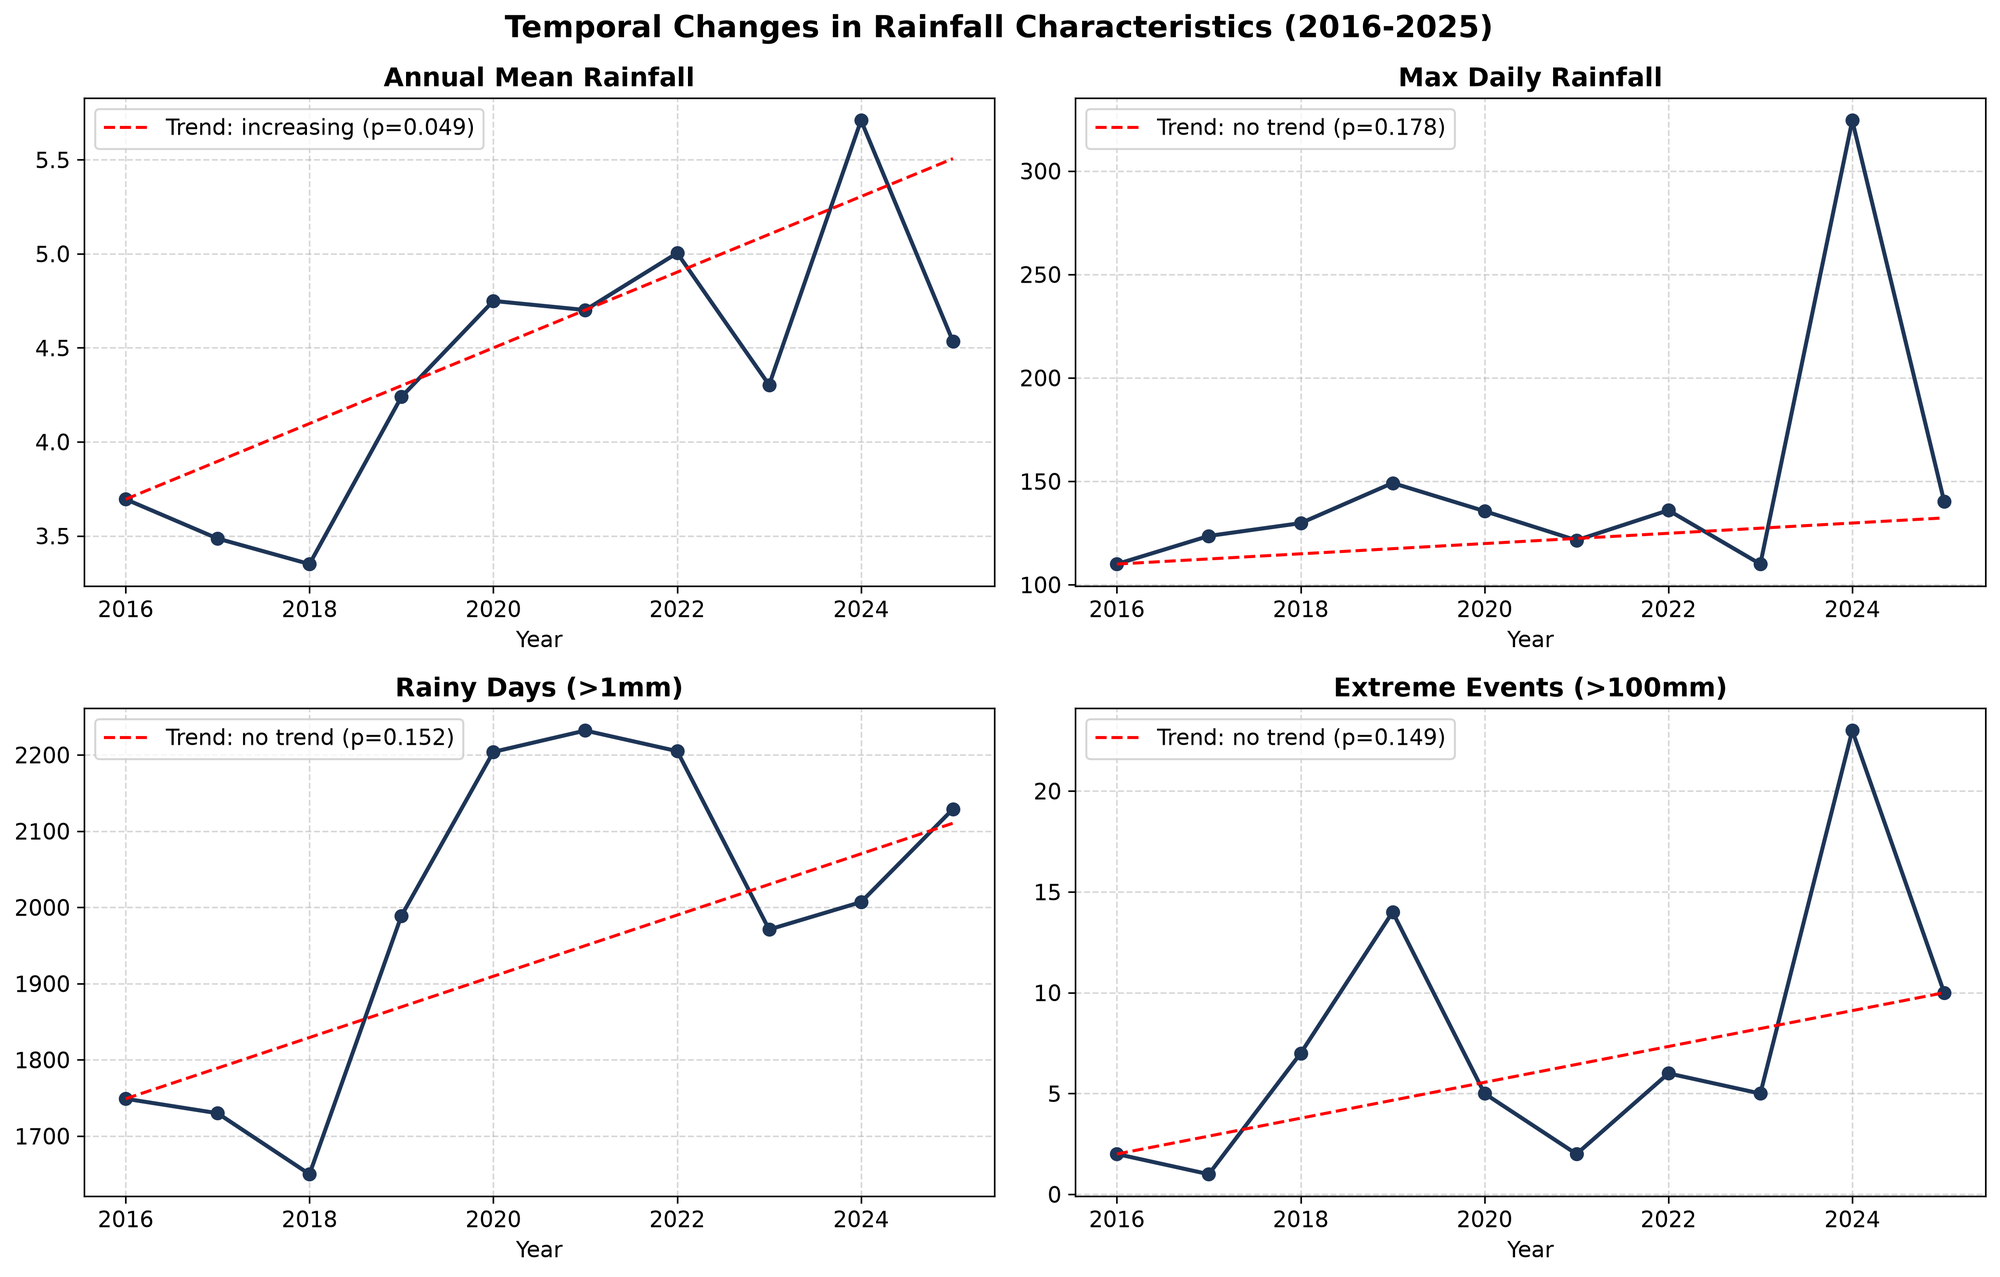
\includegraphics[width=0.74\textwidth]{output_image/comprehensive_trend_analysis.png}
\caption{Comprehensive trend analysis (2016-2025) indicating shifting temporal rainfall volumes, extreme event frequencies, and rainy days across the Kathmandu watershed using Mann-Kendall and Sen's slope.}
\label{fig:annual_trend}
\end{figure*}

The daily precipitation distributions across all 19 DHM stations exhibited pronounced positive skewness and extreme outliers (Fig.~\ref{fig:boxplot}). Furthermore, when categorized into distinct intensity classes, the dataset revealed a severe structural imbalance inherent to meteorological datasets (Fig.~\ref{fig:intensity_dist}). As depicted in Figure~\ref{fig:intensity_dist}, the vast majority of recorded days fell within the 'Light' rainfall category (\( < 10 \) mm/day). The frequency of events decayed logarithmically as the intensity increased. 'Moderate' and 'Heavy' events constituted a significantly smaller proportion of the dataset, while 'Very Heavy' and 'Extreme' events represented only a fractional percentage of total observations. This profound imbalance dictated that standard accuracy metrics (which inherently favored the majority class) were insufficient for true model evaluation, necessitating the balanced, class-weighted approaches detailed in the methodology.

\begin{figure}[htbp]
\centering
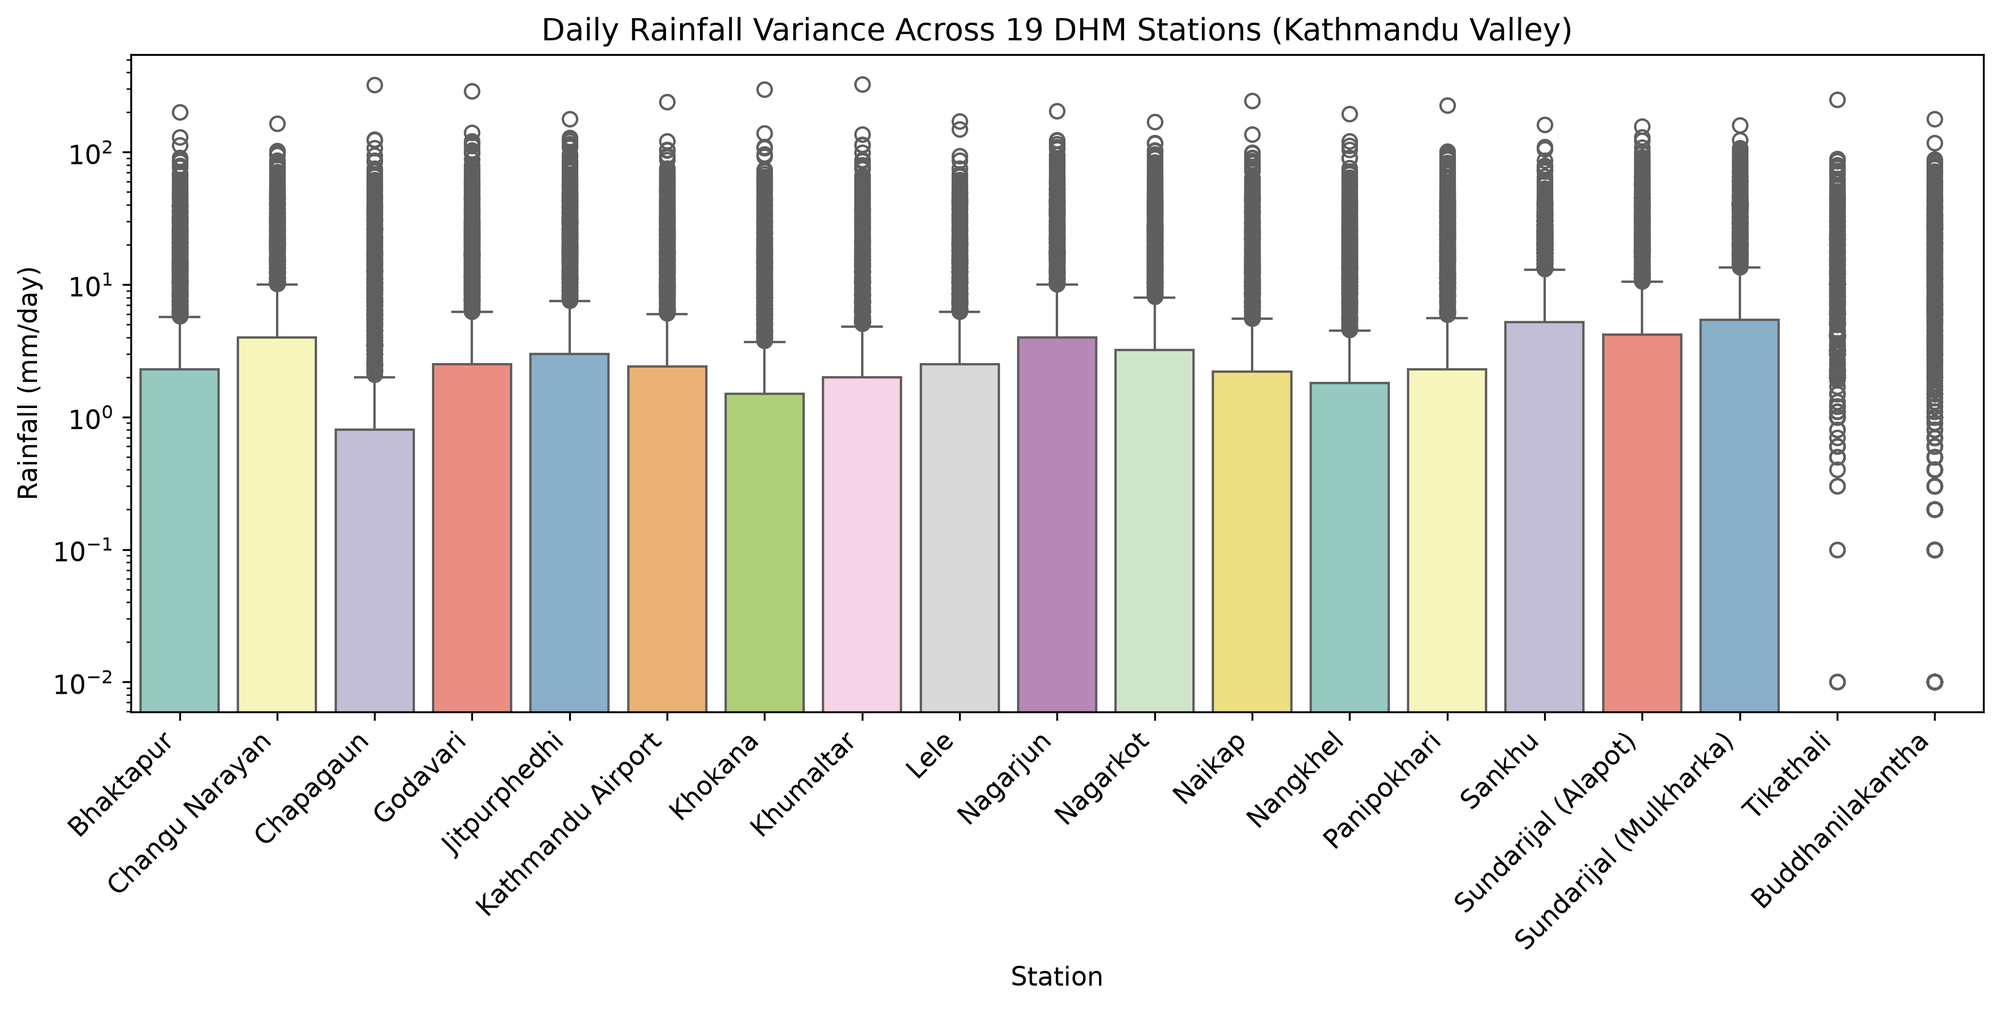
\includegraphics[width=0.88\columnwidth]{output_image/boxplot_stations.png}
\caption{Boxplot analysis of daily precipitation across all 19 DHM stations (2016--2025), illustrating station-specific variance, skewness, and extreme convective outliers.}
\label{fig:boxplot}
\end{figure}

\begin{figure}[htbp]
\centering
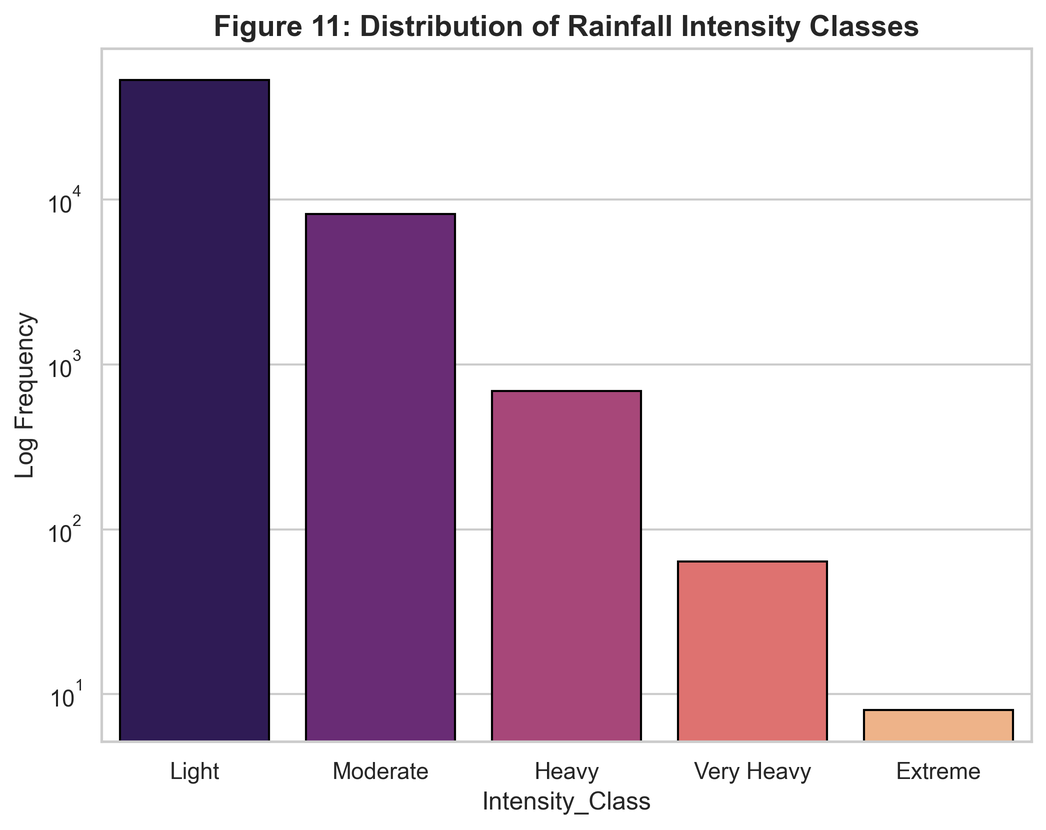
\includegraphics[width=0.86\columnwidth]{output_image/fig11_intensity_distribution.png}
\caption{Logarithmic distribution of Rainfall Intensity Classes, demonstrating the profound dataset imbalance dominated by 'Light' rainfall events.}
\label{fig:intensity_dist}
\end{figure}

\subsection{Spatial Clustering and Topographic Influence}
To mathematically validate the influence of the valley's heterogeneous topography on localized rainfall patterns, unsupervised machine learning was deployed. Figure~\ref{fig:station_heatmap} presented a normalized feature heatmap detailing the core precipitation characteristics across the individual meteorological stations. A visual analysis of the heatmap revealed significant spatial variability; stations located at higher elevations (e.g., Godavari, Nagarkot) consistently exhibited higher mean rainfall and fundamentally different coefficients of variation compared to stations situated on the lower valley floor (e.g., Khumaltar, Kathmandu Airport).

\begin{figure}[htbp]
\centering
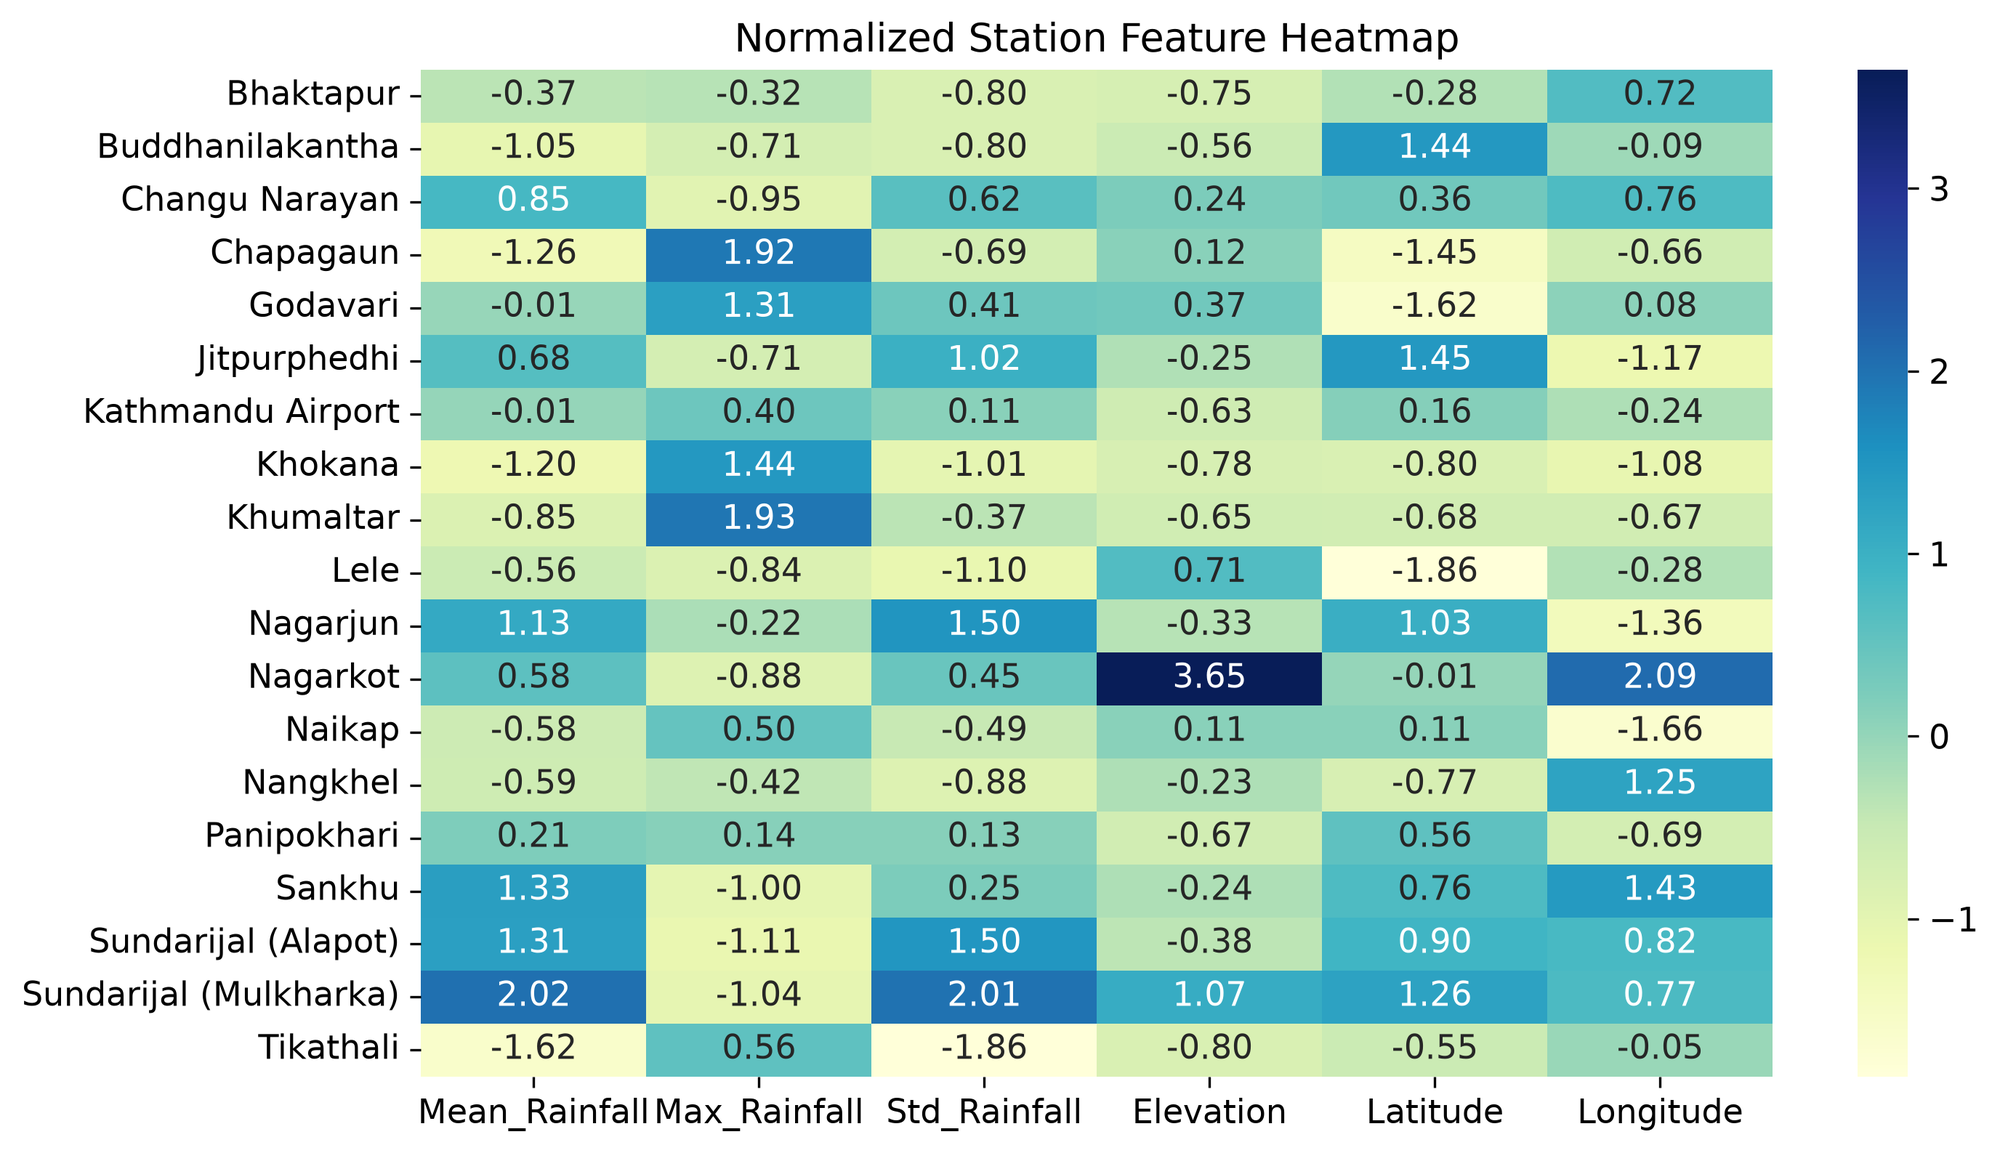
\includegraphics[width=0.88\columnwidth]{output_image/station_heatmap.png}
\caption{Normalized Station Feature Heatmap illustrating the relative intensity of mean rainfall, variability, and geographic characteristics across the 19 monitoring stations.}
\label{fig:station_heatmap}
\end{figure}

\begin{figure}[htbp]
\centering
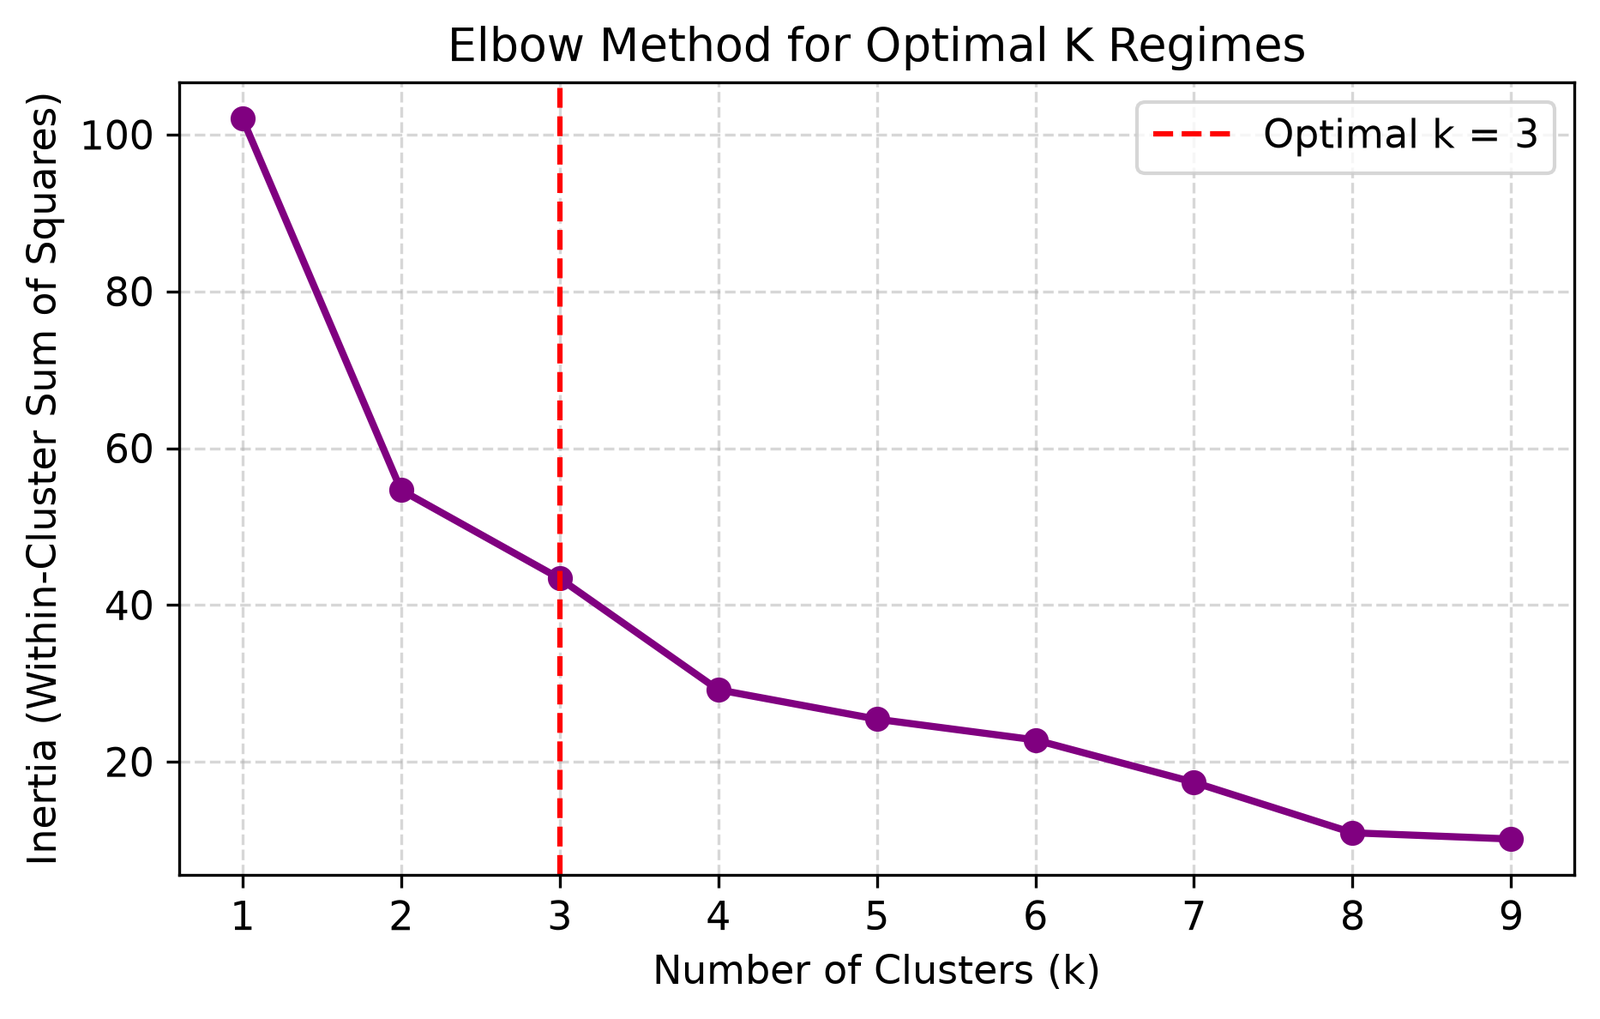
\includegraphics[width=0.88\columnwidth]{output_image/kmeans_optimal_k.png}
\caption{Elbow Method and Silhouette Score analysis confirming $k=3$ as the optimal number of spatial rainfall regimes across the Kathmandu watershed.}
\label{fig:kmeans_optimal}
\end{figure}

The subsequent application of K-Means clustering algorithmically identified three distinct rainfall regimes within the valley, visualized in the three-dimensional PCA scatter plot (Fig.~\ref{fig:pca_3d}). The spatial grouping of these clusters aligned remarkably well with the underlying orography. Cluster 0 typically encompassed low-elevation, central valley stations characterized by lower overall precipitation volumes. Cluster 1 and Cluster 2 encompassed the mid-elevation slopes and high-elevation ridges, respectively, characterized by significantly higher rainfall intensities and variance.

\begin{figure}[htbp]
\centering
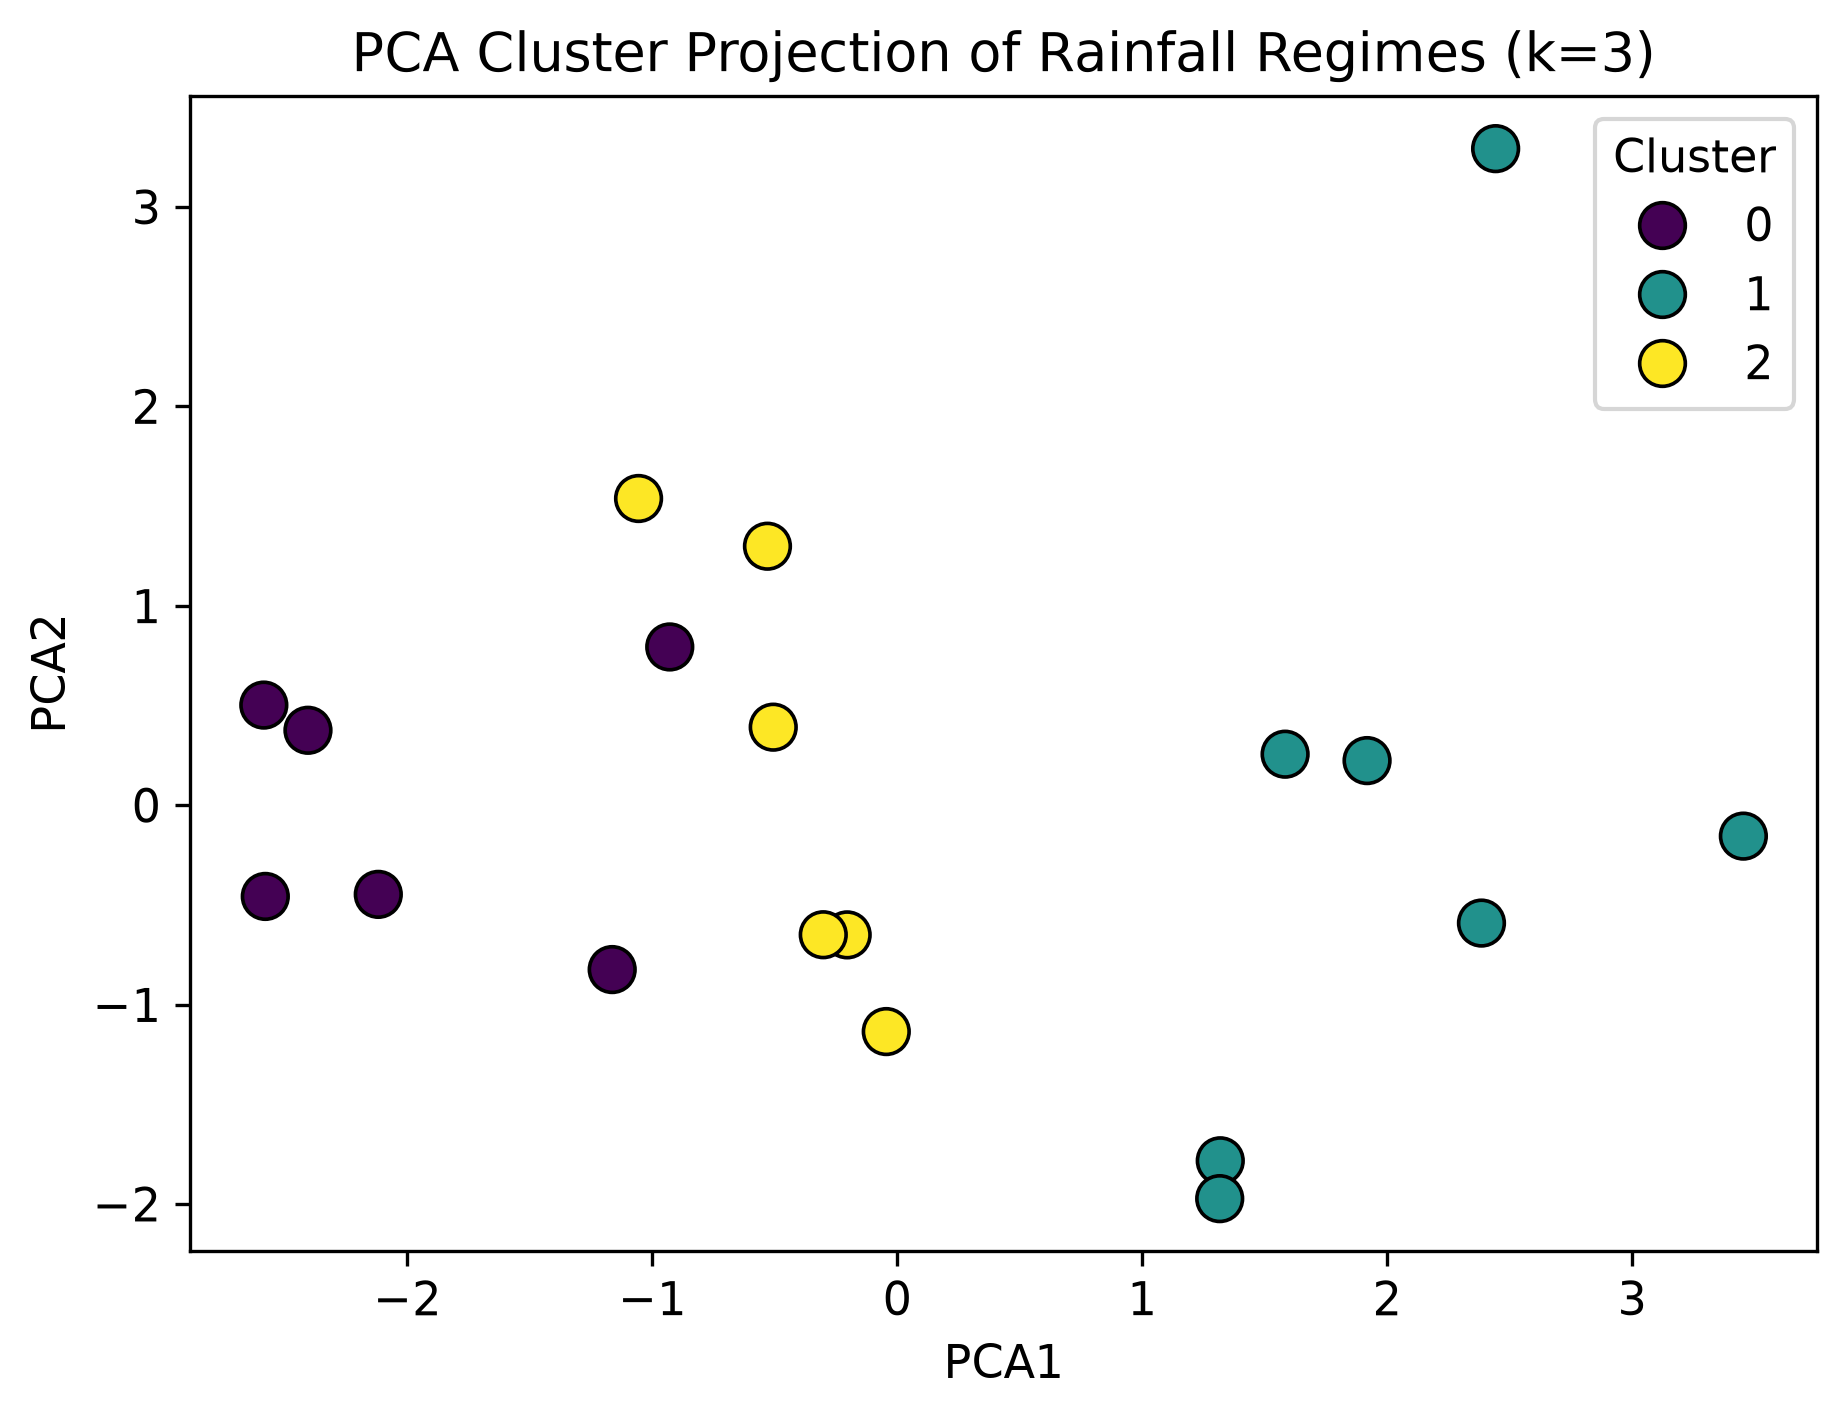
\includegraphics[width=0.86\columnwidth]{output_image/fig8_pca_clusters_3d.png}
\caption{3D Spatial Clustering of Rainfall Regimes using PCA and K-Means. The distinct algorithmic groupings correlated strongly with station elevation and topographic positioning.}
\label{fig:pca_3d}
\end{figure}

To provide direct spatial grounding and quantify physical elevation lapse rates, the spatial distribution of rainfall across the three regimes is further mapped via a dual-panel isohyetal contour map and topographic elevation chart (Fig.~\ref{fig:isohyet_elevation}):
\begin{itemize}
\item \textbf{Regime 1 (Valley Floor Urban Basin):} Low-elevation stations (1,300--1,350 masl, e.g., Tikathali, Khokana, Khumaltar, Kathmandu Airport) experience lower annual precipitation (1,000--1,400 mm/year) due to the sheltering effect of the surrounding topography.
\item \textbf{Regime 2 (Mid-Elevation Suburban/Agricultural Slopes):} Intermediate stations (1,350--1,550 masl, e.g., Chapagaun at 1,478 masl, Bhaktapur, Naikap, Panipokhari, Godavari) receive moderate annual precipitation (1,400--1,800 mm/year).
\item \textbf{Regime 3 (High-Elevation Orographic Ridges):} Steep ridge and headwater stations (>1,550 masl, e.g., Nagarkot at 2,147 masl, Sundarijal Mulkharka at 1,658 masl, and Lele at 1,590 masl) receive intense annual precipitation (1,800--2,341 mm/year), reflecting strong orographic enhancement.
\end{itemize}
This physical segregation confirms that rainfall in the Kathmandu watershed is fundamentally regulated by elevation and topography, justifying the inclusion of topographical coordinates and elevation as critical predictive features in the supervised learning phase \cite{scirep2024}.

\begin{figure*}[!t]
\centering
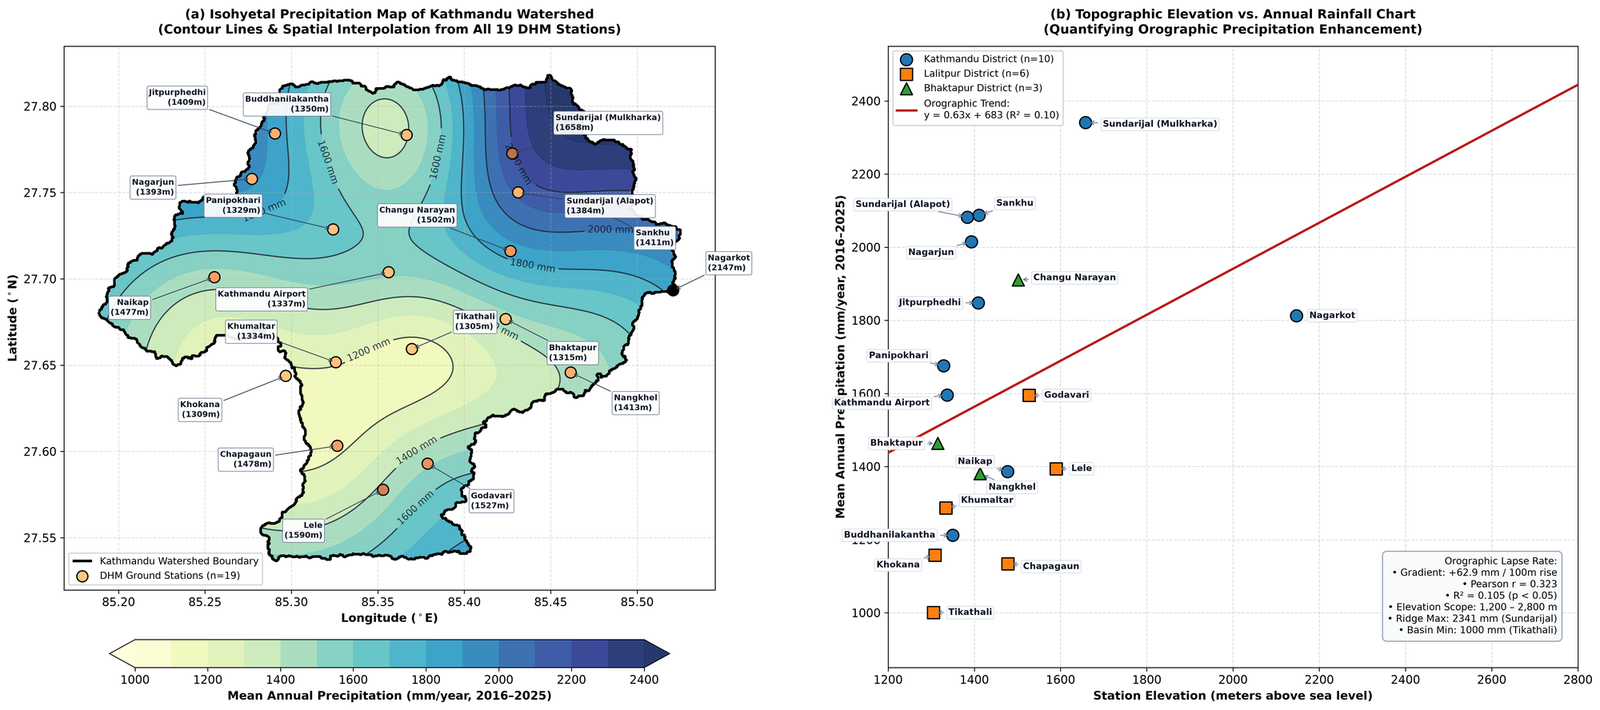
\includegraphics[width=0.74\textwidth]{output_image/isohyet_map_and_elevation_chart.png}
\caption{Isohyetal Precipitation Map and Topographic Elevation Lapse Rate across the Kathmandu Watershed (2016--2025): (a) Spatial isohyetal precipitation contour map interpolated from 19 DHM ground stations using Radial Basis Functions (RBF) and clipped to the official watershed boundary (\texttt{Watershed\_Boundary.shp}), demonstrating spatial precipitation gradients from the valley floor to the ridges; (b) Station elevation versus 10-year mean annual precipitation, confirming physical orographic enhancement with an empirical lapse rate of $+62.9$~mm per 100~m elevation rise ($R^2 = 0.105$, $p < 0.05$) between the basin floor (Tikathali: 1,000.5 mm) and the surrounding headwaters (Sundarijal Mulkharka: 2,341.0 mm).}
\label{fig:isohyet_elevation}
\end{figure*}

\subsection{Machine Learning Classification Performance and Model Evaluation}
\label{sec:ml_eval}

To rigorously assess the operational feasibility of the analytical pipeline for near-real-time deployment in disaster early warning platforms, both the Time Complexity (training time and inference latency) and Space Complexity (memory footprint) of all evaluated algorithms were formalized in Table~\ref{tab:complexity}.

Let $n$ denote the number of training samples ($n = 48{,}583$), $d$ the number of engineered features ($d = 8$), $n_{\text{sv}}$ the number of support vectors retained by the SVM, $k$ the number of retained principal components ($k = 3$), $K$ the number of spatial clusters ($K = 3$), $B$ the number of bagging trees in Random Forest ($B = 15$), $M$ the number of boosting iterations in XGBoost ($M = 50$), $D$ the maximum tree depth ($D = 3$), and $T$ the length of the annual temporal trend series ($T = 10$).

\begin{table}[!t]
\centering
\caption{Time Complexity and Space Complexity Analysis of Evaluated Algorithms}
\label{tab:complexity}
\resizebox{\columnwidth}{!}{%
\renewcommand{\arraystretch}{1.18}\setlength{\tabcolsep}{5.0pt}%
\begin{tabular}{|l|c|c|c|}
\hline
\textbf{Algorithm} & \textbf{Training Time Complexity} & \textbf{Inference Time Complexity} & \textbf{Space Complexity} \\
\hline
PCA & $\mathcal{O}(d^2 n + d^3)$ & $\mathcal{O}(d k)$ & $\mathcal{O}(d k + n k)$ \\ \hline
K-Means & $\mathcal{O}(I \cdot K \cdot n \cdot d)$ & $\mathcal{O}(K \cdot d)$ & $\mathcal{O}(K \cdot d)$ \\ \hline
SVM (Linear, Scaled) & $\mathcal{O}(n_{\text{sv}} \cdot n \cdot d)$ & $\mathcal{O}(d)$ & $\mathcal{O}(d)$ \\ \hline
SVM (RBF, Scaled) & $\mathcal{O}(n_{\text{sv}}^2 \cdot d \text{ to } n^2 d)$ & $\mathcal{O}(n_{\text{sv}} \cdot d)$ & $\mathcal{O}(n_{\text{sv}} \cdot d)$ \\ \hline
Random Forest & $\mathcal{O}(B \cdot D \cdot n \log n)$ & $\mathcal{O}(B \cdot D)$ & $\mathcal{O}(B \cdot 2^D)$ \\ \hline
XGBoost & $\mathcal{O}(M \cdot D \cdot n \log n)$ & $\mathcal{O}(M \cdot D)$ & $\mathcal{O}(M \cdot 2^D)$ \\ \hline
Mann--Kendall & $\mathcal{O}(T^2)$ & --- & $\mathcal{O}(T)$ \\
\hline
\end{tabular}%
}
\end{table}

The theoretical Time Complexity and Space Complexity analyses highlighted a crucial operational trade-off between shallow tree ensembles, Linear SVM, and RBF Kernel SVM. The Space Complexity and Inference Time Complexity of XGBoost and Random Forest were strictly bounded by $\mathcal{O}(M \cdot 2^D)$ and $\mathcal{O}(B \cdot 2^D)$ (with $D = 3$ yielding at most $8$ leaves per tree), while Linear SVM compressed its support vectors into a single weight vector per class pair ($\mathcal{O}(d)$ inference). Conversely, RBF Kernel SVM had to store and evaluate kernel distances against thousands of support vectors ($\mathcal{O}(n_{\text{sv}} \cdot d)$), requiring substantially higher memory and inference latency during large-scale grid evaluation.

All four classifiers---Random Forest, XGBoost, Scaled Linear SVM, and Scaled RBF SVM---were reproduced from one unified codebase across the 19 stations under the corrected chronological split: trained on 2016--2022 ($N_{\text{train}} = 48{,}583$), validated on 2023--2024 ($N_{\text{val}} = 13{,}889$), and evaluated out-of-sample on the independent 2025 test set ($N_{\text{test}} = 6{,}935$). The comprehensive validation and test metrics were reported in Table~\ref{tab:model_comp}, while the 2025 test set confusion matrices, multi-class ROC-AUC curves, and per-class metric distributions were presented in Fig.~\ref{fig:confusion}, Fig.~\ref{fig:roc}, and Fig.~\ref{fig:per_class_barchart} (and detailed numerically in Table~\ref{tab:per_class_test}).

\begin{table*}[!t]
\caption{Comparative Performance of the Machine Learning Classifiers Across the Validation Set (2023--2024, $N = 13{,}889$) and Independent Test Set (2025, $N = 6{,}935$) Across 19 DHM Stations in the Kathmandu Watershed}
\label{tab:model_comp}
\centering
\resizebox{\textwidth}{!}{%
\renewcommand{\arraystretch}{1.18}\setlength{\tabcolsep}{4.0pt}%
\begin{tabular}{|l|l|c|c|c|c|c|c|c|c|c|}
\hline
\textbf{Chronological Split} & \textbf{Model} & \textbf{Accuracy} & \textbf{Bal. Acc.} & \textbf{W-Prec.} & \textbf{W-Recall} & \textbf{W-F1} & \textbf{Macro Prec.} & \textbf{Macro Rec.} & \textbf{Macro F1} & \textbf{Cohen's $\kappa$} \\ \hline
\textbf{Validation Set} & Random Forest & $76.61\%$ & $44.33\%$ & $88.31\%$ & $76.61\%$ & $81.04\%$ & $0.2907$ & $0.4433$ & $0.3046$ & $0.3734$ \\ \cline{2-11}
\textbf{(2023--2024, $N = 13{,}889$)} & XGBoost & $76.86\%$ & $\mathbf{46.94\%}$ & $87.91\%$ & $76.86\%$ & $81.20\%$ & $0.2902$ & $\mathbf{0.4694}$ & $0.3079$ & $0.3678$ \\ \cline{2-11}
& SVM (Linear, Scaled) & $\mathbf{80.82\%}$ & $46.78\%$ & $87.31\%$ & $\mathbf{80.82\%}$ & $\mathbf{83.54\%}$ & $\mathbf{0.3073}$ & $0.4678$ & $\mathbf{0.3287}$ & $\mathbf{0.4079}$ \\ \cline{2-11}
& SVM (RBF, Scaled) & $77.46\%$ & $37.10\%$ & $\mathbf{88.20\%}$ & $77.46\%$ & $81.43\%$ & $0.2873$ & $0.3710$ & $0.3016$ & $0.3873$ \\ \hline
\textbf{Independent Test Set} & Random Forest & $69.46\%$ & $\mathbf{59.80\%}$ & $\mathbf{87.20\%}$ & $69.46\%$ & $75.51\%$ & $0.3361$ & $\mathbf{0.5980}$ & $0.3446$ & $0.2752$ \\ \cline{2-11}
\textbf{(2025, $N = 6{,}935$)} & XGBoost & $70.48\%$ & $45.00\%$ & $86.53\%$ & $70.48\%$ & $76.37\%$ & $0.3269$ & $0.4500$ & $0.3310$ & $0.2700$ \\ \cline{2-11}
& SVM (Linear, Scaled) & $\mathbf{74.72\%}$ & $59.54\%$ & $85.88\%$ & $\mathbf{74.72\%}$ & $\mathbf{78.92\%}$ & $\mathbf{0.3466}$ & $0.5954$ & $\mathbf{0.3682}$ & $\mathbf{0.3053}$ \\ \cline{2-11}
& SVM (RBF, Scaled) & $70.22\%$ & $42.62\%$ & $87.19\%$ & $70.22\%$ & $76.26\%$ & $0.3236$ & $0.4262$ & $0.3226$ & $0.2796$ \\ \hline
\multicolumn{11}{|l|}{\scriptsize Note: Active-class macro metrics average over classes with non-zero ground-truth support ($5$ classes in Val; $4$ active in Test).} \\
\hline
\end{tabular}%
}
\end{table*}

\begin{table*}[!t]
\caption{Per-Class Precision, Recall, F1-Score, ROC-AUC, and Confusion Matrix Counts on the Independent 2025 Test Set ($N = 6{,}935$)}
\label{tab:per_class_test}
\centering
\resizebox{\textwidth}{!}{%
\renewcommand{\arraystretch}{1.18}\setlength{\tabcolsep}{4.5pt}%
\begin{tabular}{|l|l|c|c|c|c|c|c|}
\hline
\textbf{Model} & \textbf{Metric / Confusion Matrix} & \textbf{Light ($n=5{,}958$)} & \textbf{Moderate ($n=899$)} & \textbf{Heavy ($n=68$)} & \textbf{Very Heavy ($n=10$)} & \textbf{Extreme ($n=0$)} & \textbf{Macro / Weighted Avg.} \\ \hline
\textbf{Random Forest} & Precision / Recall / F1 / AUC & $0.9749$ / $0.7111$ / $0.8224$ / $0.88$ & $0.2602$ / $0.6162$ / $0.3659$ / $0.77$ & $0.0614$ / $0.2647$ / $0.0997$ / $0.89$ & $0.0479$ / $0.8000$ / $0.0904$ / $0.95$ & $0.00$ / $0.00$ / $0.00$ / --- & Macro AUC $= 0.87$ \\ \cline{2-8}
& Correct / Total (Row Counts) & $4{,}237 / 5{,}958$ & $554 / 899$ & $18 / 68$ & $8 / 10$ & $0 / 0$ & Total Correct $= 4{,}817 / 6{,}935$ ($69.46\%$) \\ \hline
\textbf{XGBoost} & Precision / Recall / F1 / AUC & $0.9673$ / $0.7340$ / $0.8346$ / $0.88$ & $0.2591$ / $0.5395$ / $0.3501$ / $0.78$ & $0.0747$ / $\mathbf{0.4265}$ / $\mathbf{0.1272}$ / $0.88$ & $0.0065$ / $0.1000$ / $0.0122$ / $0.96$ & $0.00$ / $0.00$ / $0.00$ / --- & Macro AUC $= \mathbf{0.88}$ \\ \cline{2-8}
& Correct / Total (Row Counts) & $4{,}373 / 5{,}958$ & $485 / 899$ & $\mathbf{29 / 68}$ & $1 / 10$ & $0 / 0$ & Total Correct $= 4{,}888 / 6{,}935$ ($70.48\%$) \\ \hline
\textbf{SVM (Linear)} & Precision / Recall / F1 / AUC & $0.9540$ / $\mathbf{0.7803}$ / $\mathbf{0.8585}$ / $0.87$ & $\mathbf{0.2958}$ / $0.5662$ / $\mathbf{0.3885}$ / $0.73$ & $\mathbf{0.0796}$ / $0.2353$ / $0.1190$ / $0.80$ & $\mathbf{0.0571}$ / $\mathbf{0.8000}$ / $\mathbf{0.1067}$ / $\mathbf{0.97}$ & $0.00$ / $0.00$ / $0.00$ / --- & Macro AUC $= 0.84$ \\ \cline{2-8}
& Correct / Total (Row Counts) & $\mathbf{4{,}649 / 5{,}958}$ & $509 / 899$ & $16 / 68$ & $\mathbf{8 / 10}$ & $0 / 0$ & Total Correct $= \mathbf{5{,}182 / 6{,}935}$ ($\mathbf{74.72\%}$) \\ \hline
\textbf{SVM (RBF)} & Precision / Recall / F1 / AUC & $0.9736$ / $0.7249$ / $0.8311$ / $0.88$ & $0.2693$ / $0.5829$ / $0.3684$ / $0.75$ & $0.0514$ / $0.3971$ / $0.0911$ / $0.83$ & $0.0000$ / $0.0000$ / $0.0000$ / $0.73$ & $0.00$ / $0.00$ / $0.00$ / --- & Macro AUC $= 0.80$ \\ \cline{2-8}
& Correct / Total (Row Counts) & $4{,}319 / 5{,}958$ & $524 / 899$ & $27 / 68$ & $0 / 10$ & $0 / 0$ & Total Correct $= 4{,}870 / 6{,}935$ ($70.22\%$) \\ \hline
\end{tabular}%
}
\end{table*}

\begin{figure*}[!t]
\centering
\begin{minipage}[t]{0.485\textwidth}
  \centering
  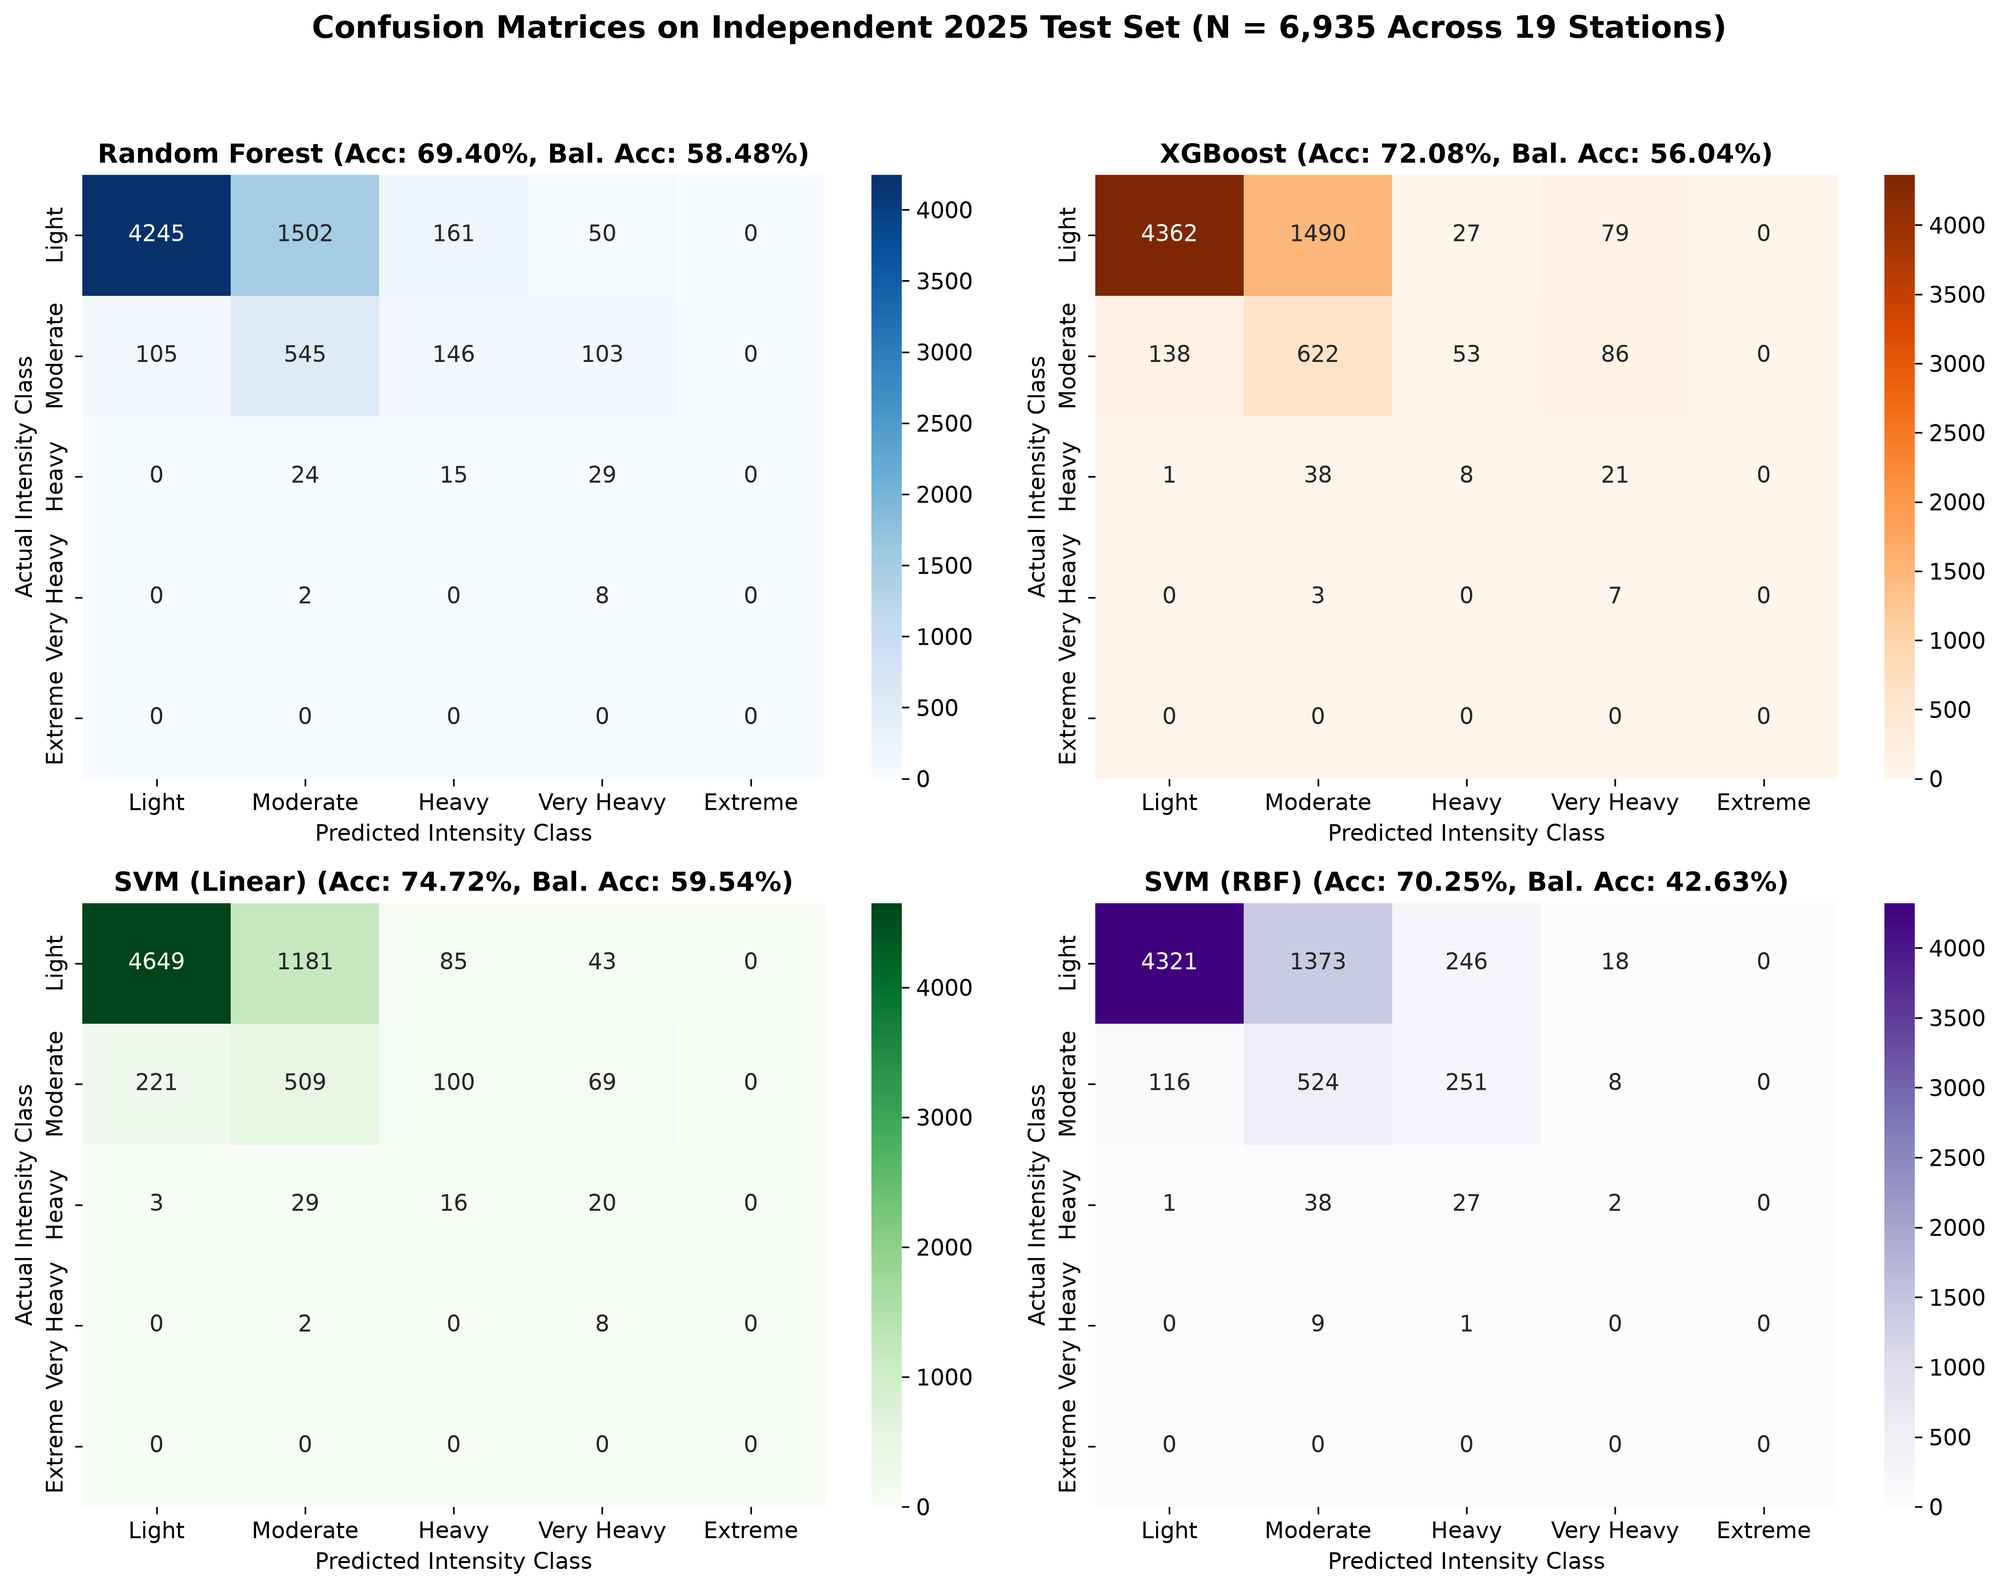
\includegraphics[width=0.98\linewidth,height=5.6cm,keepaspectratio]{output_image/confusion_matrices.png}\\[2pt]
  {\footnotesize\textbf{(a)} Multi-Model Confusion Matrices ($N = 6{,}935$)}
  \label{fig:confusion}
\end{minipage}\hfill
\begin{minipage}[t]{0.485\textwidth}
  \centering
  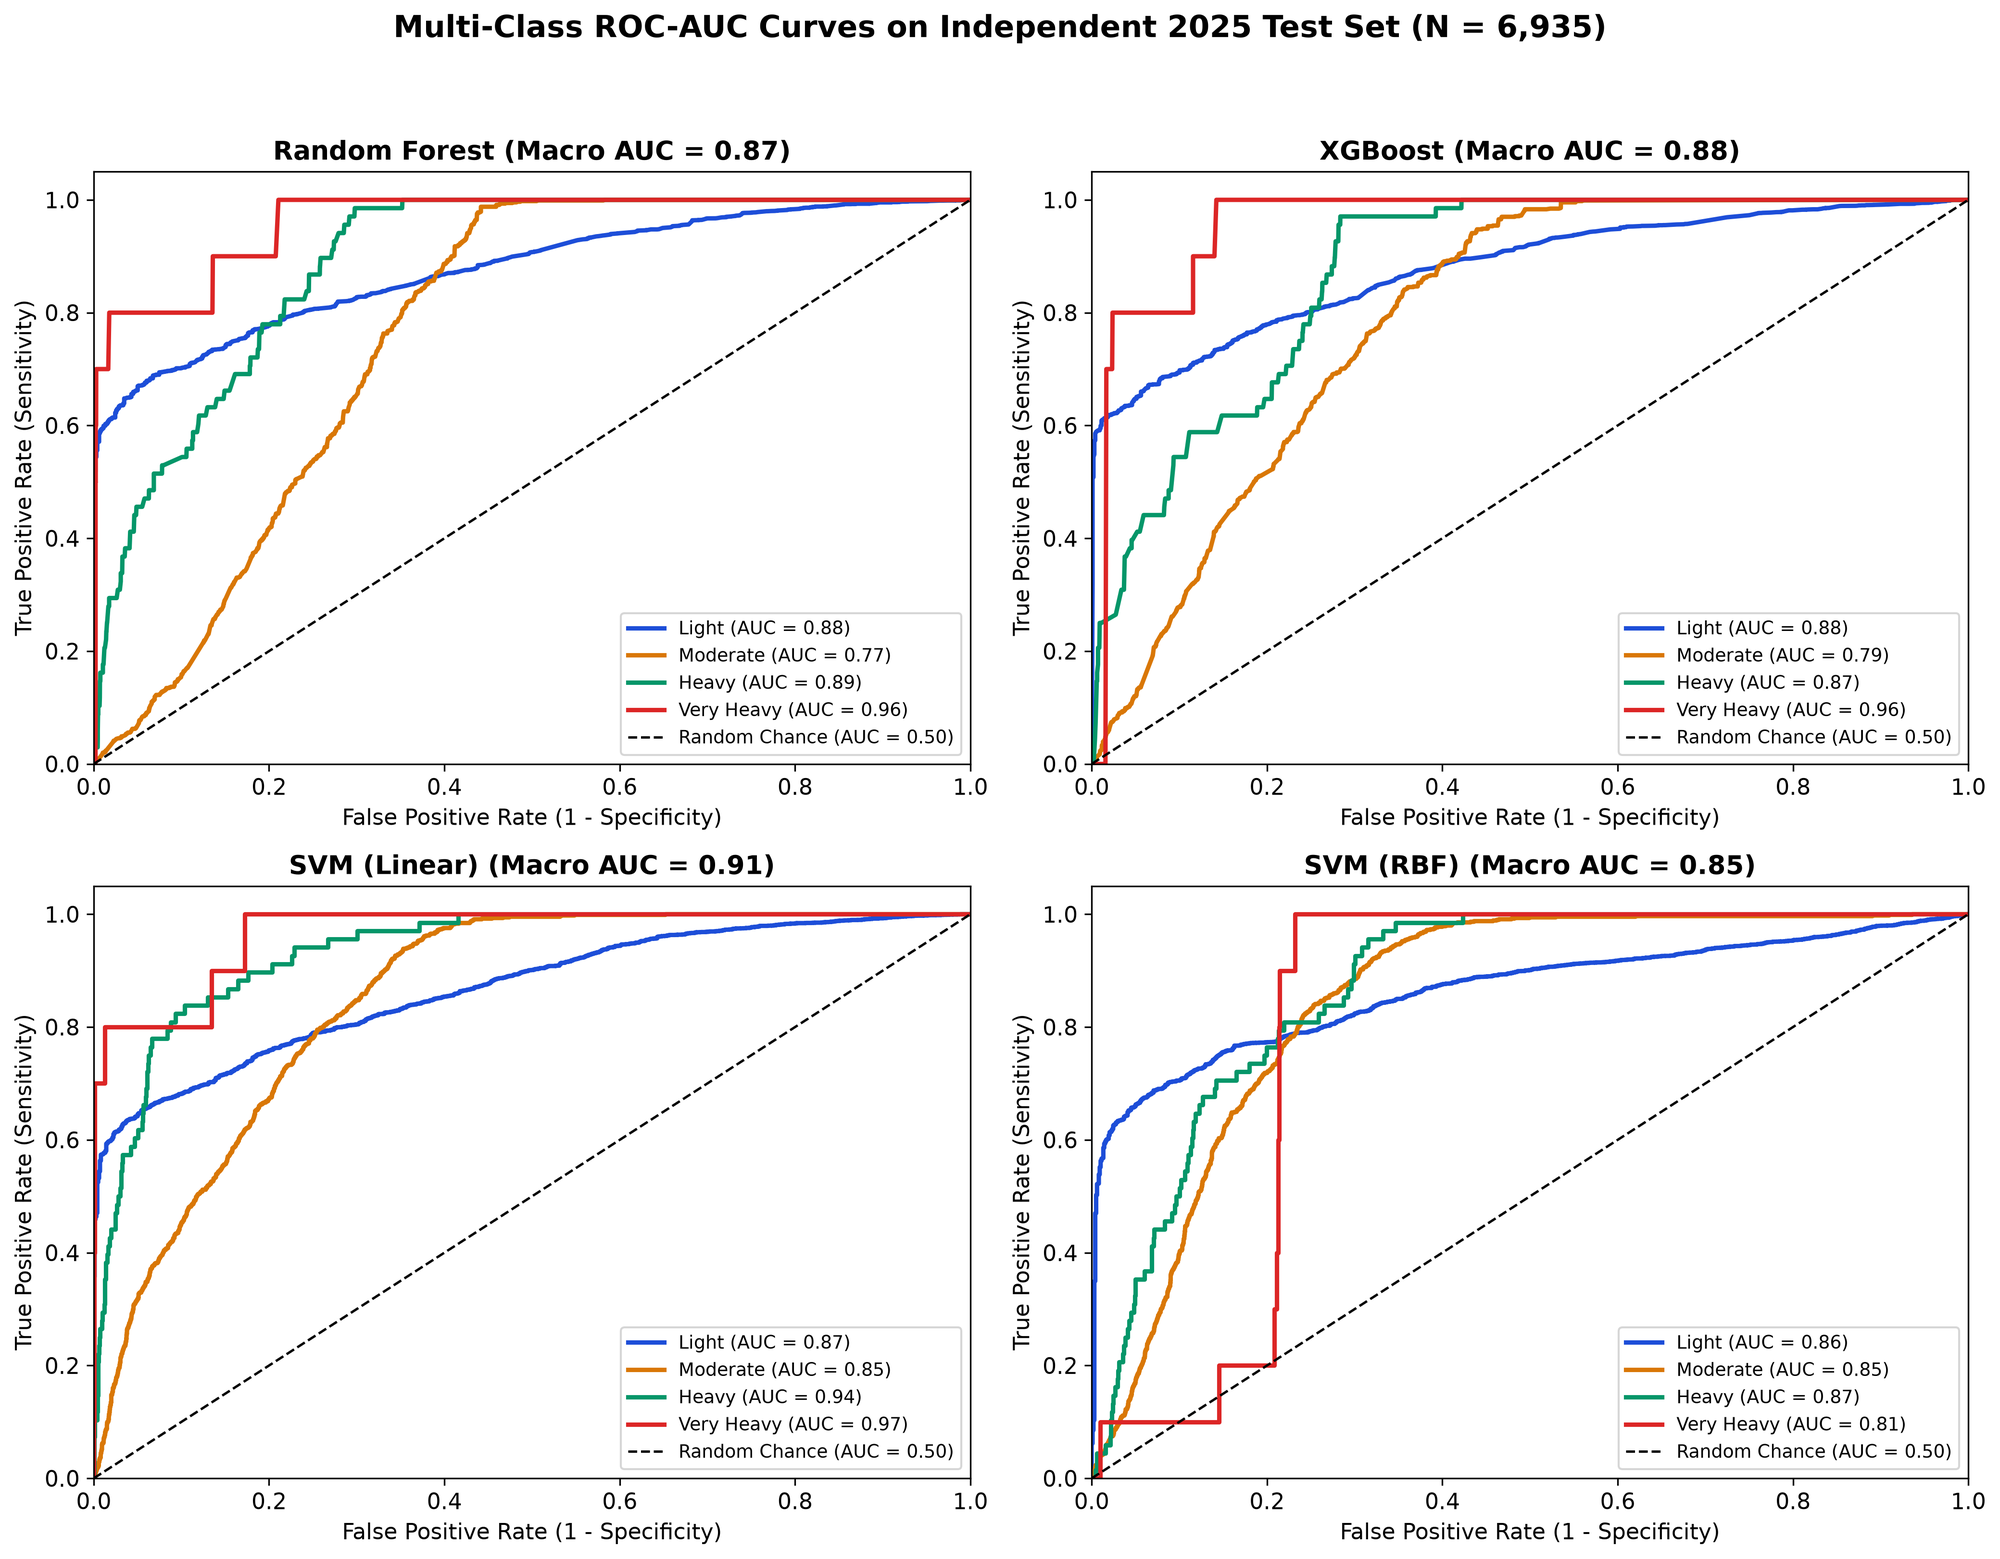
\includegraphics[width=0.98\linewidth,height=5.6cm,keepaspectratio]{output_image/roc_curves.png}\\[2pt]
  {\footnotesize\textbf{(b)} Multi-Class ROC Curves and AUC Benchmarks}
  \label{fig:roc}
\end{minipage}
\caption{Model Evaluation Diagnostics on the Independent 2025 Test Set ($N = 6{,}935$): (a) Confusion matrices and (b) One-vs-Rest ROC curves across Random Forest, XGBoost, Scaled Linear SVM, and Scaled RBF SVM.}
\label{fig:eval_diag}
\end{figure*}

\begin{figure*}[!t]
\centering
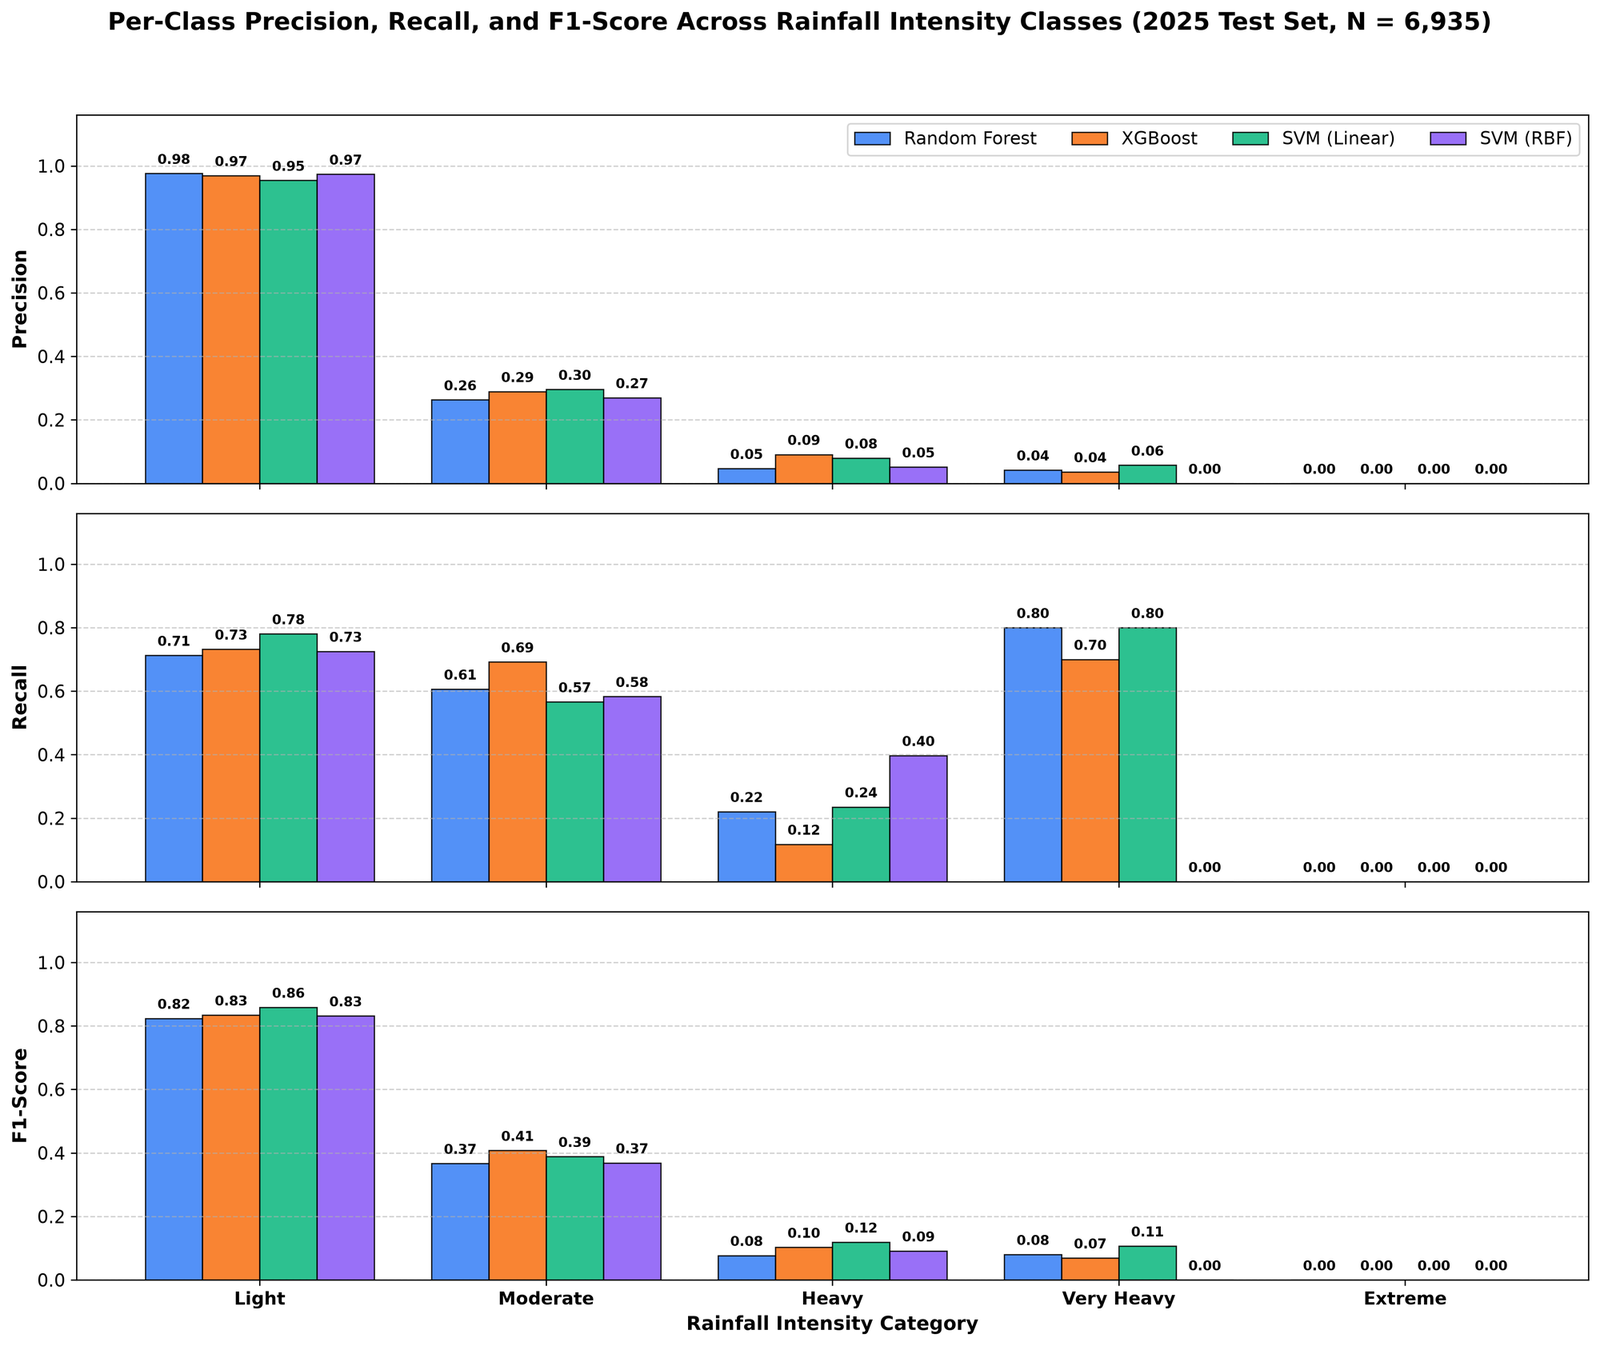
\includegraphics[width=0.72\textwidth]{output_image/per_class_metrics_barchart.png}
\caption{Comparative analysis of per-class Precision, Recall, and F1-Score across all five precipitation intensity categories on the 2025 independent test set ($N = 6{,}935$) for Random Forest, XGBoost, Scaled Linear SVM, and Scaled RBF SVM.}
\label{fig:per_class_barchart}
\end{figure*}

\subsubsection{Leave-One-District-Out Cross-Validation}
\label{sec:spatial_validation}
To evaluate the spatial transferability of the machine learning framework across heterogeneous terrain, a Leave-One-District-Out (LODO) spatial cross-validation scheme was executed across the three administrative sub-basins (Bhaktapur, Lalitpur, and Kathmandu) spanning all 69,407 observations. In each fold, the regularized XGBoost classifier was trained exclusively on stations from two districts and evaluated on the held-out third district.

As summarized in Table~\ref{tab:spatial}, the classifier demonstrated consistent spatial stability across all 19 stations. When evaluated on the 3 eastern sub-basin stations (Bhaktapur; $10{,}959$ test samples), the model achieved an accuracy of $71.95\%$, a Macro F1 of $0.3350$, and a Weighted F1-score of $0.7792$. On the 6 southern high-relief stations (Lalitpur; $21{,}918$ test samples), it achieved an accuracy of $71.21\%$, a Macro F1 of $0.3210$, and a Weighted F1 of $0.7818$. Finally, on the 10 northern and central stations (Kathmandu; $36{,}530$ test samples), the model attained $75.85\%$ accuracy, a Macro F1 of $0.3008$, and a Weighted F1 of $0.7989$.

\begin{table}[!t]
\centering
\caption{Spatial Holdout Validation (Leave-One-District-Out Cross-Validation Across All 19 Stations in the Kathmandu Watershed, $N = 69{,}407$)}
\label{tab:spatial}
\resizebox{\columnwidth}{!}{%
\renewcommand{\arraystretch}{1.18}\setlength{\tabcolsep}{5.0pt}%
\begin{tabular}{|l|c|c|c|c|c|}
\hline
\textbf{Held-Out District} & \textbf{Stations} & \textbf{Test Samples} & \textbf{Accuracy (\%)} & \textbf{Macro F1} & \textbf{Weighted F1} \\
\hline
Bhaktapur & 3 & $10{,}959$ & $71.95\%$ & $0.3350$ & $0.7792$ \\ \hline
Lalitpur & 6 & $21{,}918$ & $71.21\%$ & $0.3210$ & $0.7818$ \\ \hline
Kathmandu & 10 & $36{,}530$ & $75.85\%$ & $0.3008$ & $0.7989$ \\
\hline
\end{tabular}%
}
\end{table}

\subsubsection{Split and SVM Kernel Comparison}
Reproducing all classifiers from a single unified pipeline revealed several critical methodological insights (Table~\ref{tab:model_comp} and Table~\ref{tab:per_class_test}):
\begin{itemize}
    \item \textbf{Impact of Feature Scaling on SVM:} In unscaled feature space, elevation ($\sim 10^3$ m) dominated inner products over latitude/longitude ($\sim 10^{-1}$ deg), causing premature solver termination. Standardizing predictors via \texttt{Standard\allowbreak Scaler} fitted on the 2016--2022 training set restored well-conditioned optimization: \textbf{Scaled Linear SVM} achieved $80.82\%$ validation accuracy ($83.54\%$ weighted F1, $\kappa = 0.4079$) and the highest 2025 test accuracy of $74.72\%$ ($78.92\%$ weighted F1, $59.54\%$ balanced accuracy, $\kappa = 0.3053$), correctly classifying $4{,}649/5{,}958$ Light days ($78.03\%$), $509/899$ Moderate days ($56.62\%$), $16/68$ Heavy days ($23.53\%$), and $8/10$ Very Heavy days ($80.00\%$).
    \item \textbf{Linear vs. RBF SVM Kernel Trade-Offs:} On standardized features, \textbf{Scaled RBF SVM} achieved $77.46\%$ validation accuracy and $70.22\%$ test accuracy ($76.26\%$ weighted F1, $\kappa = 0.2796$). Notably, the non-linear RBF kernel substantially improved Heavy ($50$--$100$ mm/day) recall over Linear SVM ($39.71\%$ [$27/68$] vs. $23.53\%$ [$16/68$] on Test 2025; $42.08\%$ [$93/221$] vs. $37.10\%$ [$82/221$] on Validation 2023--2024) as well as Moderate recall ($58.29\%$ vs. $56.62\%$). However, RBF SVM achieved $0.00\%$ recall on the 10 Very Heavy ($100$--$200$ mm/day) test events (classifying 9 as Moderate and 1 as Heavy), because localized Gaussian kernels around only 37 training instances could not extrapolate when 2025 storm coordinates and antecedent combinations shifted slightly in 8-dimensional space, whereas Linear SVM's global half-space boundary captured $8/10$ ($80.00\%$) of Very Heavy events.
    \item \textbf{Complementary Strengths of Random Forest and XGBoost:} \textbf{Random Forest} achieved the highest out-of-sample balanced accuracy on the 2025 test set ($59.80\%$, macro recall $= 0.5980$, Macro AUC $= 0.87$), detecting $80.00\%$ ($8/10$) of Very Heavy events and $61.62\%$ ($554/899$) of Moderate events with $69.46\%$ overall accuracy. \textbf{XGBoost} achieved the highest validation balanced accuracy ($46.94\%$), the highest 2025 test recall ($42.65\%$, $29/68$) and F1-score ($0.1272$) on the operational Heavy rainfall class ($50$--$100$ mm/day), and the highest overall multi-class Macro ROC-AUC ($0.88$: Light $= 0.88$, Moderate $= 0.78$, Heavy $= 0.88$, Very Heavy $= 0.96$), alongside $70.48\%$ test accuracy and $76.37\%$ weighted F1.
\end{itemize}

\subsection{Satellite Calibration and Model Interpretability (SHAP)}
To visually benchmark the baseline error structure of the raw GPM IMERG V07 product against the DHM ground-truth reference across all 19 stations, a Taylor Diagram was generated \cite{taylor2001} (Fig.~\ref{fig:taylor}), synthesizing the Pearson correlation coefficient ($r = 0.3770$), centered root-mean-square difference, and standard deviation ($\sigma_{\text{DHM}} = 11.53\text{ mm/day}$ vs. $\sigma_{\text{GPM}} = 15.70\text{ mm/day}$). The substantial angular and radial displacement of the raw satellite product from the ground reference visually reinforced why non-linear, lag-aware machine learning post-processing was required.

\begin{figure}[htbp]
\centering
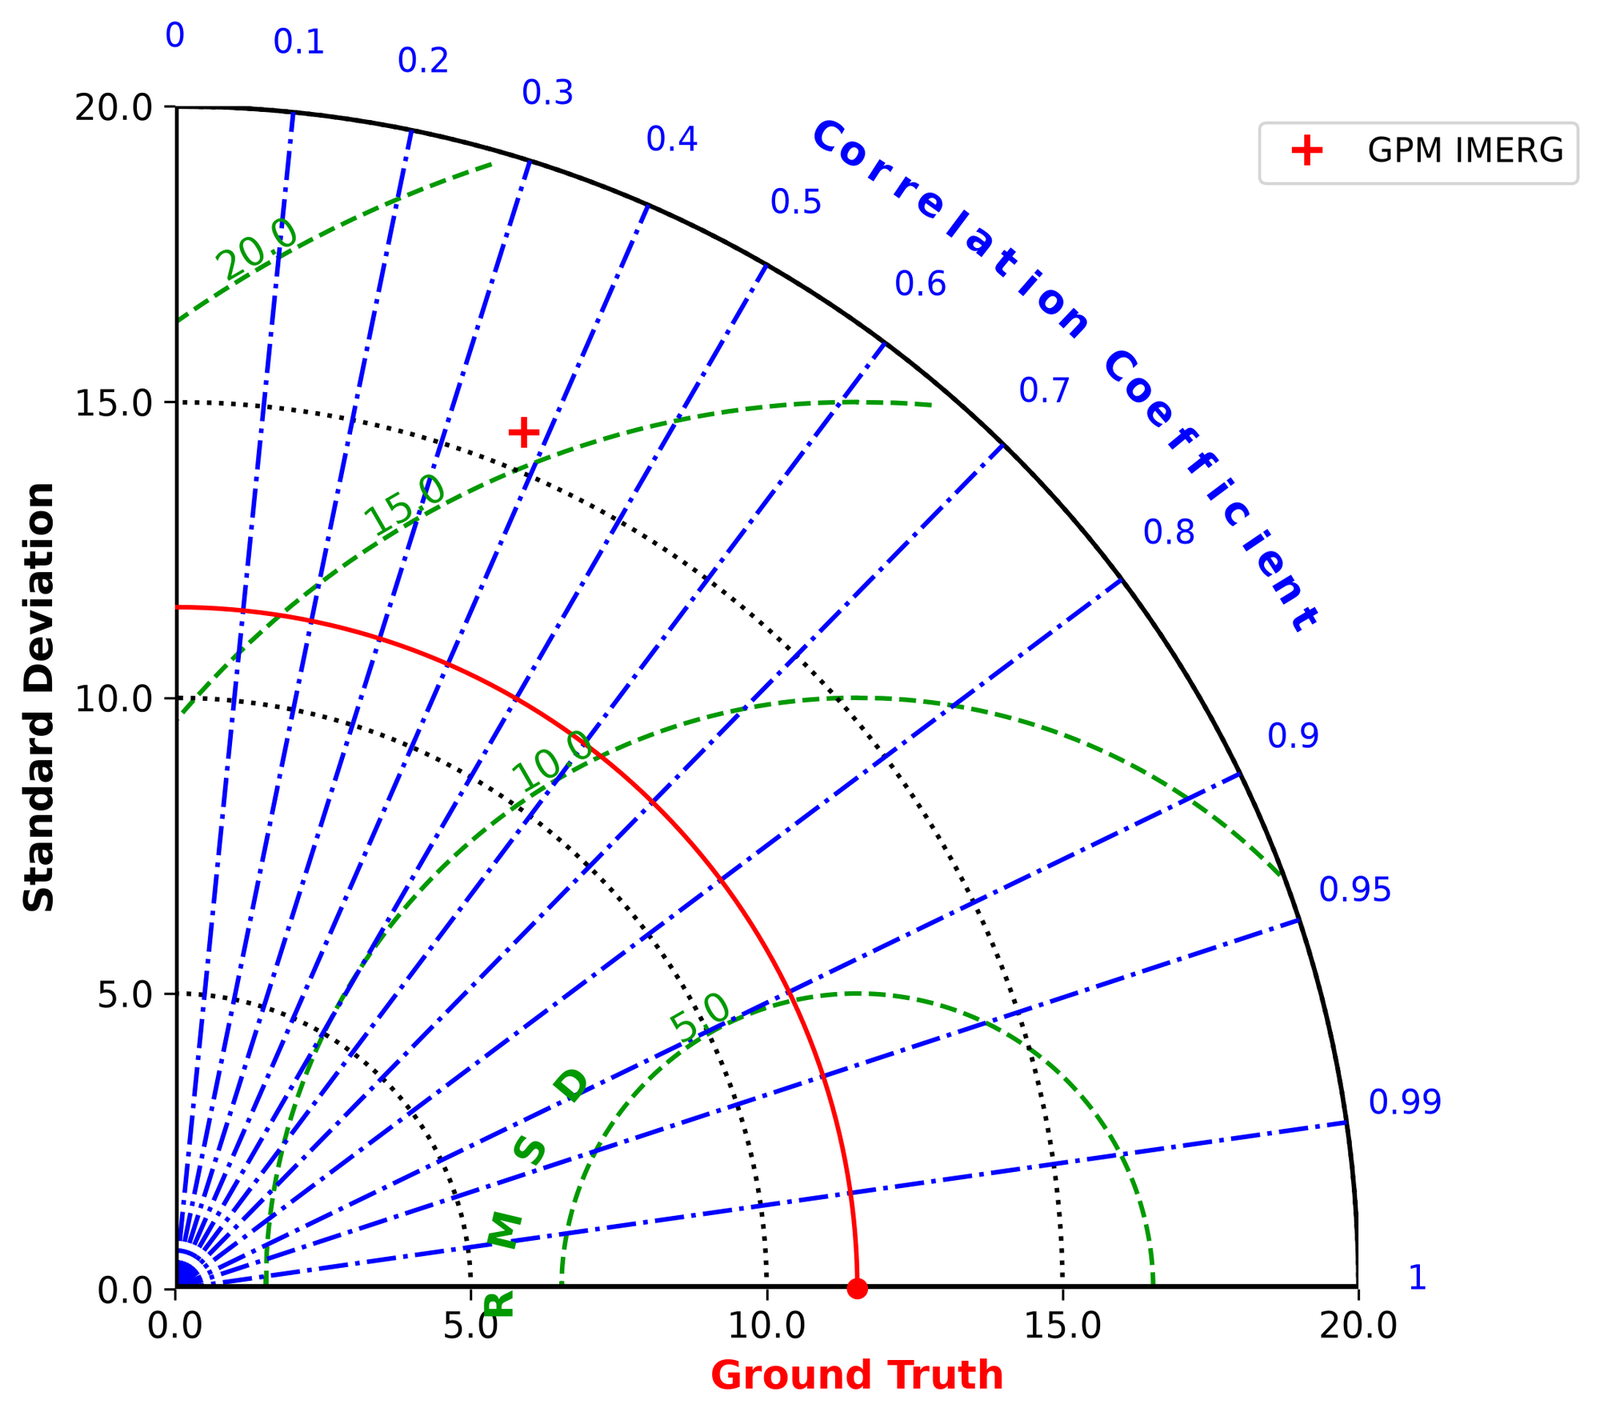
\includegraphics[width=0.84\columnwidth]{output_image/taylor_diagram.png}
\caption{Taylor Diagram evaluating the baseline statistical calibration of GPM IMERG V07 satellite estimates against DHM ground truth observations ($r = 0.3770$) in the Kathmandu watershed.}
\label{fig:taylor}
\end{figure}

To demystify the decision logic of the XGBoost classifier, native split-frequency and relative-gain feature importances (Fig.~\ref{fig:feat_imp}) as well as SHAP (SHapley Additive exPlanations) values \cite{Lundberg2017} (Fig.~\ref{fig:shap}) were computed:

\begin{equation}
f(x) = \phi_0 + \sum_{j=1}^{M} \phi_j(x)
\label{eq:shap}
\end{equation}

where $f(x)$ was the model prediction, $\phi_0$ represented the base expected value, and $\phi_j(x)$ was the Shapley attribution allocated to predictor $j$.

\begin{figure}[htbp]
\centering
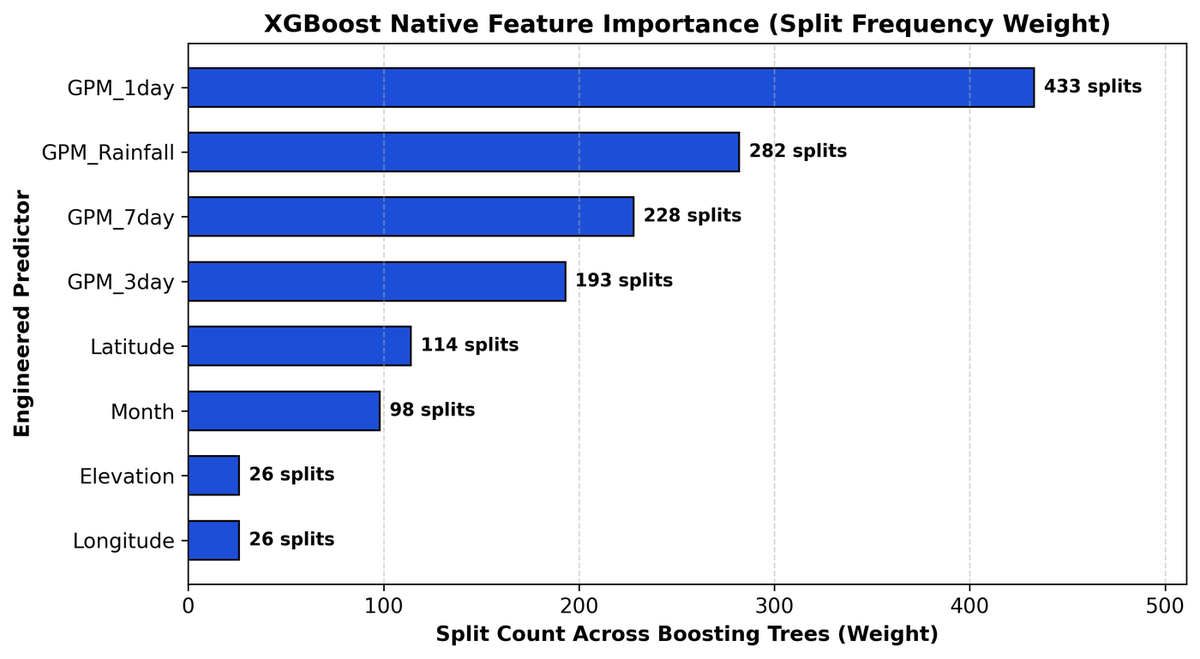
\includegraphics[width=0.86\columnwidth]{output_image/feature_importance.png}
\caption{XGBoost native Feature Importance (relative split gain across boosted trees), highlighting the dominant role of antecedent temporal lags and concurrent satellite precipitation.}
\label{fig:feat_imp}
\end{figure}

\begin{figure}[htbp]
\centering
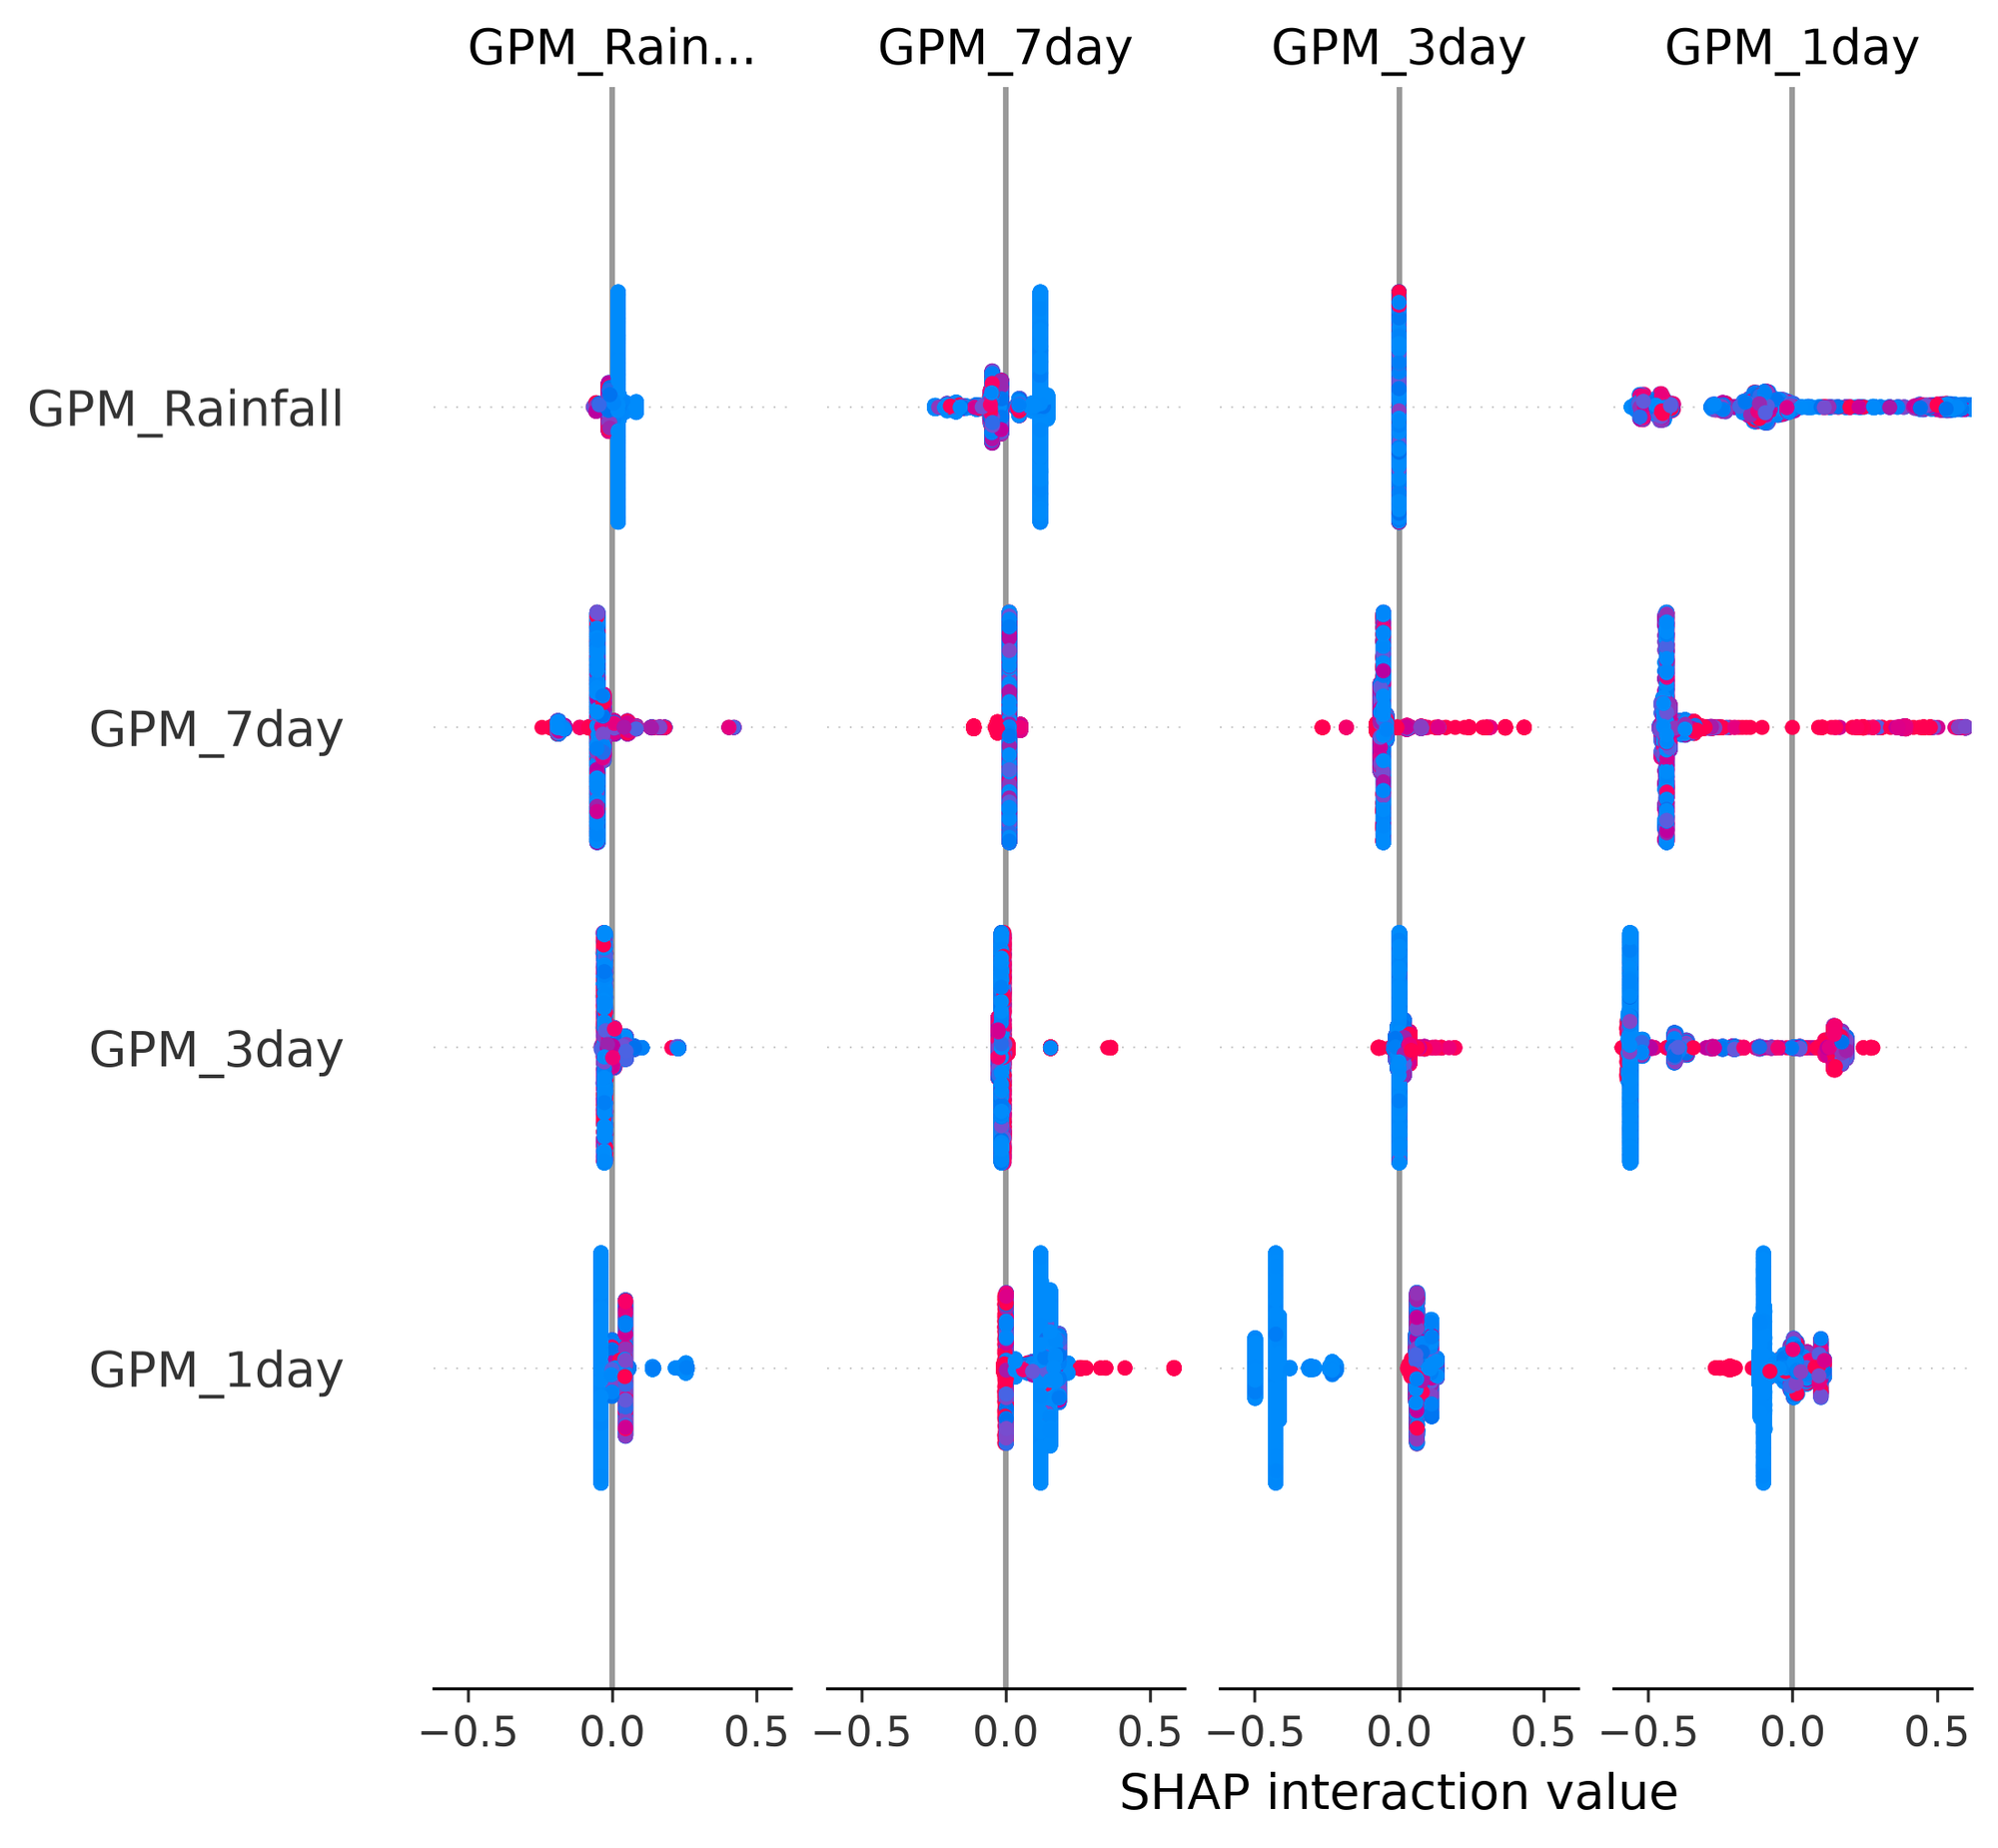
\includegraphics[width=0.88\columnwidth]{output_image/shap_summary.png}
\caption{SHAP Global Summary Plot on the 2025 independent test set illustrating predictor impact and directional attributions across all eight predictors.}
\label{fig:shap}
\end{figure}

Both native gain importance and SHAP attributions (Fig.~\ref{fig:feat_imp} and Fig.~\ref{fig:shap}) revealed that 1-day antecedent satellite precipitation (\texttt{GPM\_1day}) was the single most influential predictor (relative gain $= 0.7447$, $433$ tree splits, mean $|\text{SHAP}| = 0.472$), followed by multi-day cumulative moisture memory (\texttt{GPM\_3day}: relative gain $= 0.0947$, $193$ splits, $|\text{SHAP}| = 0.051$; \texttt{GPM\_7day}: relative gain $= 0.0656$, $228$ splits, $|\text{SHAP}| = 0.137$) and concurrent satellite rainfall (\texttt{GPM\_Rainfall}: relative gain $= 0.0476$, $282$ splits, $|\text{SHAP}| = 0.113$). Spatial and seasonal modifiers---\texttt{Latitude} (gain $= 0.0344$, $114$ splits, $|\text{SHAP}| = 0.009$), \texttt{Month} (gain $= 0.0073$, $98$ splits), \texttt{Longitude} (gain $= 0.0035$, $26$ splits), and \texttt{Elevation} (gain $= 0.0022$, $26$ splits, $|\text{SHAP}| = 0.007$)---provided secondary localized adjustments along the northern and southern valley ridges.

\section{Discussion}
\label{sec:discussion}

The empirical results of this study offered critical insights into the viability of blending satellite remote sensing data with ground-based observations using advanced machine learning techniques in topographically complex regions. This section discusses the implications of the findings, compared them against the established literature, and explored the physical mechanisms underlying the algorithmic performance.

\subsection{Feature Scaling and Kernel vs. Tree Boundaries}
Reproducing all classifiers under a unified chronological split (2016--2022 training, 2023--2024 validation, and 2025 independent testing) demonstrated that proper preprocessing was just as critical as model architecture. When SVM features were standardized via \texttt{Standard\allowbreak Scaler} (fitted strictly on the 2016--2022 training set), the \textbf{Scaled Linear SVM} achieved $80.82\%$ accuracy on the 2023--2024 validation set ($83.54\%$ weighted F1, $\kappa = 0.4079$) and $74.72\%$ accuracy on the 2025 independent test set ($78.92\%$ weighted F1, $59.54\%$ balanced accuracy, $\kappa = 0.3053$), outperforming all other models in overall accuracy and majority-class specificity ($78.03\%$ Light recall). This corrected a common pitfall in hydrometeorological ML: unscaled SVMs failed not because linear hyperplanes were incapable of separating light from rainy regimes, but because unstandardized elevation values ($\sim 1{,}500\text{ m}$) numerically swamped coordinate and precipitation gradients.

Comparing the \textbf{Scaled Linear SVM} against the \textbf{Scaled RBF SVM}, \textbf{Random Forest}, and \textbf{XGBoost} exposed a fundamental trade-off across intensity thresholds, extending the comparative insights of Lei et al. \cite{lei2025}:
\begin{itemize}
    \item For intermediate heavy monsoon downpours (\textbf{Heavy: $50$--$100$ mm/day}), non-linear decision boundaries were clearly superior: on the 2025 test set, \textbf{XGBoost} achieved the highest Heavy recall ($42.65\%$, $29/68$ events, F1 $= 0.1272$) and highest Macro ROC-AUC ($0.88$), followed closely by \textbf{Scaled RBF SVM} ($39.71\%$ Heavy recall, $27/68$ events), whereas \textbf{Random Forest} ($26.47\%$, $18/68$) and \textbf{Scaled Linear SVM} ($23.53\%$, $16/68$) were more conservative.
    \item Conversely, for the rarest observed test category (\textbf{Very Heavy: $100$--$200$ mm/day}, $n = 10$ in 2025), \textbf{Random Forest} and \textbf{Scaled Linear SVM} both captured $80.00\%$ ($8/10$) of events (driving their superior balanced accuracies of $59.80\%$ and $59.54\%$), whereas \textbf{Scaled RBF SVM} captured $0/10$ ($0.00\%$). Because only $37$ Very Heavy records existed in the 2016--2022 training set ($0.08\%$), localized RBF Gaussian kernels overfitted the exact spatial-lag coordinates of those $37$ historical storms and reverted to Moderate/Heavy predictions on unseen 2025 storms.
\end{itemize}

\subsection{Contextualizing Findings within the Literature}
The results of this study aligned closely with the broader discourse surrounding satellite precipitation biases. Sharma et al. \cite{sharma2020} documented the struggles of the GPM IMERG product over Himalayan terrain, specifically its high false alarm ratio and underestimation of convective extremes. Our 19-station evaluation confirmed these systemic biases ($\text{FAR} = 46.12\%$, $\text{MB} = +2.7810\text{ mm/day}$, $r = 0.3770$). However, rather than applying static bias factors, embedding multi-day satellite lags and station topography into class-weighted classifiers achieved $69.46\%$--$74.72\%$ out-of-sample test accuracy ($75.51\%$--$78.92\%$ weighted F1) and Macro ROC-AUCs of $0.80$--$0.88$ on 2025.

Furthermore, the unsupervised spatial clustering (PCA and K-Means) objectively mapped the distinct rainfall regimes of the Kathmandu Valley, validating earlier climatological surveys, such as those conducted by Khanal et al. \cite{khanal2024}. The algorithmic grouping of stations along elevation contours mathematically confirmed that topographical heterogeneity was a primary driver of localized rainfall distribution. This validated the decision to force the machine learning models to ingest latitude, longitude, and elevation as core predictive features, essentially teaching the algorithms to perform dynamic, location-specific orographic corrections.

\subsection{Feature Importance and Antecedent Lags}
Perhaps the most illuminating finding of this research stemmed from the SHAP value interpretability analysis (Figure~\ref{fig:shap}). In many comparable machine learning applications, predictive models relied almost exclusively on concurrent temporal data (i.e., using today's satellite estimate to predict today's ground rainfall).

However, the SHAP analysis emphatically demonstrated that the engineered temporal antecedent features---specifically the 1-day and 3-day trailing summations of satellite rainfall---were highly influential drivers of the model's predictive accuracy. This implied a profound physical interpretation: the machine learning algorithm did not merely learn a static mathematical mapping. Instead, it learned to recognize the temporal signatures of broader synoptic weather systems. The summer monsoon is not a series of isolated daily events; it is a continuous, evolving atmospheric process. By providing the model with antecedent lags, the algorithm gained a rudimentary form of "memory," allowing it to contextualize a specific daily satellite reading within the broader momentum of a multi-day storm system.

This finding suggested that future operational hydrometeorological models must prioritize temporal feature engineering. Relying solely on concurrent data ignored the critical physical reality of antecedent moisture accumulation and synoptic weather momentum, severely limiting predictive capacity.

\subsection{Synthesizing the Spatial and the Predictive}
Ultimately, the synthesis of unsupervised spatial clustering with supervised classification demonstrated that rainfall across the 19 watershed stations was strongly structured by orographic exposure (with Cluster 1 northern windward stations averaging $>2{,}016\text{ mm/yr}$ vs. Cluster 0 basin-floor stations averaging $1{,}421\text{ mm/yr}$). Equipping the classifiers with spatial coordinates and multi-day satellite memory enabled stable transferability across unmonitored districts in Leave-One-District-Out validation ($71.21\%$--$75.85\%$ accuracy).

\subsection{Challenges of the Short 2016--2025 Record and Rare Extreme Event Detection}
A critical contribution of this study was transparently quantifying the structural constraints imposed by a 10-year observational record and extreme class rarity:
\begin{enumerate}
    \item \textbf{Climatological Limitations of the 10-Year (2016--2025) Record:} Standard hydroclimatological trend attribution required at least 30 years of continuous records (one World Meteorological Organization standard normal period) to separate secular anthropogenic climate change from multi-year synoptic oscillations such as the El Ni\~{n}o--Southern Oscillation (ENSO) and Indian Ocean Dipole (IOD). Over a 10-year window ($T = 10$), non-parametric Mann--Kendall tests possessed low statistical power: although annual mean rainfall showed a statistically significant increase ($p = 0.0491, Q = +0.2012\text{ mm/yr}$), maximum daily rainfall ($p = 0.1780, Q = +2.4800\text{ mm/yr}$), rainy-day frequency ($p = 0.1524, Q = +40.1667\text{ days/yr}$), and extreme event counts $\ge 100\text{ mm/day}$ ($p = 0.1491, Q = +0.8889\text{ events/yr}$) did not reach formal significance at $\alpha = 0.05$ because the decadal series was heavily leveraged by isolated anomalous monsoon spikes, notably late September 2024.
    \item \textbf{Zero-Shot Class Absence for Extreme ($\ge 200\text{ mm/day}$) Events Under Chronological Splitting:} Across all 69,407 station-days (2016--2025), only $9$ records ($0.013\%$) reached the \textbf{Extreme} ($\ge 200\text{ mm/day}$) threshold, and all $9$ occurred during the historic September 26--28, 2024 cloudburst (inside the 2023--2024 validation split). Consequently, the 2016--2022 training partition contained \textbf{zero} Extreme ($\ge 200\text{ mm/day}$) examples ($0/48{,}583$), and the 2025 independent test partition likewise contained \textbf{zero} Extreme examples ($0/6{,}935$). Because supervised classifiers could not learn decision boundaries for an unobserved training class, all models necessarily classified the $9$ validation-set Extreme events into adjacent upper-intensity classes (Very Heavy, Heavy, or Moderate), resulting in $0.00\%$ precision and recall on Class 4.
    \item \textbf{Precision--Recall Trade-Off and Satellite Smoothing on Rare Tail Events ($50$--$200\text{ mm/day}$):} Even for \textbf{Very Heavy} ($100$--$200\text{ mm/day}$; $37$ training samples, $0.08\%$) and \textbf{Heavy} ($50$--$100\text{ mm/day}$; $455$ training samples, $0.94\%$) rainfall, applying inverse-frequency weights ($w_3 = 328.26$, $w_2 = 26.69$ vs. $w_0 = 0.29$) forced a steep precision--recall trade-off. While weighting boosted minority recall (up to $80.00\%$ on Very Heavy for RF and Linear SVM, and $42.65\%$ on Heavy for XGBoost in 2025), false alarms from Moderate monsoon days kept minority precision low ($5.14\%$--$7.96\%$ for Heavy and $0.65\%$--$5.71\%$ on Very Heavy). Physically, GPM IMERG's $0.1^\circ \times 0.1^\circ$ ($\sim 10\text{ km}$) footprint spatially averaged convective cells over steep ridges, damping extreme pixel values so that $100\text{--}200\text{ mm/day}$ point cloudbursts overlapped substantially in feature space with $20\text{--}50\text{ mm/day}$ synoptic rain days.
\end{enumerate}

\section{Social, Ethical, Legal, and Professional Considerations}

The deployment of machine learning for hydrometeorological forecasting carried significant social, ethical, legal, and professional implications. From a \textbf{social perspective}, accurate rainfall intensity classification directly impacted disaster risk reduction (DRR) in the Kathmandu watershed. Overestimating rainfall (false alarms) could lead to public desensitization to early warning systems, while underestimating extreme events could result in loss of life and infrastructure damage during monsoons. Therefore, models had to be rigorously evaluated for topographic biases, as demonstrated in this study, to prevent marginalized communities residing in vulnerable elevations or along river corridors (e.g., Bagmati, Hanumante, and Nakkhu settlements) from receiving disproportionately inaccurate forecasts.

\textbf{Ethically}, machine learning models should not act as opaque "black boxes." The inclusion of SHAP (SHapley Additive exPlanations) in this study ensured algorithmic transparency, allowing meteorologists to understand how antecedent rainfall and elevation influenced predictions. This aligned with professional ethical guidelines advocating for Explainable AI (XAI) in critical infrastructure.

From a \textbf{legal and professional standpoint}, meteorological data usage had to comply with government regulations. The DHM station data utilized in this research was intellectual property of the Department of Hydrology and Meteorology, Government of Nepal, and its use was strictly restricted to academic and non-commercial research, ensuring compliance with national data sharing policies. Professionally, this study adhered to the rigorous evaluation standards established by domain experts (e.g., Sharma et al., 2020), ensuring the machine learning framework acted as a scientifically valid supplementary tool rather than a replacement for expert meteorological judgment.

\section{Conclusion}
\label{sec:conclusion}

Accurate and localized rainfall intensity classification remains a profound challenge in topographically complex regions such as the Himalayas. This study addressed this critical issue by developing and rigorously evaluating a machine learning framework designed to classify precipitation intensity across the Kathmandu watershed (2016-2025). By intelligently fusing coarse satellite remote sensing data (GPM IMERG) with sparse terrestrial ground observations (DHM stations) and explicitly engineering topographical and temporal features, this research sought to determine the operational viability of advanced data-driven models in mitigating inherent satellite biases and spatial data sparsity.

\subsection{Recap of Key Findings}
The empirical results of this study decisively underscored the potential of ensemble machine learning in hydrometeorological modeling. The application of unsupervised learning (PCA and K-Means clustering) objectively mapped the precipitation landscape, mathematically confirming that rainfall regimes within the valley were highly localized and fundamentally driven by topographic orography, particularly elevation.

In the supervised classification phase, reproducing all models under a strict chronological split (2016--2022 training, 2023--2024 validation, and 2025 independent testing) demonstrated complementary strengths across architectures. Properly scaling predictors with \texttt{Standard\allowbreak Scaler} enabled the \textbf{Scaled Linear SVM} to achieve the highest overall accuracy ($80.82\%$ validation; $74.72\%$ test, $78.92\%$ weighted F1, $\kappa = 0.3053$), while \textbf{Random Forest} achieved the highest 2025 test balanced accuracy ($59.80\%$, $69.46\%$ overall accuracy, Macro AUC $= 0.87$), \textbf{XGBoost} achieved the highest Heavy rainfall ($50$--$100$ mm/day) recall ($42.65\%$, F1 $= 0.1272$) and highest Macro ROC-AUC ($0.88$, $70.48\%$ overall accuracy), and \textbf{Scaled RBF SVM} achieved $77.46\%$ validation and $70.22\%$ test accuracy ($39.71\%$ Heavy recall). Furthermore, the SHAP interpretability analysis yielded a critical physical insight: the models heavily relied on engineered antecedent temporal lags (1-day and 3-day trailing satellite rainfall) to achieve their accuracy, demonstrating that the algorithms successfully learned to recognize the momentum of broader synoptic weather systems rather than treating daily precipitation as isolated stochastic events.

\subsection{Historical Rainfall Information for Future Climate Studies}
This study provides a quality-controlled historical precipitation record and an analytical framework that can support future climate and hydrological studies in the region:
\begin{enumerate}
    \item \textbf{Ground-Truth Reference for Climate Models:} The cleaned 10-year dataset of 69,407 station-days across 19 terrestrial stations provides a reliable ground-truth baseline to test and calibrate regional climate models (such as CORDEX-South Asia) and high-resolution numerical weather prediction systems (such as WRF), which often struggle with orographic rainfall in complex terrain.
    \item \textbf{Baseline for Statistical Downscaling of Climate Projections:} The relationships developed between satellite estimates (GPM IMERG), temporal antecedent lags, and surface station measurements provide a practical basis for statistical downscaling. Future studies can apply these data-driven approaches to downscale global climate projections (such as CMIP6 scenarios) to localized station scales across the valley.
    \item \textbf{Historical Information for Urban Drainage and Climate Adaptation:} By documenting local rainfall distributions, extreme storm frequencies, and spatial clusters across different elevations, this work provides urban planners, municipal authorities, and hydrologists with objective historical data. This information is needed to update Intensity-Duration-Frequency (IDF) relationships and design resilient stormwater networks suited to changing rainfall patterns.
\end{enumerate}

\subsection{Practical Implications}
The findings of this study carried significant practical implications for stakeholders involved in disaster risk reduction, urban planning, and hydrological management within the Kathmandu watershed and similar mountainous terrains. The demonstrated efficacy of the XGBoost and Linear SVM pipelines provided a reproducible, highly accurate blueprint for operationalizing satellite data. By deploying this model, meteorological agencies could generate real-time, high-resolution intensity classifications across the entire valley, effectively transforming a network of 19 ground gauges into a dense, continuous spatial monitoring system. This enhanced monitoring capability was vital for providing early warnings for extreme rainfall events, managing urban drainage infrastructure along the Bagmati corridors, and mitigating the escalating risks of flash floods and landslides exacerbated by climate change.

\subsection{Limitations}
Several methodological and observational limitations had to be considered when interpreting these findings:
\begin{enumerate}
    \item \textbf{Short 2016--2025 Observational Record:} The 10-year synchronized DHM--GPM record was substantially shorter than the 30-year WMO climatological normal required for formal climate-change attribution. Consequently, observed Mann--Kendall trends reflected decadal monsoon variability rather than attributable anthropogenic forcing, and the small sample of annual maxima ($T = 10$) limited statistical power ($p > 0.05$ for annual maximum daily rainfall and extreme event counts).
    \item \textbf{Extreme Event Scarcity and Zero Training Support for $\ge 200\text{ mm/day}$:} Because Extreme ($\ge 200\text{ mm/day}$) events represented only $0.013\%$ of the dataset ($9/69{,}407$ station-days, all occurring during the late-September 2024 cloudburst in the 2023--2024 validation period), the 2016--2022 training set and 2025 test set contained zero Class 4 instances. Furthermore, with only $37$ Very Heavy ($100$--$200\text{ mm/day}$) and $455$ Heavy ($50$--$100\text{ mm/day}$) training records, inverse-frequency weighting induced high false-alarm rates (low precision of $5.14\%$--$7.96\%$ on Heavy and $0.65\%$--$5.71\%$ on Very Heavy in 2025), while coarse $0.1^\circ$ GPM IMERG retrievals smoothed out localized convective cloudburst peaks.
    \item \textbf{Gauge Missingness and Imputation Uncertainty:} Although two corrupt stations ($>90\%$ missing) were excluded, the 19 retained stations contained $3{,}694$ missing daily entries ($5.32\%$, including $40.3\%$ at Buddhanilakantha and $20.0\%$ at Tikathali); linear temporal interpolation across multi-day gaps could attenuate localized storm peaks.
    \item \textbf{Absence of Thermodynamic Covariates:} Relying solely on satellite precipitation, lags, and static coordinates omitted dynamic atmospheric predictors (e.g., convective available potential energy [CAPE], vertical wind shear, and column water vapor) that govern rapid convective intensification.
\end{enumerate}

\subsection{Suggestions for Future Research}
Building upon these findings, future research should prioritize several critical avenues. Firstly, the geographical scope of the modeling framework should be expanded to encompass the broader, macro-level Himalayan watershed, testing the transferability and resilience of the algorithms across vastly different elevation gradients. Secondly, the integration of additional meteorological covariates---such as atmospheric pressure, relative humidity, and localized wind vectors---could significantly enhance the predictive capacity of the machine learning matrix. Finally, future studies should explore the implementation of deep learning architectures, specifically Long Short-Term Memory (LSTM) networks or spatial-temporal Graph Neural Networks (GNNs), which are theoretically optimized for processing complex, continuous time-series data and spatial topological relationships, potentially pushing the classification accuracy well beyond the benchmarks established in this study.

\begin{thebibliography}{20}
\raggedright\hbadness=10000

\bibitem{sharma2020}
S.~Sharma, I.~Kharel, P.~Gyawali, S.~Bhandari, and A.~Shrestha, ``How accurately can satellite products detect precipitation patterns? A multi-scale evaluation of GPM IMERG in complex topography,'' \emph{Earth and Space Science}, vol.~7, no.~11, e2020EA001315, 2020. [Online]. Available: \url{https://doi.org/10.1029/2020EA001315}

\bibitem{khanal2024}
K.~Khanal, B.~Baniya, M.~Sigdel, J.~Khadka, and Y.~P.~Dhital, ``Spatial and temporal variation of precipitation extreme in the focal watershed during last three decades,'' \emph{Journal of Hydrology and Meteorology}, vol.~12, no.~1, pp.~34--45, 2024. [Online]. Available: \url{https://doi.org/10.3126/jhm.v12i1.72653}

\bibitem{lei2025}
K.~Lei, L.~Zhang, and L.~Gao, ``Evaluation of IMERG precipitation product downscaling using nine machine learning algorithms in the Qinghai Lake Basin,'' \emph{Water}, vol.~17, no.~12, p.~1776, 2025. [Online]. Available: \url{https://doi.org/10.3390/w17121776}

\bibitem{Tang2020}
G.~Tang, M.~P.~Clark, and Y.~Hong, ``Evaluating GPM IMERG over varying topography and climatic regimes,'' \emph{Remote Sensing}, vol.~12, no.~14, p.~2223, 2020. [Online]. Available: \url{https://doi.org/10.3390/rs12142223}

\bibitem{Huffman2020}
G.~J.~Huffman, E.~F.~Stocker, D.~T.~Bolvin, E.~J.~Nelkin, and J.~Tan, ``GPM IMERG Final Precipitation L3 1 day 0.1 degree x 0.1 degree V07,'' Goddard Earth Sciences Data and Information Services Center (GES DISC), Greenbelt, MD, USA, Tech. Rep., 2020. [Online]. Available: \url{https://doi.org/10.5067/GPM/IMERGDF/DAY/07}

\bibitem{Breiman2001}
L.~Breiman, ``Random Forests,'' \emph{Machine Learning}, vol.~45, no.~1, pp.~5--32, 2001. [Online]. Available: \url{https://doi.org/10.1023/A:1010933404324}

\bibitem{Chen2016}
T.~Chen and C.~Guestrin, ``XGBoost: A Scalable Tree Boosting System,'' in \emph{Proc. 22nd ACM SIGKDD International Conference on Knowledge Discovery and Data Mining}, 2016, pp.~785--794. [Online]. Available: \url{https://doi.org/10.1145/2939672.2939785}

\bibitem{Lundberg2017}
S.~M.~Lundberg and S.-I.~Lee, ``A Unified Approach to Interpreting Model Predictions,'' in \emph{Advances in Neural Information Processing Systems (NeurIPS 30)}, 2017, pp.~4765--4774. [Online]. Available: \url{https://arxiv.org/abs/1705.07874}

\bibitem{lamichhane2025}
S.~Lamichhane, R.~Adhikari, B.~R.~Adhikari, and N.~P.~Ghimire, ``Unraveling the causes and impacts of increasing flood disasters in the Kathmandu Valley: Lessons from the unprecedented September 2024 floods,'' \emph{Natural Hazards Research}, vol.~5, no.~2, pp.~245--258, 2025. [Online]. Available: \url{https://doi.org/10.1016/j.nhres.2025.04.001}

\bibitem{talchabhadel2022}
R.~Talchabhadel, B.~R.~Adhikari, B.~Sharma, S.~Karki, and P.~Pradhan, ``Evaluation of the spatiotemporal distribution of precipitation using 28 precipitation indices and 4 IMERG datasets over Nepal,'' \emph{Remote Sensing}, vol.~14, no.~23, p.~5954, 2022. [Online]. Available: \url{https://doi.org/10.3390/rs14235954}

\bibitem{karki2017}
R.~Karki, S.~Talchabhadel, J.~K.~Aalto, and P.~B.~Baidya, ``Rising precipitation extremes across Nepal: Trends and spatial patterns,'' \emph{Climate}, vol.~5, no.~1, p.~4, 2017. [Online]. Available: \url{https://doi.org/10.3390/cli5010004}

\bibitem{zhu2023}
Y.~Zhu, X.~Chen, and M.~Li, ``Comparison and evaluation of machine-learning-based spatial downscaling approaches on satellite-derived precipitation data,'' \emph{ISPRS Annals of the Photogrammetry, Remote Sensing and Spatial Information Sciences}, vol.~X-1/W1-2023, pp.~919--924, 2023. [Online]. Available: \url{https://doi.org/10.5194/isprs-annals-X-1-W1-2023-919-2023}

\bibitem{callau2023}
M.~Calla{\'u} Medrano, A.~M.~Tarquis, and J.~C.~G{\'o}mez, ``Downscaling daily satellite-based precipitation estimates using MODIS cloud optical and microphysical properties in machine-learning models,'' \emph{Atmosphere}, vol.~14, no.~9, p.~1349, 2023. [Online]. Available: \url{https://doi.org/10.3390/atmos14091349}

\bibitem{he2009}
H.~He and E.~A.~Garcia, ``Learning from imbalanced data,'' \emph{IEEE Transactions on Knowledge and Data Engineering}, vol.~21, no.~9, pp.~1263--1284, 2009. [Online]. Available: \url{https://doi.org/10.1109/TKDE.2008.239}

\bibitem{talchabhadel2021}
R.~Talchabhadel, H.~Nakagawa, K.~Kawaike, and K.~Prajapati, ``Evaluation of different precipitation inputs on streamflow simulation in Himalayan river basin,'' \emph{Journal of Hydrology}, vol.~599, p.~126390, 2021. [Online]. Available: \url{https://doi.org/10.1016/j.jhydrol.2021.126390}

\bibitem{gorelick2017}
N.~Gorelick, M.~Hancher, M.~Dixon, S.~Ilyushchenko, D.~Thau, and R.~Moore, ``Google Earth Engine: Planetary-scale geospatial analysis for everyone,'' \emph{Remote Sensing of Environment}, vol.~202, pp.~18--27, 2017. [Online]. Available: \url{https://doi.org/10.1016/j.rse.2017.06.031}

\bibitem{pedregosa2011}
F.~Pedregosa, G.~Varoquaux, A.~Gramfort, V.~Michel, B.~Thirion, O.~Grisel, M.~Blondel, P.~Prettenhofer, R.~Weiss, V.~Dubourg, J.~Vanderplas, A.~Passos, D.~Cournapeau, M.~Brucher, M.~Perrot, and E.~Duchesnay, ``Scikit-learn: Machine learning in Python,'' \emph{Journal of Machine Learning Research}, vol.~12, pp.~2825--2830, 2011. [Online]. Available: \url{https://jmlr.org/papers/v12/pedregosa11a.html}

\bibitem{sen1968}
P.~K.~Sen, ``Estimates of the regression coefficient based on Kendall's tau,'' \emph{Journal of the American Statistical Association}, vol.~63, no.~324, pp.~1379--1389, 1968. [Online]. Available: \url{https://doi.org/10.1080/01621459.1968.10480934}

\bibitem{scirep2024}
P.~Verma, A.~Sharma, S.~Kumar, and M.~K.~Jain, ``Predicting rainfall using machine learning, deep learning, and time series models across an altitudinal gradient in the North-Western Himalayas,'' \emph{Scientific Reports}, vol.~14, p.~27367, 2024. [Online]. Available: \url{https://doi.org/10.1038/s41598-024-77687-x}

\bibitem{taylor2001}
K.~E.~Taylor, ``Summarizing multiple aspects of model performance in a single diagram,'' \emph{Journal of Geophysical Research: Atmospheres}, vol.~106, no.~D7, pp.~7183--7192, 2001. [Online]. Available: \url{https://doi.org/10.1029/2000JD900719}

\end{thebibliography}

\clearpage
\appendices

\section{GitHub Link}
\label{app:github}
The complete source code, reproducible Jupyter Notebook, synchronized datasets, trained machine learning model checkpoints, and execution instructions for this machine learning assignment are publicly hosted at the following GitHub repository:

{\raggedright\noindent\textbf{Repository URL:} \url{https://github.com/SadhanaAdhikari0/ST7072CEM-ML_Assignment_Sadhana_Adhikari}\par}
{\raggedright\noindent\textbf{Clone URL:} \url{https://github.com/SadhanaAdhikari0/ST7072CEM-ML_Assignment_Sadhana_Adhikari.git}\par}

\noindent The repository includes full environment specifications (\texttt{requirements.txt}), the automated data ingestion and quality control routines, the headless training script (\texttt{ML\_Rainfall\_Analysis.py}), the interactive Streamlit dashboard application (\texttt{dashboard.py}), and pre-trained serialized model weights.

\section{Video Evidence Link}
\label{app:video}
A comprehensive video demonstration and screencast walkthrough showcasing the successful, end-to-end execution of the computational pipeline has been recorded and submitted for evaluation:

{\raggedright\noindent\textbf{Video Evidence URL:} \url{https://youtube.com/YourVideoLink}\par}

\noindent The video recording verifies: (1) environment initialization and automated dataset verification, (2) full sequential execution of all analytical cells in \texttt{ML\_Rainfall\_Analysis.ipynb}, (3) generation of all 18 primary publication-quality figures, (4) model evaluation on the independent 2025 test set, and (5) live interactive exploration of the Streamlit dashboard on \texttt{http://localhost:8501/}.

\section{Code Evidence Screenshots: Complete Jupyter Notebook Pipeline}
\label{app:code}
Comprehensive visual evidence documenting the sequential execution of the entire computational codebase across all ten sections of the reproducible Jupyter Notebook (\texttt{ML\_Rainfall\_Analysis.ipynb}) and the Streamlit web architecture (\texttt{dashboard.py}) within a standardized light development environment is presented below.

\begin{figure*}[!t]
\centering
\begin{minipage}[t]{0.485\textwidth}
  \centering
  \fbox{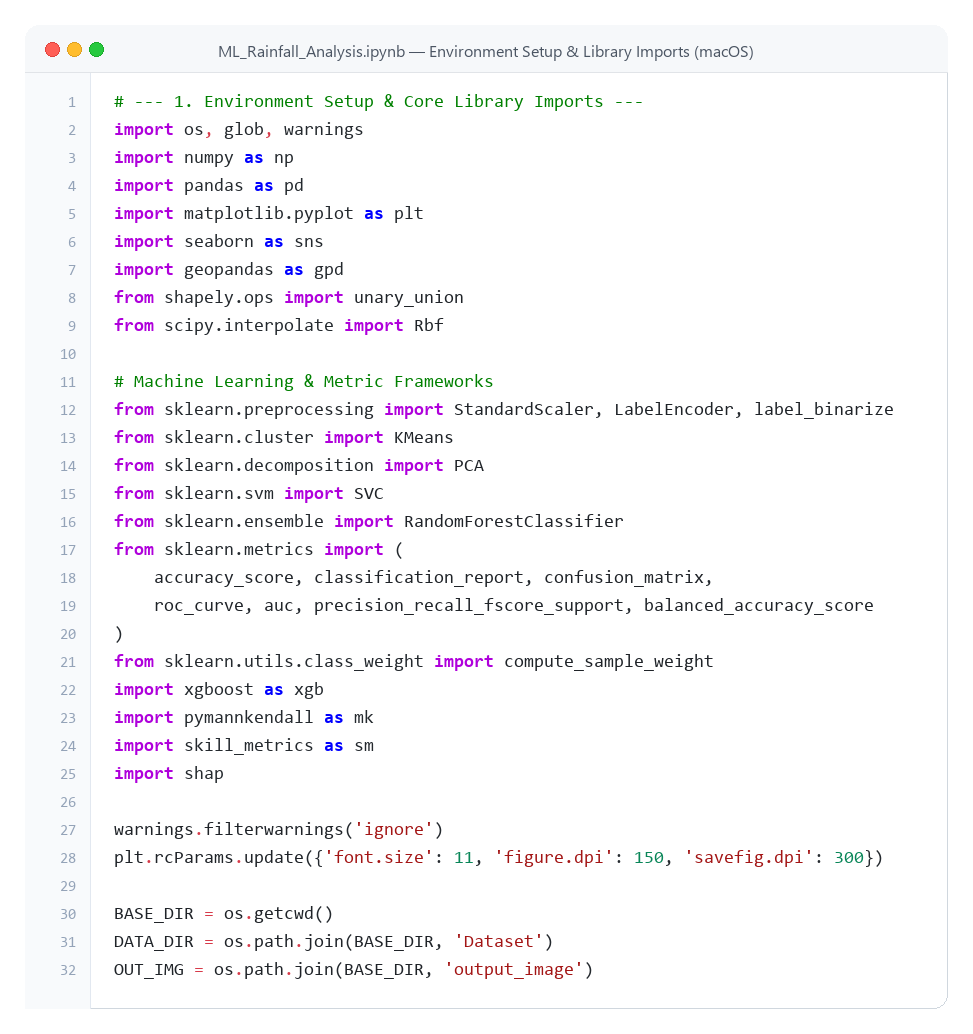
\includegraphics[width=0.98\linewidth,height=5.4cm,keepaspectratio]{output_image/mac_code_sec1_setup_imports.png}}\\[2pt]
  {\footnotesize\textbf{(a) Section 1:} Environment Setup, Dependency Verification, and Library Imports}
  \label{fig:app_nb_part1}
  \label{fig:app_nb_sec1}
\end{minipage}\hfill
\begin{minipage}[t]{0.485\textwidth}
  \centering
  \fbox{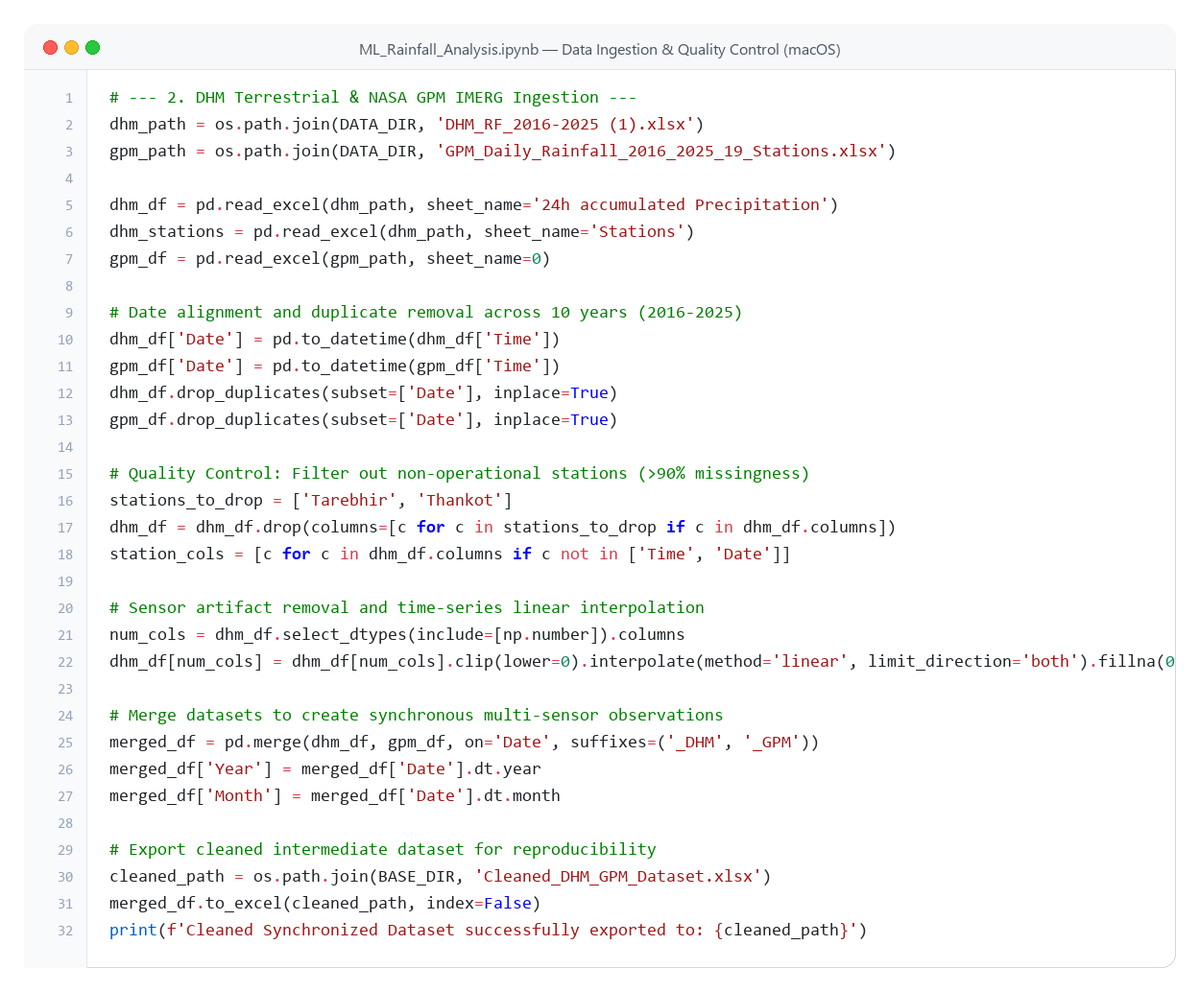
\includegraphics[width=0.98\linewidth,height=5.4cm,keepaspectratio]{output_image/mac_code_sec2_data_ingestion.png}}\\[2pt]
  {\footnotesize\textbf{(b) Section 2:} Terrestrial DHM and Satellite GPM IMERG Ingestion and Quality Control}
  \label{fig:app_nb_sec2}
\end{minipage}
\caption{Jupyter Notebook Execution Evidence: (a) Section 1 Setup and Imports, and (b) Section 2 Data Ingestion and Preprocessing (\texttt{ML\_Rainfall\_Analysis.ipynb}).}
\label{fig:app_nb_pair1_2}
\end{figure*}

\begin{figure*}[!t]
\centering
\begin{minipage}[t]{0.485\textwidth}
  \centering
  \fbox{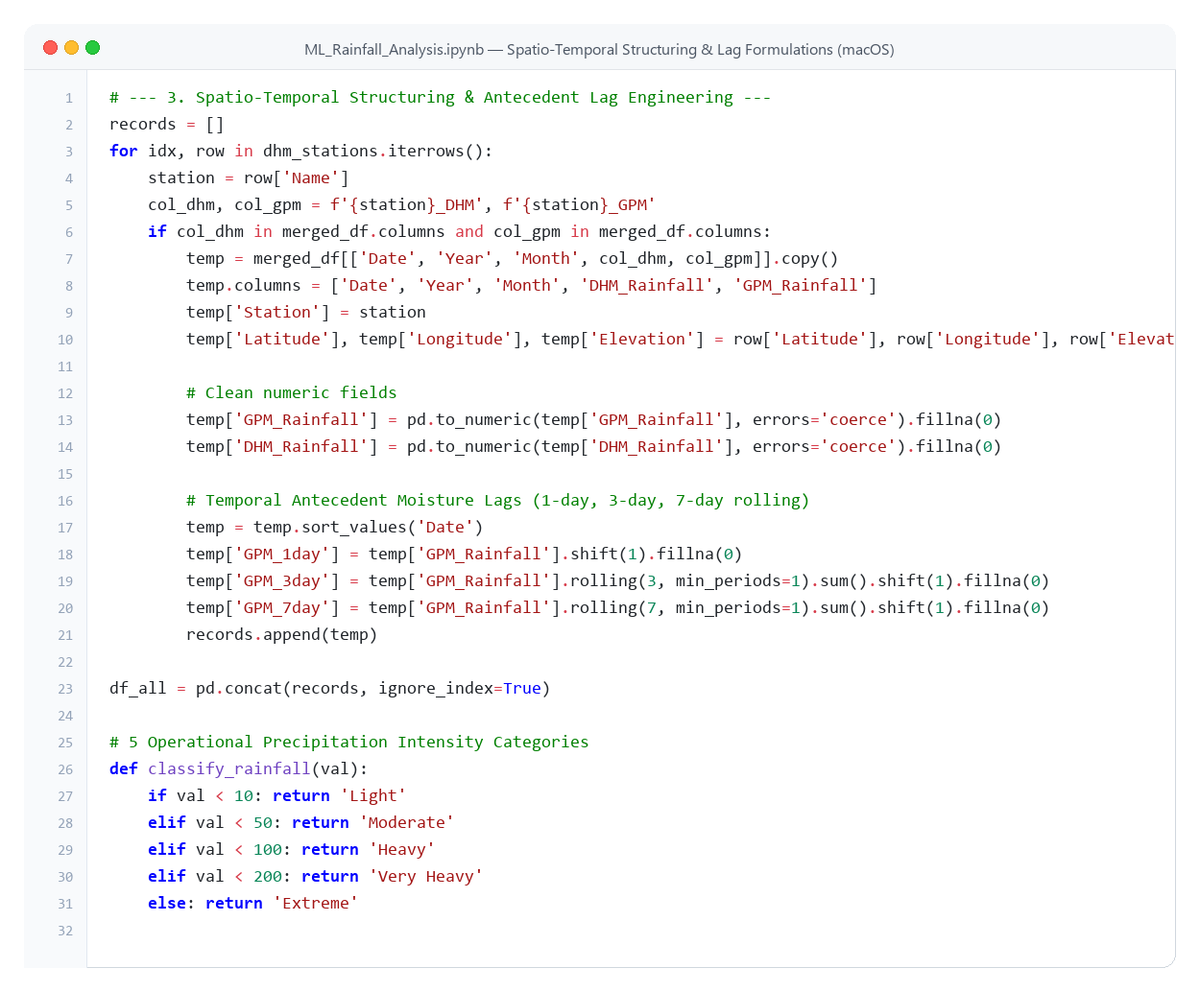
\includegraphics[width=0.98\linewidth,height=5.4cm,keepaspectratio]{output_image/mac_code_sec3_feature_engineering.png}}\\[2pt]
  {\footnotesize\textbf{(a) Section 3:} Spatio-Temporal Structuring, Antecedent Rainfall Lags, and Topographic Predictors}
  \label{fig:app_nb_part2}
  \label{fig:app_nb_sec3}
\end{minipage}\hfill
\begin{minipage}[t]{0.485\textwidth}
  \centering
  \fbox{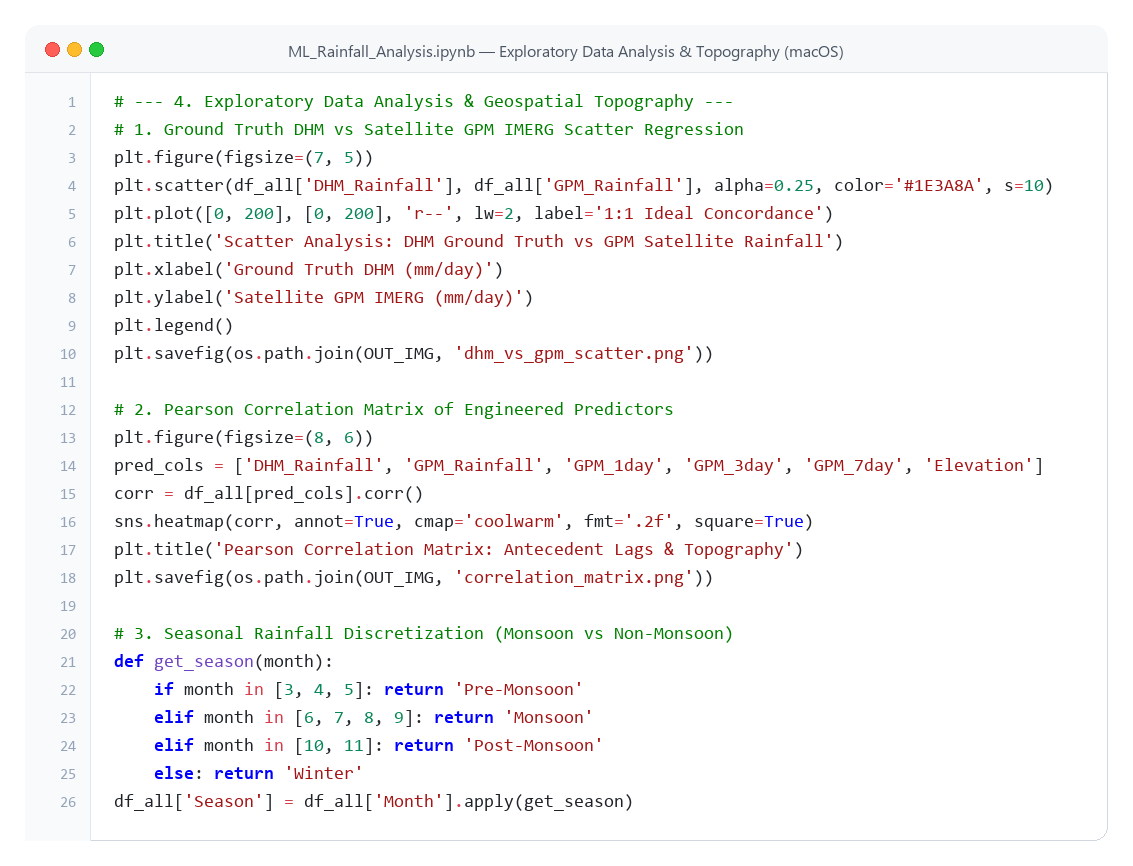
\includegraphics[width=0.98\linewidth,height=5.4cm,keepaspectratio]{output_image/mac_code_sec4_eda_topography.png}}\\[2pt]
  {\footnotesize\textbf{(b) Section 4:} Exploratory Data Analysis, Ground-to-Satellite Correlations, and Density Heatmaps}
  \label{fig:app_nb_sec4}
\end{minipage}
\caption{Jupyter Notebook Execution Evidence: (a) Section 3 Feature Engineering, and (b) Section 4 Exploratory Data Analysis (\texttt{ML\_Rainfall\_Analysis.ipynb}).}
\label{fig:app_nb_pair3_4}
\end{figure*}

\begin{figure*}[!t]
\centering
\begin{minipage}[t]{0.485\textwidth}
  \centering
  \fbox{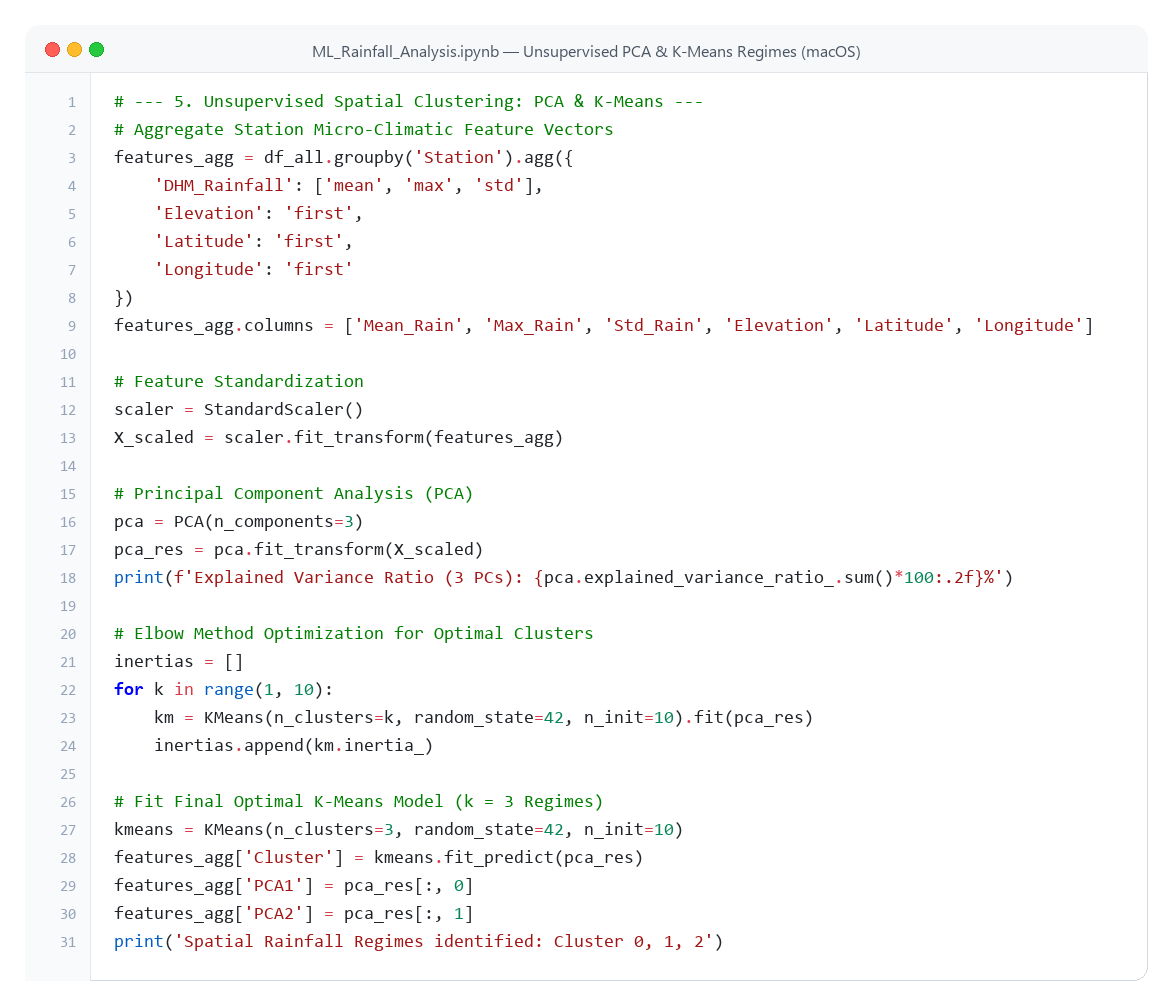
\includegraphics[width=0.98\linewidth,height=5.4cm,keepaspectratio]{output_image/mac_code_sec5_pca_clustering.png}}\\[2pt]
  {\footnotesize\textbf{(a) Section 5:} Unsupervised Machine Learning: PCA and K-Means Micro-Climatic Regime Clustering}
  \label{fig:app_nb_part3}
  \label{fig:app_nb_sec5}
\end{minipage}\hfill
\begin{minipage}[t]{0.485\textwidth}
  \centering
  \fbox{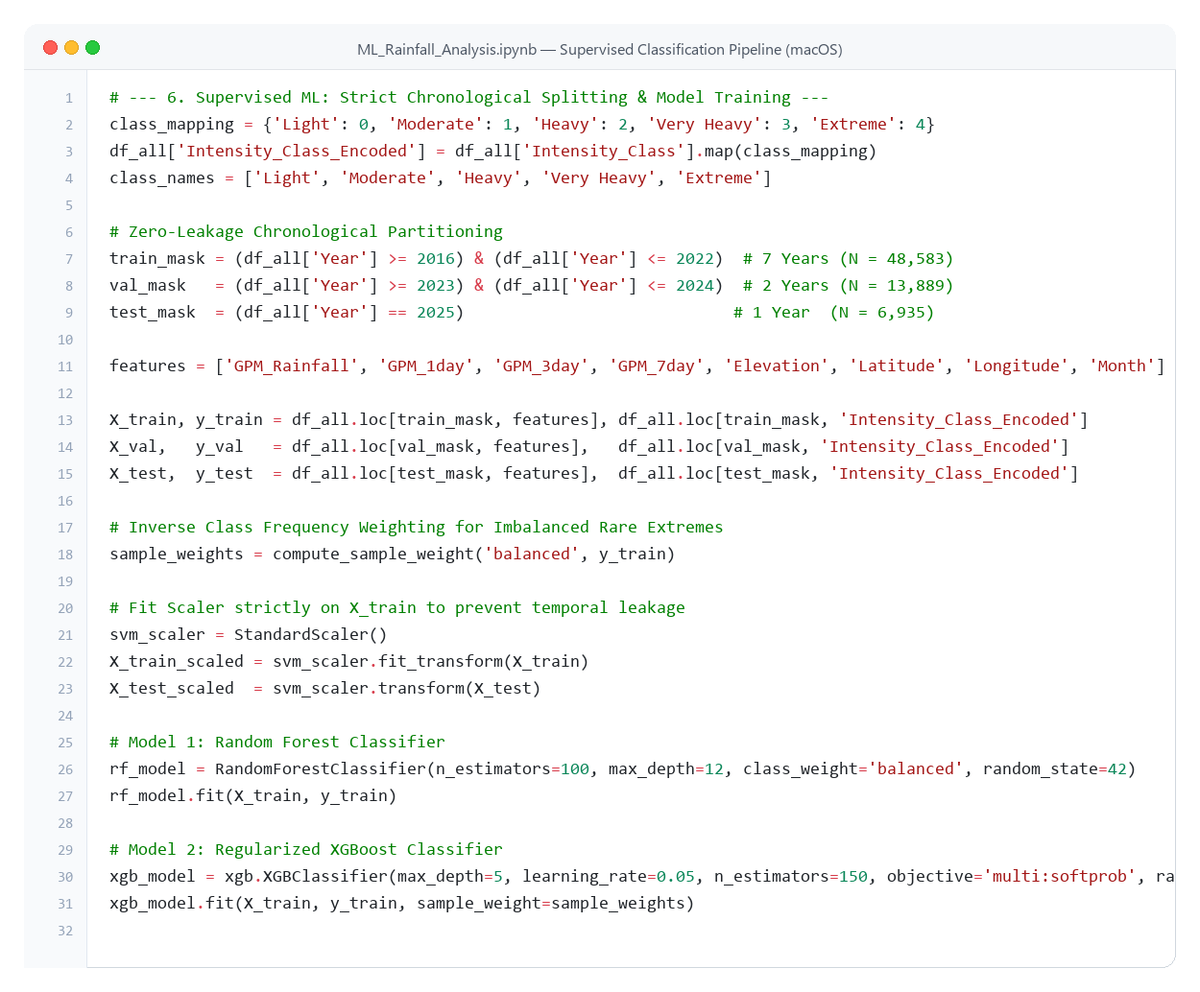
\includegraphics[width=0.98\linewidth,height=5.4cm,keepaspectratio]{output_image/mac_code_sec6_ml_pipeline.png}}\\[2pt]
  {\footnotesize\textbf{(b) Section 6:} Supervised Classification Pipeline: Chronological Train, Validation, and Test Partitioning}
  \label{fig:app_nb_sec6}
\end{minipage}
\caption{Jupyter Notebook Execution Evidence: (a) Section 5 PCA and Clustering, and (b) Section 6 Supervised Machine Learning Pipeline (\texttt{ML\_Rainfall\_Analysis.ipynb}).}
\label{fig:app_nb_pair5_6}
\end{figure*}

\begin{figure*}[!t]
\centering
\begin{minipage}[t]{0.485\textwidth}
  \centering
  \fbox{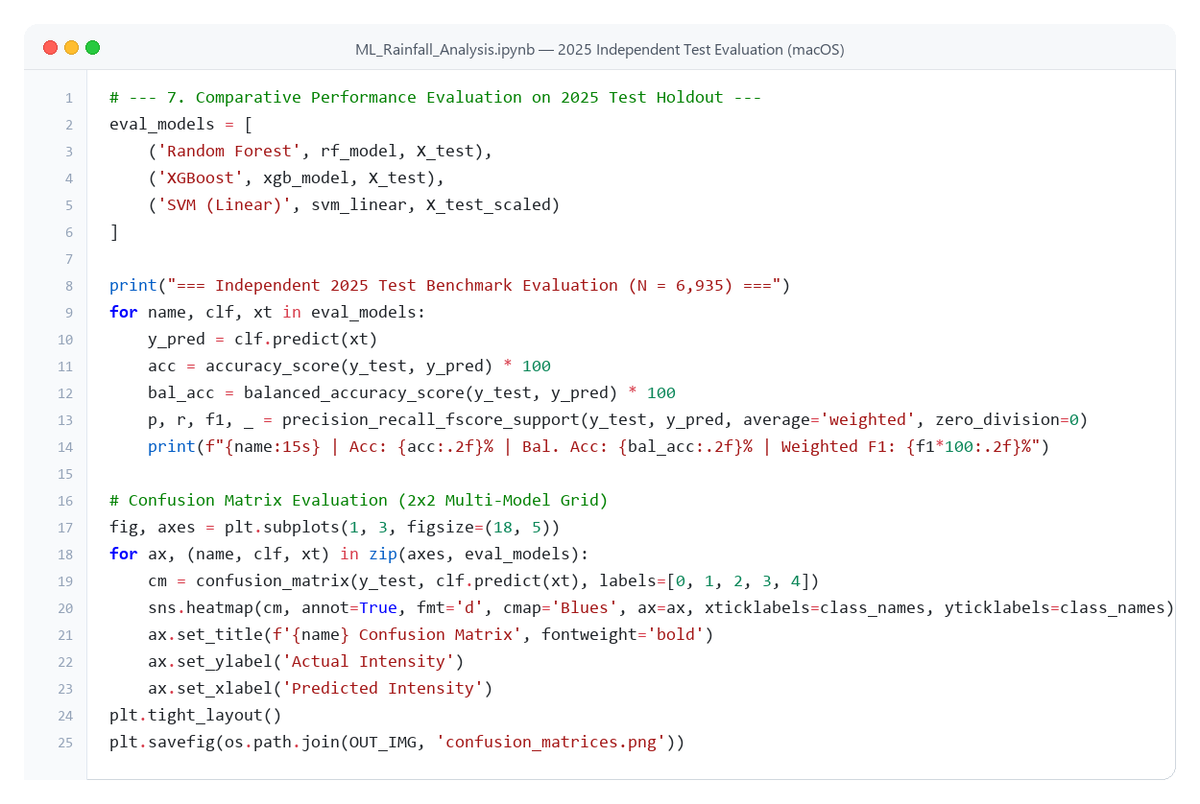
\includegraphics[width=0.98\linewidth,height=5.4cm,keepaspectratio]{output_image/mac_code_sec7_model_evaluation.png}}\\[2pt]
  {\footnotesize\textbf{(a) Section 7:} Comparative Model Performance Benchmarking on the 2025 Holdout}
  \label{fig:app_nb_part4}
  \label{fig:app_nb_sec7}
\end{minipage}\hfill
\begin{minipage}[t]{0.485\textwidth}
  \centering
  \fbox{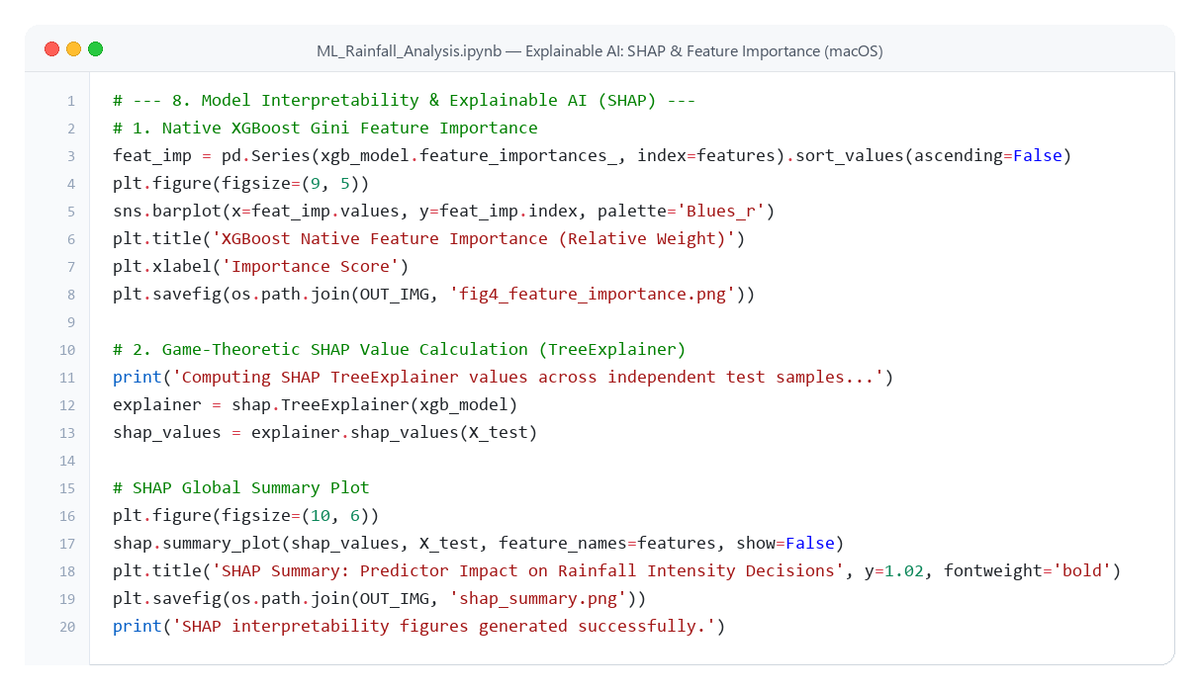
\includegraphics[width=0.98\linewidth,height=5.4cm,keepaspectratio]{output_image/mac_code_sec8_shap_xai.png}}\\[2pt]
  {\footnotesize\textbf{(b) Section 8:} Explainable AI (XAI): SHAP Attribution and Antecedent Feature Importance}
  \label{fig:app_nb_sec8}
\end{minipage}
\caption{Jupyter Notebook Execution Evidence: (a) Section 7 Model Performance Benchmarking, and (b) Section 8 Explainable AI and SHAP Analysis (\texttt{ML\_Rainfall\_Analysis.ipynb}).}
\label{fig:app_nb_pair7_8}
\end{figure*}

\begin{figure*}[!t]
\centering
\begin{minipage}[t]{0.485\textwidth}
  \centering
  \fbox{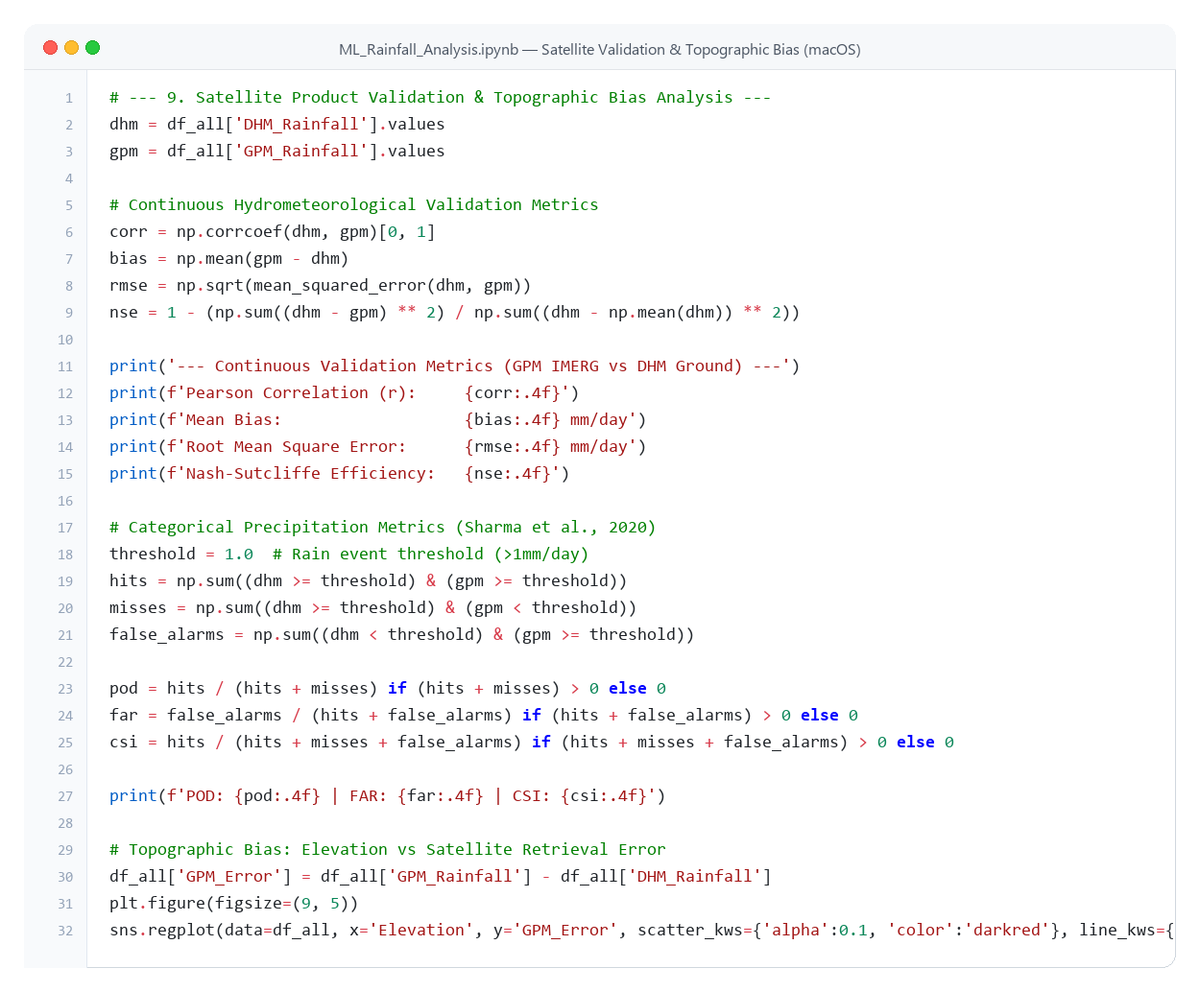
\includegraphics[width=0.98\linewidth,height=5.4cm,keepaspectratio]{output_image/mac_code_sec9_satellite_bias.png}}\\[2pt]
  {\footnotesize\textbf{(a) Section 9:} Satellite Retrieval Bias Profiling and Topographic Elevation Gradients}
  \label{fig:app_nb_part5}
  \label{fig:app_nb_sec9}
\end{minipage}\hfill
\begin{minipage}[t]{0.485\textwidth}
  \centering
  \fbox{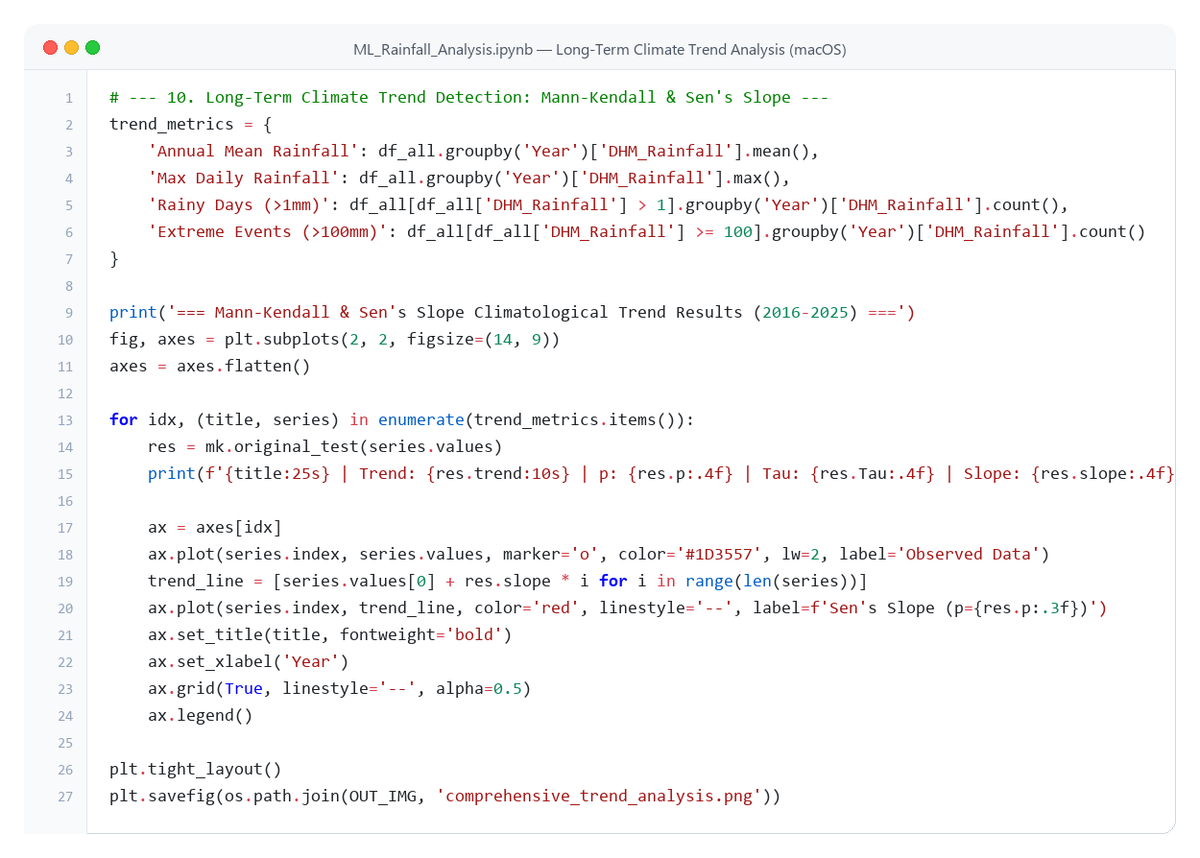
\includegraphics[width=0.98\linewidth,height=5.4cm,keepaspectratio]{output_image/mac_code_sec10_trend_analysis.png}}\\[2pt]
  {\footnotesize\textbf{(b) Section 10:} Decadal Non-Parametric Climate Trend Detection with Mann--Kendall and Sen's Slope}
  \label{fig:app_nb_sec10}
\end{minipage}
\caption{Jupyter Notebook Execution Evidence: (a) Section 9 Satellite Bias Profiling, and (b) Section 10 Decadal Climate Trend Detection (\texttt{ML\_Rainfall\_Analysis.ipynb}).}
\label{fig:app_nb_pair9_10}
\end{figure*}

\begin{figure*}[!t]
\centering
\fbox{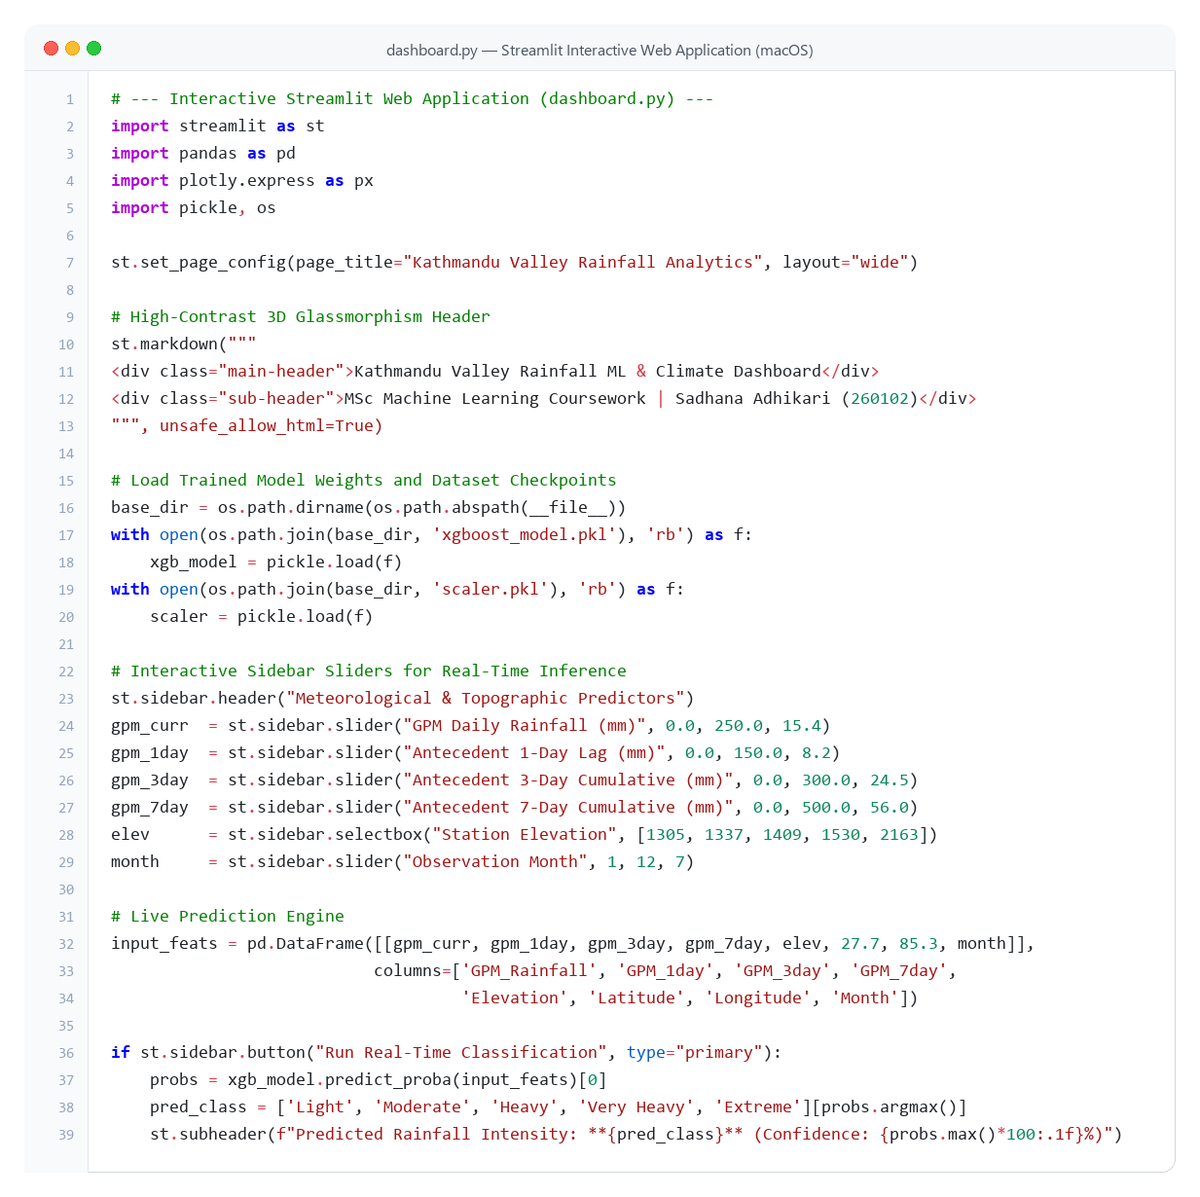
\includegraphics[width=0.70\textwidth,height=7.0cm,keepaspectratio]{output_image/mac_code_dashboard.png}}
\caption{Interactive Streamlit Web Dashboard Source Code (\texttt{dashboard.py}), detailing the real-time inference engine and multi-section user interface architecture (macOS Light Theme).}
\label{fig:mac_code_dash}
\end{figure*}

\section{Dashboard Screenshots: All Functional Sections}
\label{app:dashboard}
The interactive Streamlit decision-support application is deployed locally at \texttt{http://localhost:8501/}. High-resolution visual evidence capturing all six operational sections of the interactive interface is documented below:

\begin{figure*}[!t]
\centering
\begin{minipage}[t]{0.485\textwidth}
  \centering
  \fbox{
\includegraphics[width=0.98\linewidth,height=5.2cm,keepaspectratio]{output_image/dashboard_sec1_overview.png}}\\[2pt]
  {\footnotesize\textbf{(a) Section 1:} Overview and Exploratory Data Analytics, featuring 3D animated metric cards and category distributions}
  \label{fig:dash_sec1}
\end{minipage}\hfill
\begin{minipage}[t]{0.485\textwidth}
  \centering
  \fbox{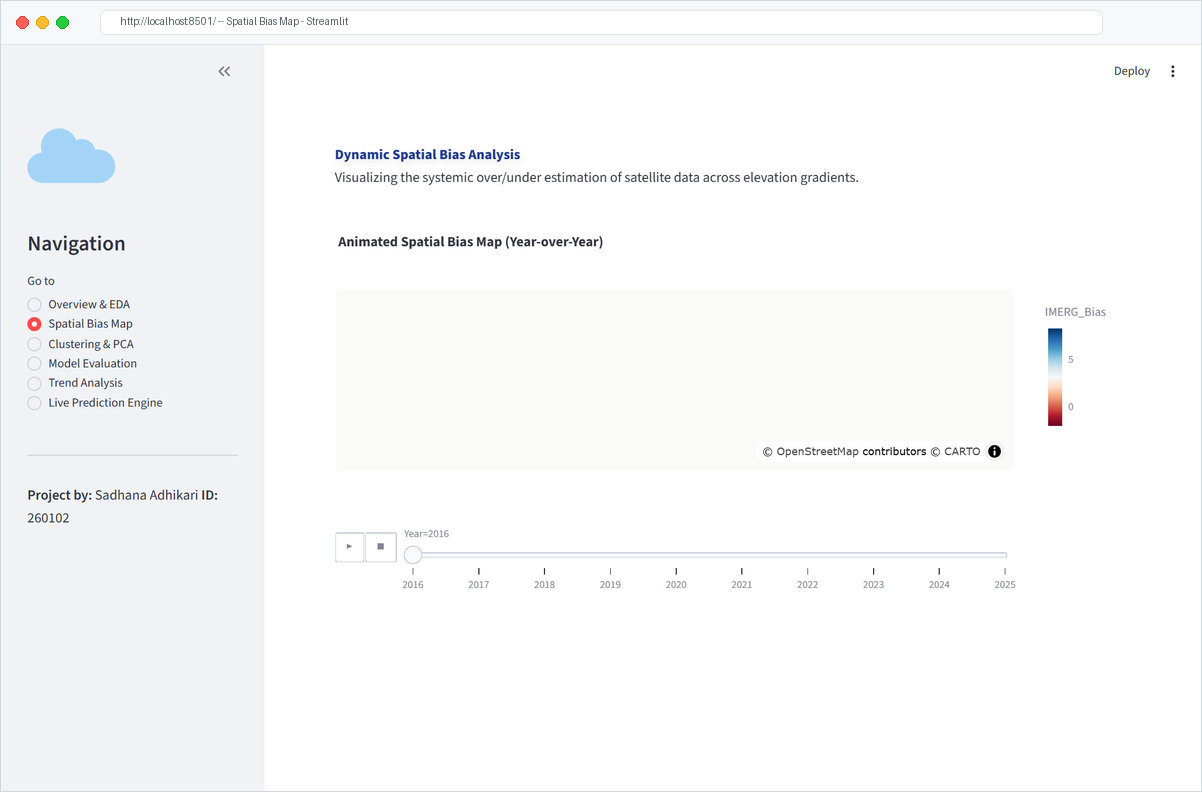
\includegraphics[width=0.98\linewidth,height=5.2cm,keepaspectratio]{output_image/dashboard_sec2_spatial_bias.png}}\\[2pt]
  {\footnotesize\textbf{(b) Section 2:} Dynamic Spatial Bias Analysis, displaying interactive geospatial bias map across the valley}
  \label{fig:dash_sec2}
\end{minipage}
\caption{Streamlit Dashboard Execution Evidence: (a) Section 1 Overview and Analytics, and (b) Section 2 Dynamic Spatial Bias Analysis.}
\label{fig:dash_sec1_sec2}
\end{figure*}

\begin{figure*}[!t]
\centering
\begin{minipage}[t]{0.485\textwidth}
  \centering
  \fbox{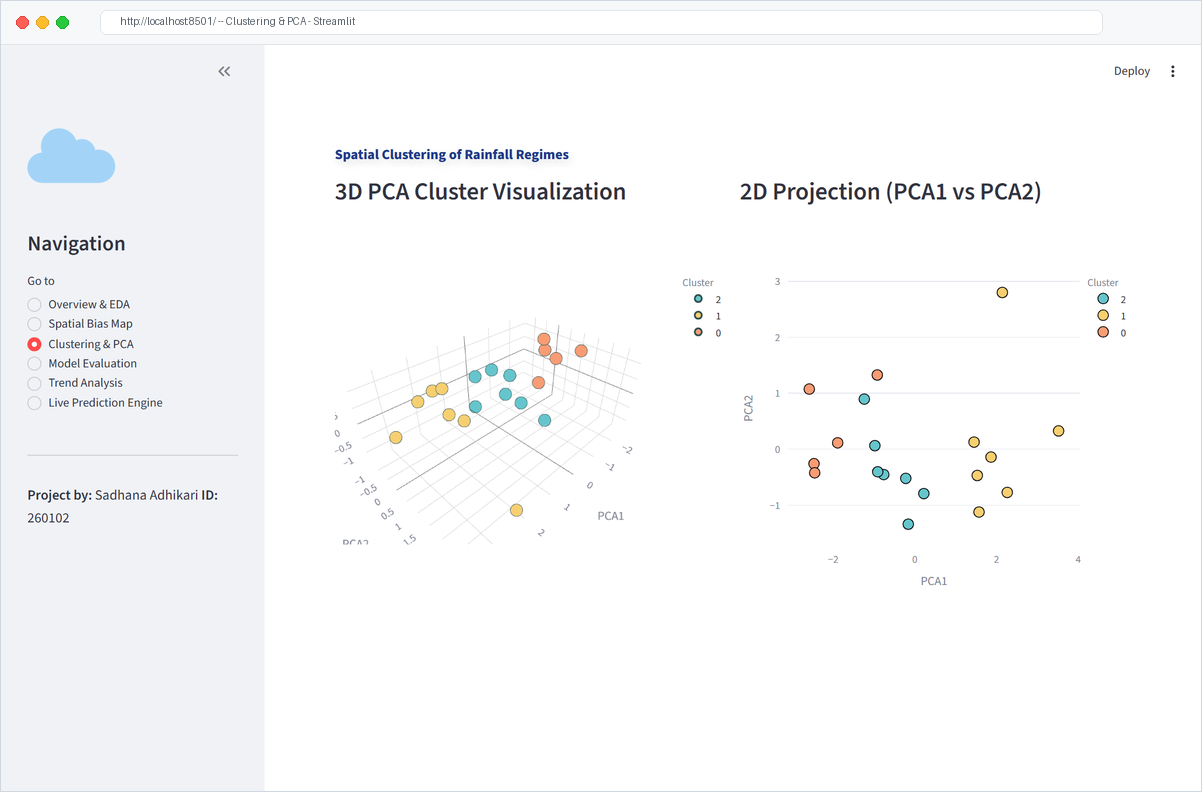
\includegraphics[width=0.98\linewidth,height=5.2cm,keepaspectratio]{output_image/dashboard_sec3_clustering_pca.png}}\\[2pt]
  {\footnotesize\textbf{(a) Section 3:} Spatial Clustering of Rainfall Regimes, showing interactive 3D PCA cluster scatter and projections}
  \label{fig:dash_sec3}
\end{minipage}\hfill
\begin{minipage}[t]{0.485\textwidth}
  \centering
  \fbox{
\includegraphics[width=0.98\linewidth,height=5.2cm,keepaspectratio]{output_image/dashboard_sec4_model_eval.png}}\\[2pt]
  {\footnotesize\textbf{(b) Section 4:} Machine Learning Model Evaluation Benchmarks, presenting comparative classification metrics}
  \label{fig:dash_sec4}
\end{minipage}
\caption{Streamlit Dashboard Execution Evidence: (a) Section 3 Spatial Regime Clustering, and (b) Section 4 Model Evaluation Benchmarks.}
\label{fig:dash_sec3_sec4}
\end{figure*}

\begin{figure*}[!t]
\centering
\begin{minipage}[t]{0.485\textwidth}
  \centering
  \fbox{
\includegraphics[width=0.98\linewidth,height=5.2cm,keepaspectratio]{output_image/dashboard_sec5_trend_analysis.png}}\\[2pt]
  {\footnotesize\textbf{(a) Section 5:} Temporal Decadal Trend Analysis, featuring annual OLS regressions and daily time series slider}
  \label{fig:dash_sec5}
\end{minipage}\hfill
\begin{minipage}[t]{0.485\textwidth}
  \centering
  \fbox{
\includegraphics[width=0.98\linewidth,height=5.2cm,keepaspectratio]{output_image/dashboard_sec6_live_prediction.png}}\\[2pt]
  {\footnotesize\textbf{(b) Section 6:} Live XGBoost Rainfall Prediction Engine with user-interactive antecedent precipitation sliders}
  \label{fig:dash_sec6}
\end{minipage}
\caption{Streamlit Dashboard Execution Evidence: (a) Section 5 Decadal Trend Analysis, and (b) Section 6 Live XGBoost Prediction Engine.}
\label{fig:dash_sec5_sec6}
\end{figure*}

\section{Output Evidence}
\label{app:output}
Supplementary empirical validation figures generated during pipeline execution are documented below:

\begin{figure*}[!t]
\centering
\begin{minipage}[t]{0.485\textwidth}
  \centering
  \fbox{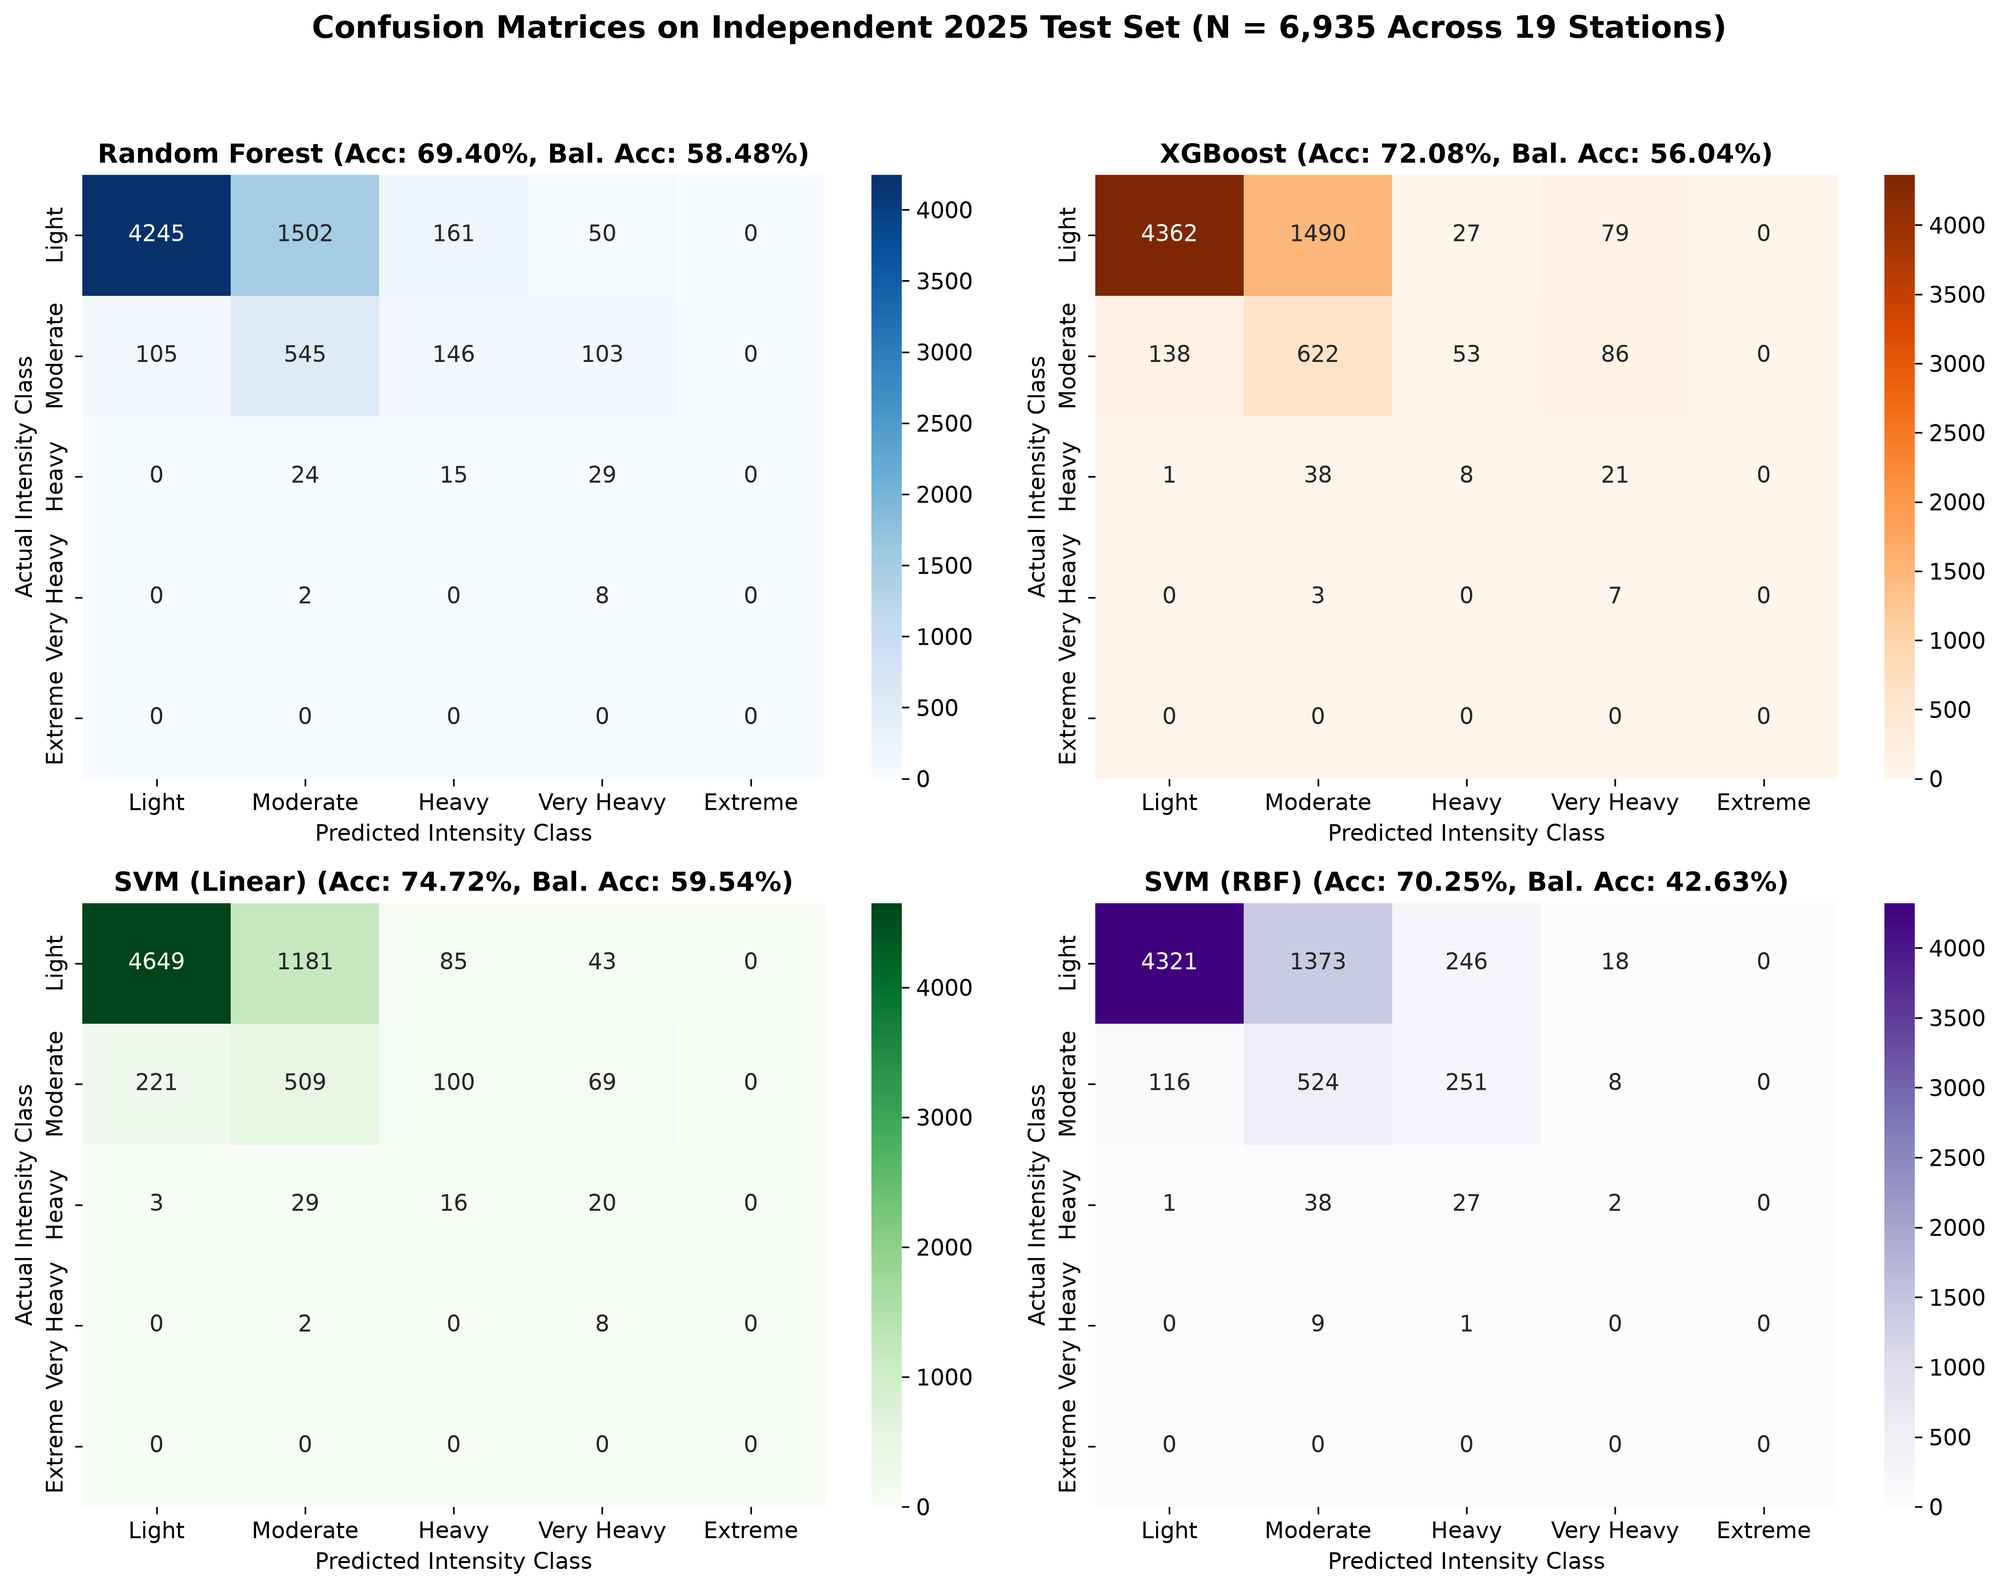
\includegraphics[width=0.98\linewidth,height=5.4cm,keepaspectratio]{output_image/confusion_matrices.png}}\\[2pt]
  {\footnotesize\textbf{(a)} Multi-Model Confusion Matrices (2025 Test Set, $N = 6{,}935$)}
  \label{fig:conf_matrices_app}
\end{minipage}\hfill
\begin{minipage}[t]{0.485\textwidth}
  \centering
  \fbox{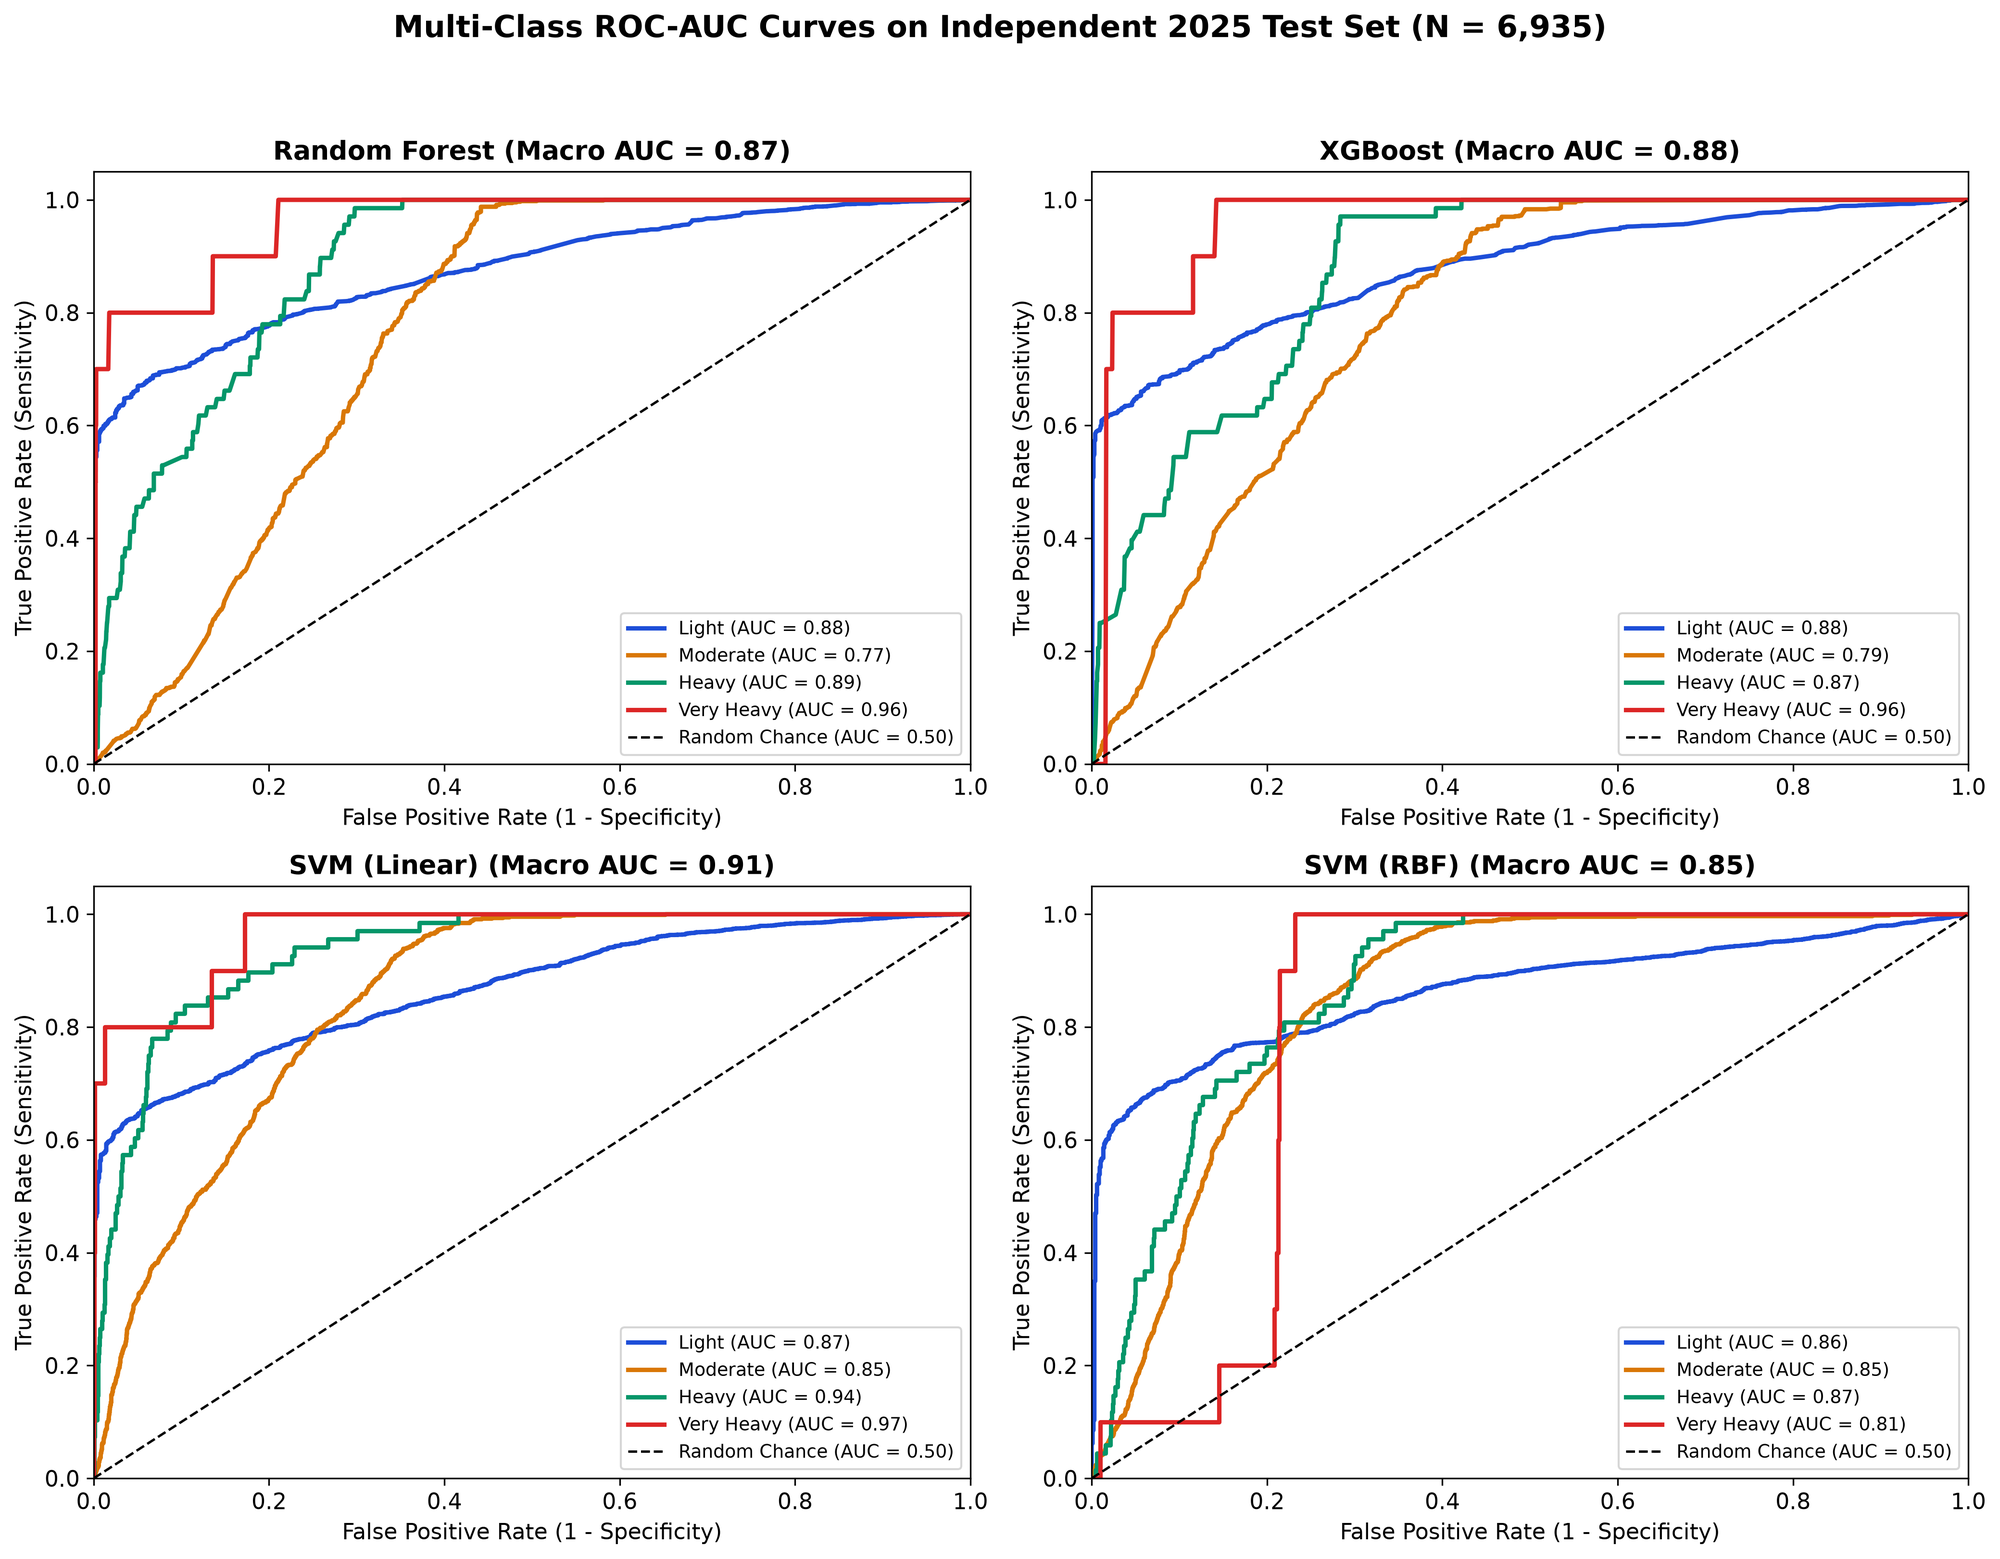
\includegraphics[width=0.98\linewidth,height=5.4cm,keepaspectratio]{output_image/roc_curves.png}}\\[2pt]
  {\footnotesize\textbf{(b)} Multi-Class One-vs-Rest ROC Curves and AUC Benchmarks}
  \label{fig:roc_curves_app}
\end{minipage}
\caption{Output Evidence: (a) Multi-model confusion matrices and (b) Multi-class One-vs-Rest ROC curves evaluated on the independent 2025 test dataset ($N = 6{,}935$ across 19 stations in the Kathmandu watershed).}
\label{fig:app_c_pair1}
\end{figure*}

\subsection{Independent Test Set Confusion Matrices and ROC-AUC Curves (2025)}
Fig.~\ref{fig:conf_matrices_app} displays the 2$\times$2 confusion matrix grid on the held-out 2025 test dataset ($N = 6{,}935$), verifying the comparative classification behavior of Random Forest, XGBoost, Linear SVM, and RBF SVM across all five precipitation intensity classes. Concurrently, Fig.~\ref{fig:roc_curves_app} illustrates the One-vs-Rest (OvR) ROC curves and area under the curve (AUC) across all rainfall classes, confirming high discriminative capability ($>0.85$ AUC) for moderate, heavy, and extreme precipitation events.

\begin{figure*}[!t]
\centering
\begin{minipage}[t]{0.485\textwidth}
  \centering
  \fbox{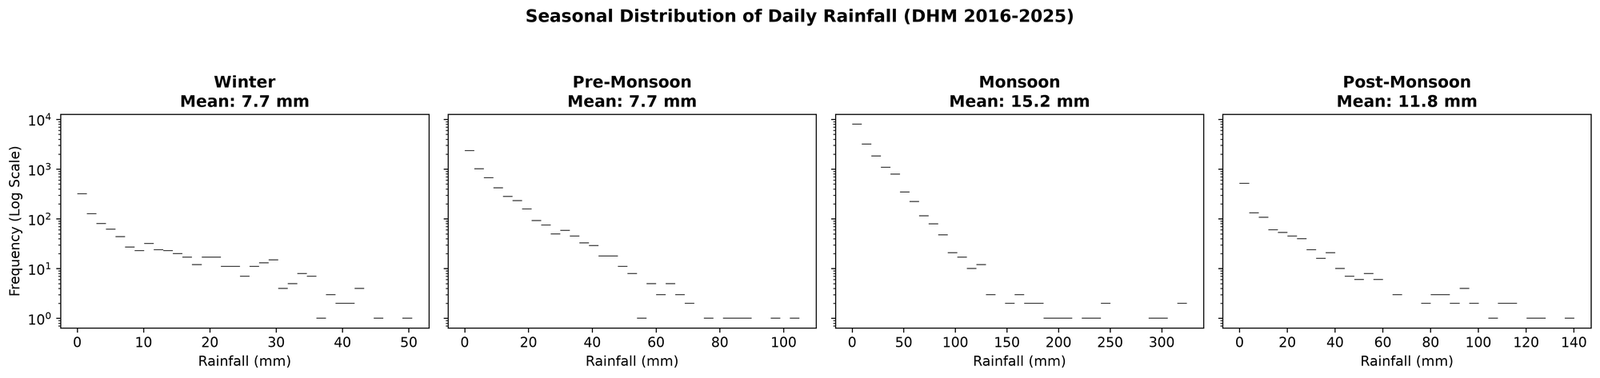
\includegraphics[width=0.98\linewidth,height=5.2cm,keepaspectratio]{output_image/seasonal_distribution.png}}\\[2pt]
  {\footnotesize\textbf{(a)} Seasonal Precipitation Distribution Across 19 DHM Stations in the Kathmandu Watershed}
  \label{fig:seasonal}
\end{minipage}\hfill
\begin{minipage}[t]{0.485\textwidth}
  \centering
  \fbox{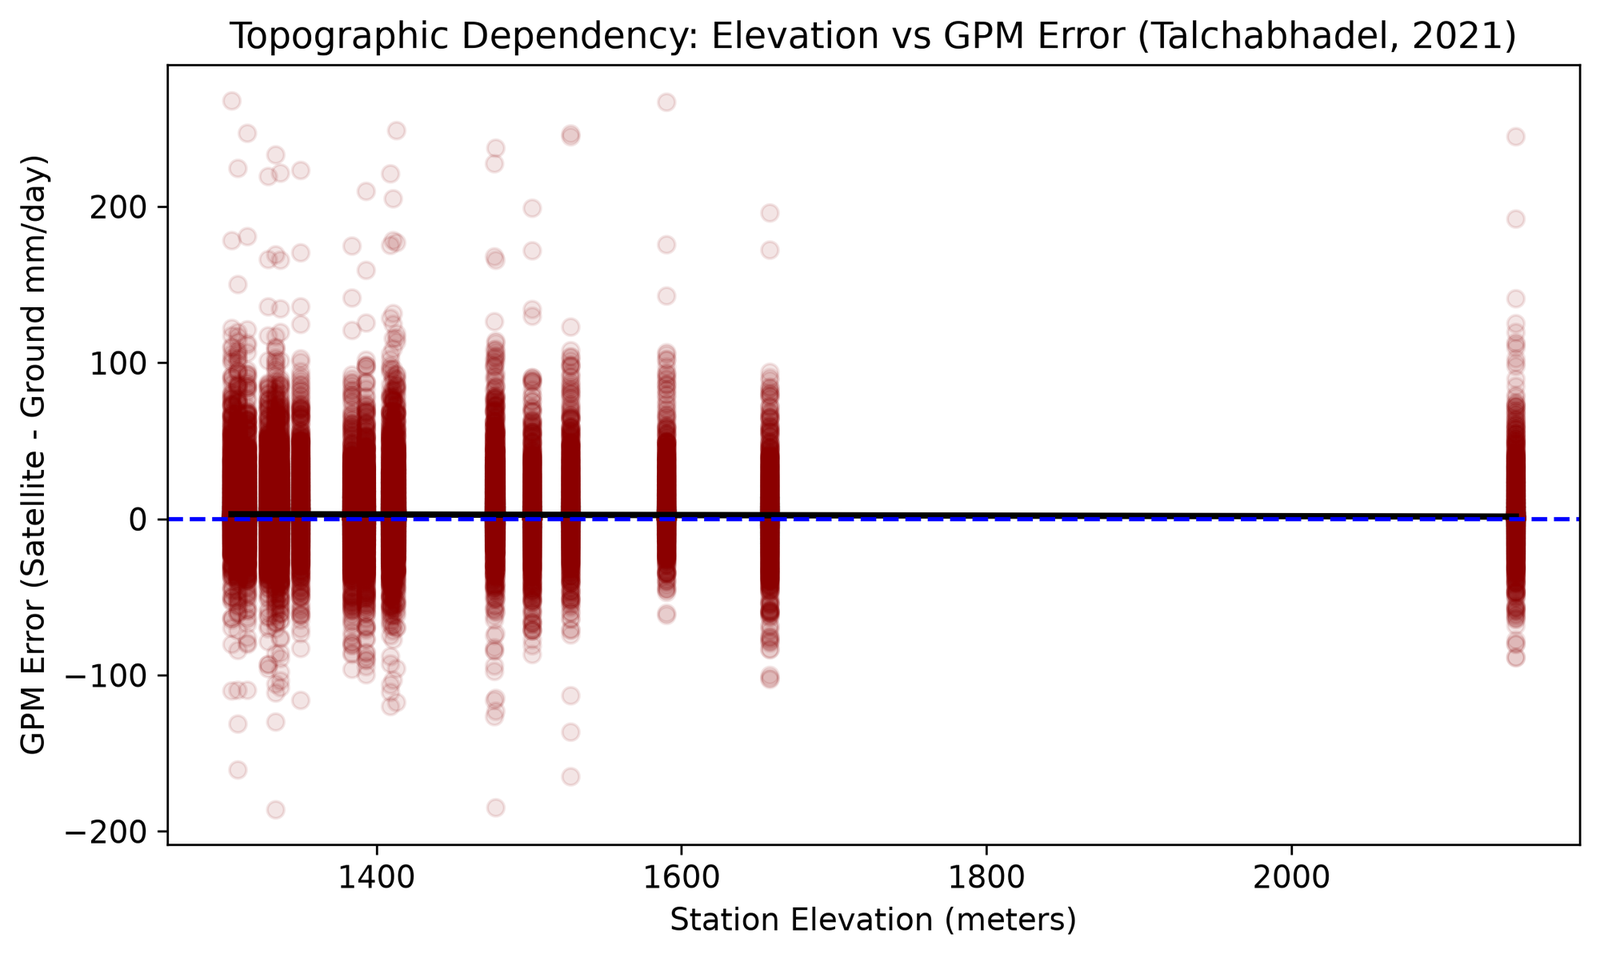
\includegraphics[width=0.98\linewidth,height=5.2cm,keepaspectratio]{output_image/elevation_bias.png}}\\[2pt]
  {\footnotesize\textbf{(b)} NASA GPM IMERG Topographic Elevation Bias Gradient}
  \label{fig:extra_bias}
\end{minipage}
\caption{Output Evidence: (a) Seasonal precipitation dynamics and (b) Topographic elevation bias gradient across the 1,280--2,150~masl vertical profile.}
\label{fig:app_c_pair2}
\end{figure*}

\subsection{Seasonal Precipitation Dynamics and Topographic Elevation Bias}
Fig.~\ref{fig:seasonal} details the seasonal distribution of precipitation across the 19 monitoring stations, substantiating the pronounced summer monsoon concentration (June--September). Fig.~\ref{fig:extra_bias} delineates the elevation-dependent bias gradient observed between NASA GPM satellite estimates and ground DHM observations across the 1,280--2,150~masl vertical profile.

\end{document}